\documentclass[a4paper, 11pt]{article}
\usepackage[utf8]{inputenc}
\usepackage[T1]{fontenc}
\usepackage[french]{babel}
\usepackage{xcolor}
\usepackage[runin]{abstract}
\usepackage[top = 2.5cm, bottom = 2.5cm, left = 1.5cm, right = 1.5cm]{geometry}
\usepackage{float, graphicx, appendix, subcaption, fancyhdr, footmisc, lmodern, amsmath, array}
\usepackage{titlesec}
\usepackage{pdfpages}
\usepackage{lastpage}
\usepackage{newverbs}
\pagestyle{fancy}


% Fonctions =====================
\renewcommand{\headrulewidth}{0pt}
\renewcommand{\footrulewidth}{0pt}
\renewcommand{\arraystretch}{1.5}

\definecolor{mycolor}{RGB}{219, 80, 61}
\titleformat
{\section}
{\color{mycolor}\normalfont\LARGE\sffamily\bfseries}
{\textsf{Projet \thesection}}{1em}{}
\setcounter{tocdepth}{4}
%\setcounter{secnumdepth}{4}


% En-têtes et pieds de pages ================
\cfoot{}
\lfoot{\textcolor{mycolor}{\textsf{L2 SPI \\ 2018-2019}}}
\rfoot{\textcolor{mycolor}{\textsf{Page \thepage / \pageref{LastPage}}}}
 
\rhead{
	\textcolor{mycolor}{\textsf{\rightmark}}
} 

\lhead{
	\textcolor{mycolor}{\textsf{Simulation numérique II -- Mathieu MARÉCHAL}}
}


\begin{document}
	\begin{titlepage}
		\begin{center}
			\huge{Mathieu MARÉCHAL}
				\vskip 3cm
			\Huge Simulation Numérique II
				\vskip 0.25cm
			\Large{Nom de code: Dém***ez-vous !}
				\vskip 3.5cm
					\rule{\linewidth}{0.2mm}\vspace{6mm}\\
			\textbf{\Huge{}}
			\Huge{Compte-rendu des projets}
						\rule{\linewidth}{0.2mm}\vspace{3mm}\\
				\vskip 4.5cm
			\LARGE{Encadrants: C. Desjouy, S. Raetz\\L2 SPI\\ 2018 - 2019\\}
				\vskip 2cm
			\begin{figure}[H]
				\centering
  				
\includegraphics[width=200pt]{logo_univlemans.png}
  				\setcounter{figure}{0}
  				\setcounter{page}{2}
			\end{figure}
		\end{center}
	\end{titlepage}
	
%\newpage
%\addcontentsline{toc}{section}{Introduction}
%\section*{Introduction}


\newpage
\addcontentsline{toc}{section}{Table des matières}
\tableofcontents
\newpage



\section{La balle}

L'objectif de ce projet est de modéliser la trajectoire d'une ou plusieurs balles en prenant en compte les rebonds. La consigne divise le travail en plusieurs étapes qui consistent à, tout d'abord, calculer et animer la trajectoire sans rebonds d'une balle, puis de prendre en compte les rebonds. Enfin, le programme nécessite d'être capable de calculer plusieurs trajectoires à la fois. J'ai donc décidé de procéder comme cela, en rajoutant des étapes: j'ai tout d'abord cherché à calculer une trajectoire simple et sans animation. Ensuite, j'ai créé les codes successifs dans des fichiers séparés, en rajoutant successivement: les animations, les rebonds, et enfin, plusieurs balles.

\subsection{Calculer la trajectoire}
Tout d'abord, les premières constantes dont va dépendre la trajectoire sont crées:
\begin{itemize}
	\item l'angle initial, $\theta_0$ nommé \verb|a_0|
	\item la vitesse initiale $v_0$, notée \verb|v_0|
	\item plus tard, le temps de départ $t_0$ (\verb|t_0|) sera utilisé
\end{itemize}
Ensuite, on implémente les équations déterminant la position du projectile en fonction des constantes précédentes:
\[ \left \{
\begin{array}{c @{= \quad} c}
	d_x & v_0 t \text{cos} (\theta) + d_{0_x}\\
	d_y &- \frac{1}{2} g t^2 + v_0 t \text{sin}(\theta) + d_{0_y}
\end{array}
\right. \]

Il est maintenant possible de calculer la trajectoire mais la première question qui se pose est: quand doit-on arrêter de tracer la trajectoire ? En effet, si on trace la trajectoire sur un temps \verb|t_balle| fixé, on observera la trajectoire avoir une position $d_y$ négative, avec une pente très élevé, ce qui n'a pas du tout la forme d'une parabole. C'est le premier problème que j'ai rencontré. C'est donc quand le projectile touche le sol qu'il faut arrêter de calculer la trajectoire, quand sa position en y vaut 0 $\Leftrightarrow d_y = 0$. Pour cela, il faut calculer le temps de course du projectile, en résolvant l'équation $d_y = 0$. Il est alors possible de désigner une variable \verb|t_max| qui calcule cette solution, ce qui permet de définir la limite du vecteur de temps \verb|t_balle|.
	\begin{verbatim}
	
		t_max = (2 * v_0 * np.sin(a_0)) / g + t_0   
		t_balle = np.arange(t_0, t_max, 0.1)
	\end{verbatim}

Par la suite, on peut animer la trajectoire du projectile. Pour cela, c'est la \verb|FuncAnimation| du module \verb|matplotlib.animation| qui sera utilisée, car elle utilise une fonction pour animer les données calculées et non une boucle \verb|for| comme utilise l'\verb|ArtistAnimation|. Ce choix est justifié aussi par le fait que le programme sera mis sous la forme d'une classe par la suite. 

\begin{figure}[H]
	\centering
	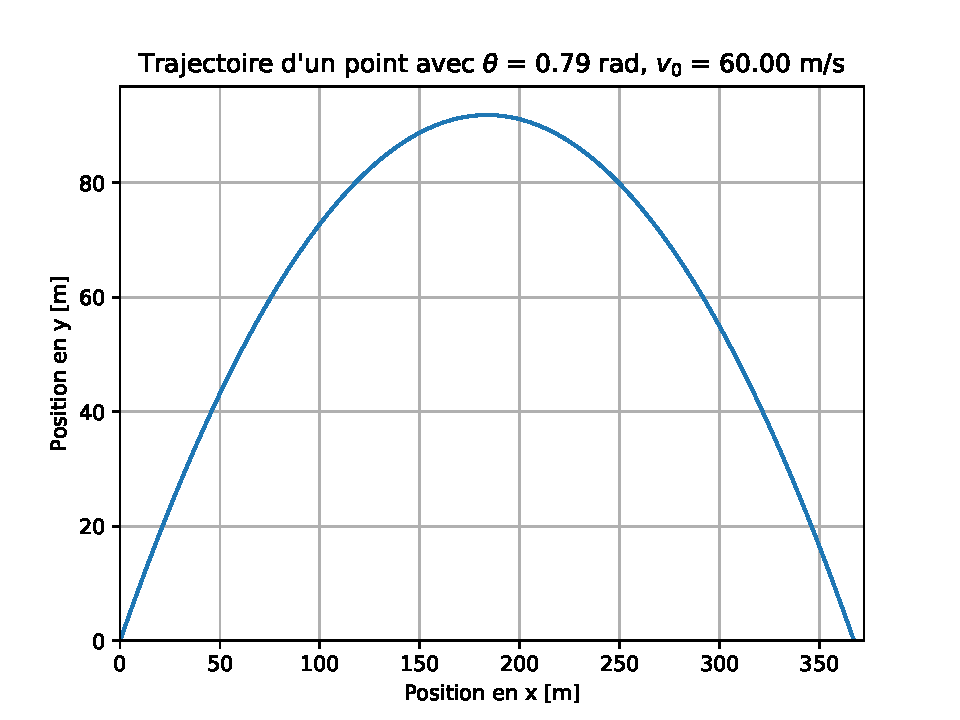
\includegraphics[scale=0.5]{Figures/imgtraject_fixe.pdf}
	\caption{Trajectoire fixe d'une balle}
	\label{fig:traject} 
\end{figure}

\subsection{Ajouter les rebonds}

Implémenter les rebonds, paraît assez simple et c'est le cas! Il suffit de déterminer une nouvelle vitesse initiale à la fin du calcul de la trajectoire et d'en calculer une nouvelle, ce qui est très aisé avec une boucle \verb|for| itérant pour le nombre de rebonds souhaités.

Ainsi, on met sous cette boucle la totalité de la section du code réservé au calcul de la trajectoire développé précédemment. A la fin de la boucle, la vitesse initiale est multipliée par un coefficient de restitution $r$, \verb|v_0 = r*v_0| caractérisant la rigidité du sol, et dans l'ensemble, l'élasticité du rebond, c'est-à-dire la quantité d'énergie de la balle absorbée par le sol. La vitesse de la balle va donc diminuer au fur et à mesure des rebonds successifs. L'autre donnée à conserver lors du calcul du rebond est la position horizontal de la trajectoire précédente. On stocke donc la dernière position en x telle que: \verb|d_0_x = d_x| et on ajoute \verb|d_0_x| en offset au calcul de la position. 


\subsubsection{Exemple de bug rencontré: rebonds de la balle}

Néanmoins, dans cette partie du développement de ce programme, des difficultés ont été rencontrées. D'après la figure 2, on voit que la forme de la trajectoire correspond vaguement à la figure recherchée, mais l'amplitude de la trajectoire sur l'axe $y$ diminue très rapidement et la balle part dans les $y$ négatifs.

\begin{figure}[H]
	\centering
	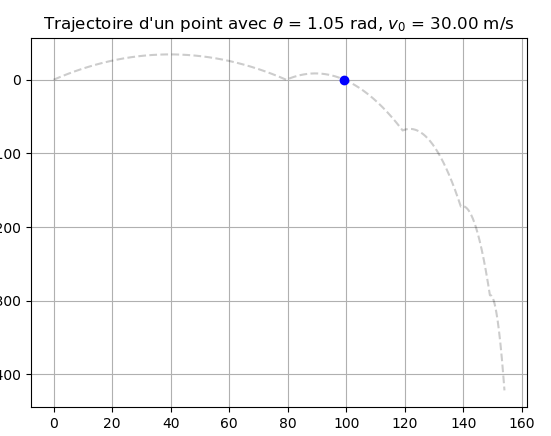
\includegraphics[scale=0.4]{Figures/bug_classe_rebond.png}
	\caption{Exemple de bug au moment de prendre en compte les rebonds pour la balle}
	\label{fig:bug_reb} 
\end{figure}

Cependant, il est possible de remarquer très vite le problème: le temps de la trajectoire \verb|t_max| est le même pour chaque rebond. En effet, cette variable était déterminé au début du programme et faisait partie des conditions initiales. Cependant, comme vu précédemment, \verb|t_max| dépend de l'angle initiale, mais surtout de la vitesse initiale. Comme la vitesse varie après chaque rebond, il faut recalculer \verb|t_max| après chaque rebond.

Notre balle a donc obtenu la capacité de rebondir n fois, mais elle se sent toujours très seule. Nous allons donc adapter le programme pour pouvoir en afficher plusieurs en simultanée.


\subsection{Plus de balles}

Dans cette partie, l'objectif est de pouvoir modéliser la trajectoire de \textbf{n} balles en simultané en définissant des constantes initiales aléatoires. Pour cela, il d'initialiser toutes ces conditions en leur donnant une valeur aléatoire avec le module \verb|random|.

Afin de simplifier le programme dans son ensemble et l'implémentation de cette fonctionnalité, le code sera mis sous la forme d'une classe. La première version de ce programme est  \verb|class_multiball.py|: ce programme contient une classe "Balle" avec une méthode \verb|setup| qui calcule la trajectoire de toutes les balles et une méthode \verb|draw| qui les anime sur une figure. Cette syntaxe n'est cependant pas très cohérente et n'optimise pas les possibilités d'une classe. De plus, chaque méthode exécute un grand nombre d'action au lieu d'une seule.

Ainsi, une deuxième version a été créée: \verb|class_multiball_2.py|. Ce programme contient une classe qui renvoie seulement une liste contenant les positions décrivant la trajectoire d'une balle. Le tracé est effectué à l'extérieur de la classe et fait bien retourner à la classe un objet qui est une unique balle, une illustration de ce que permet la classe est présentée en figure \ref{fig:multiball}.

Ce second programme m'a permis de bien comprendre le fonctionnement d'une classe: ici, la classe représente le "comportement" d'une balle. Néanmoins, l'animation est identique pour les 2 programmes, le seule changement étant la lisibilité et la logique derrière le calcul.


\begin{figure}[H]
\centering
\begin{verbatim}
class Balle_1():
    def setup(self):
        # calcule les trajectoires de n balles
    def draw(self):
        # trace toutes les balles

b = Balle_1()
b.setup()
b.draw()

#==========

class Balle_2():
    def __init__(self):
        # conditions initiales
    def get_tmax(self):
        # retourne le temps de course de la balle
    def change_speed(self): 
        # fait diminuer la vitesse au moment du rebond
    def get_x(self, t):  
        # retourne la position en x de la balle à t secondes
    def get_y(self, t):  
        # retourne la position en y de la balle à t secondes
    def get_parab(self): 
        # retourne une liste contenant les positions pour une première parabole
    def get_rebonds(self):  
        # retourne la trajectoire complète de la balle
    def get_traject(self):
        # adapte la liste de la méthode get_rebonds pour que toutes les 
        # instances de la classe Balle_2 aient la même longueur

b = Balle_2()
b.get_traject()
# Animation 
\end{verbatim}
\caption{Comparaison des 2 versions du programme animant plusieurs projectiles}
\end{figure}

\begin{figure}[H]
	\centering
	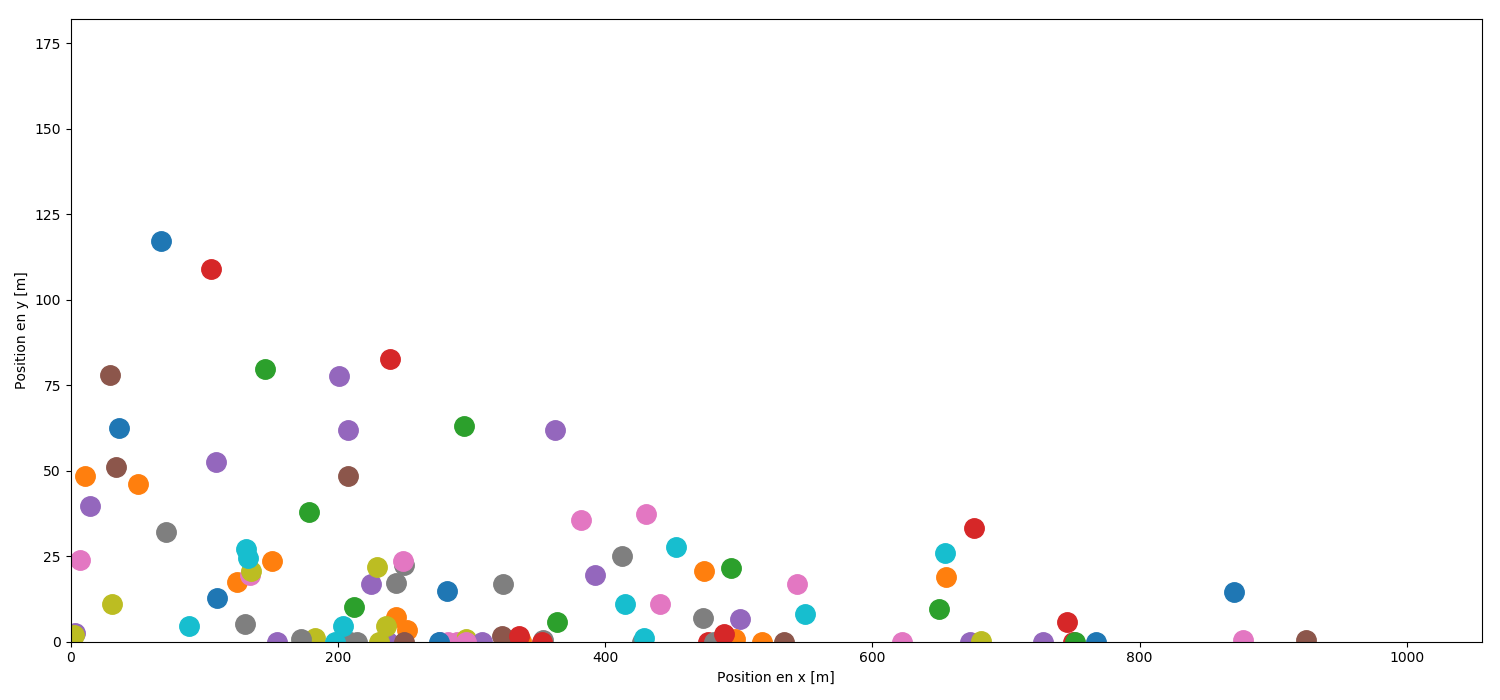
\includegraphics[width=\linewidth]{Figures/multiball.png}
	\caption{Capture d'écran à un instant de la simulation pour 200 balles}
	\label{fig:multiball} 
\end{figure}

Les fichiers présents pour ce projet sont: \verb|class_multiball.py| qui contient la première version de la classe Balle, \verb|class_multiball_2.py| avec la seconde version de la classe Balle et le script \verb|trace_balles.py| avec un exemple d'utilisation de la classe pour animer plusieurs balles.





\newpage
\section{Le tube de Kundt}

Le tube de Kundt est un exemple de système où se propagent des ondes planes en 1D et a été étudié en cours d'Acoustique 1D pendant le semestre 3. L'objet de ce projet est de créer une animation simulant ce tube. 

\begin{figure}[H]
	\centering 
	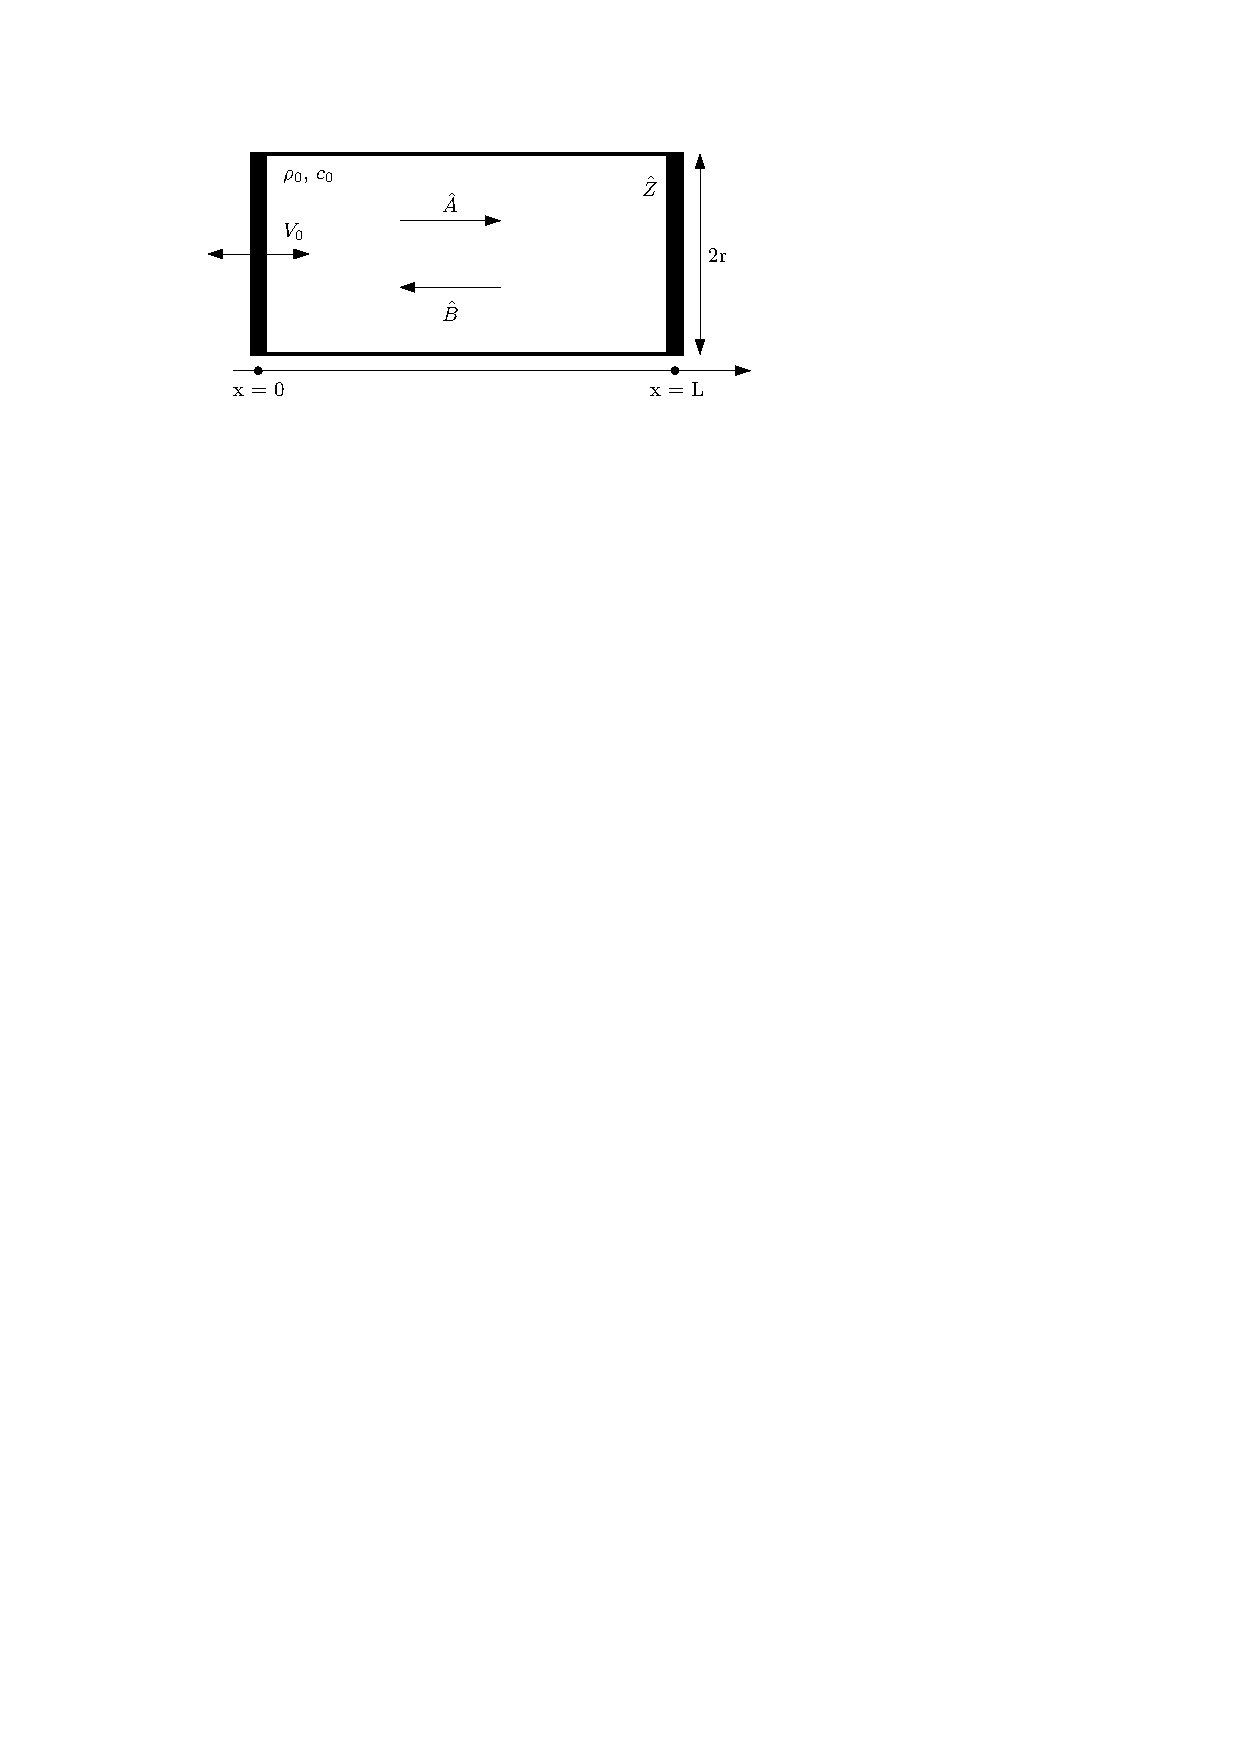
\includegraphics[scale=1]{Figures/tubeKundt_schema.pdf}
	\caption{Schématisation du tube de Kundt}
	\label{fig:schematK} 
\end{figure}

\subsection{Mise en équation du champ acoustique dans le tube}

Le système considéré est donc un tube de Kundt de longueur $L$, cylindrique de diamètre $2r$. Les conditions aux frontières sont: en $x = 0$, un piston oscille à une vitesse $v_0 = V_0 \:  \text{cos}(\omega t)$ et en $x = L$, le tube est fermé par une paroi impédante d'impédance $\hat{Z}$. En considérant un régime monochromatique les amplitudes complexes de pression et de vitesse acoustique en jeu dans ce système sont:

\[ \left \{
\begin{array}{c @{= \quad} c}
	 \hat{p}(x)			& \hat{A} \: e^{-ikx} + \hat{B} \: e^{ikx}\\
	 \hat{v}(x)			& \cfrac{1}{Z_c} \bigg( \hat{A} \: e^{-ikx} - \hat{B} \: e^{ikx} \bigg)
\end{array}
\right. \]
où $\hat{A}$ est l'amplitude de l'onde incidente, $\hat{B}$, l'amplitude de l'onde réfléchie et $k$, le nombre d'onde de l'onde sous réserve que $k = \cfrac{\omega}{c_0}$. $Z_c = \rho_0 \: c_0$ est l'impédance caractéristique du milieu de propagation (ici de l'air donc $\rho$ = 1.2 kg.m$^{-3}$ et $c_0$ = 340 m.s$^{-1}$.  

\subsubsection{Conditions aux frontières}
Les deux conditions limite dans le tube sont:
\begin{itemize}
	\item en x = 0:
\begin{equation*}
	\hat{v} (x=0) = \cfrac{1}{Z_c} \bigg( \hat{A} - \hat{B} \bigg) = V_0
\end{equation*}

	\item en x = L: 
\begin{equation*}
	\hat{Z}(x=L) = \frac{\hat{p} (x=L)}{\hat{v} (x=L)}
\end{equation*}
\end{itemize}

\subsubsection{Champ acoustique de pression et de vitesse dans le tube}
L'application de ces conditions aux frontière permet finalement d'écrire:
\[ \left \{
\begin{array}{c @{= \quad} c}
	 \hat{p}(x)			& \hat{A} \: \bigg( e^{-ikx} + \hat{R}_p \: e^{ikx} \bigg)\\
	 \hat{v}(x)			& \cfrac{\hat{A}}{Z_c} \bigg( e^{-ikx} - \hat{R}_p \: e^{ikx} \bigg)
\end{array}
\right. \]
avec 
\begin{equation*}
	\hat{R}_p = \frac{\eta - 1}{\eta + 1} \: e^{-2ikL} \quad \text{et} \quad \hat{A} = \frac{V_0 Z_c}{1 - \hat{R}_p}
\end{equation*}

\subsection{Modélisation du champ acoustique de pression et de vitesse particulaire sans pertes dans le tube}
En appliquant ces conditions, il est possible de simuler le champ acoustique dans le tube sans pertes. En observant l'animation, la distribution des champs de pression et de vitesses dans le tube de Kundt est visible et observable selon le temps. L'animation est réalisée en stockant l'évolution de chaque champ de pression (incident, réfléchi, total) et chaque champ de vitesse dans des variables séparées afin de pouvoir tracer l'ensemble dans deux sous-figures animées: la première représentant le champ de pression et la deuxième contenant les champs de vitesse. Dans ce cas, le champ acoustique est calculé dans un tube de $L$ = 10 m, $r$ = 2 m, $\eta$ = 0, $\hat{R}_p$ = 0.7 où le champ est monochromatique de fréquence $f$ = 520 Hz, comme le montre la figure \ref{fig:sspertes}.

\begin{figure}[H]
	\centering 
	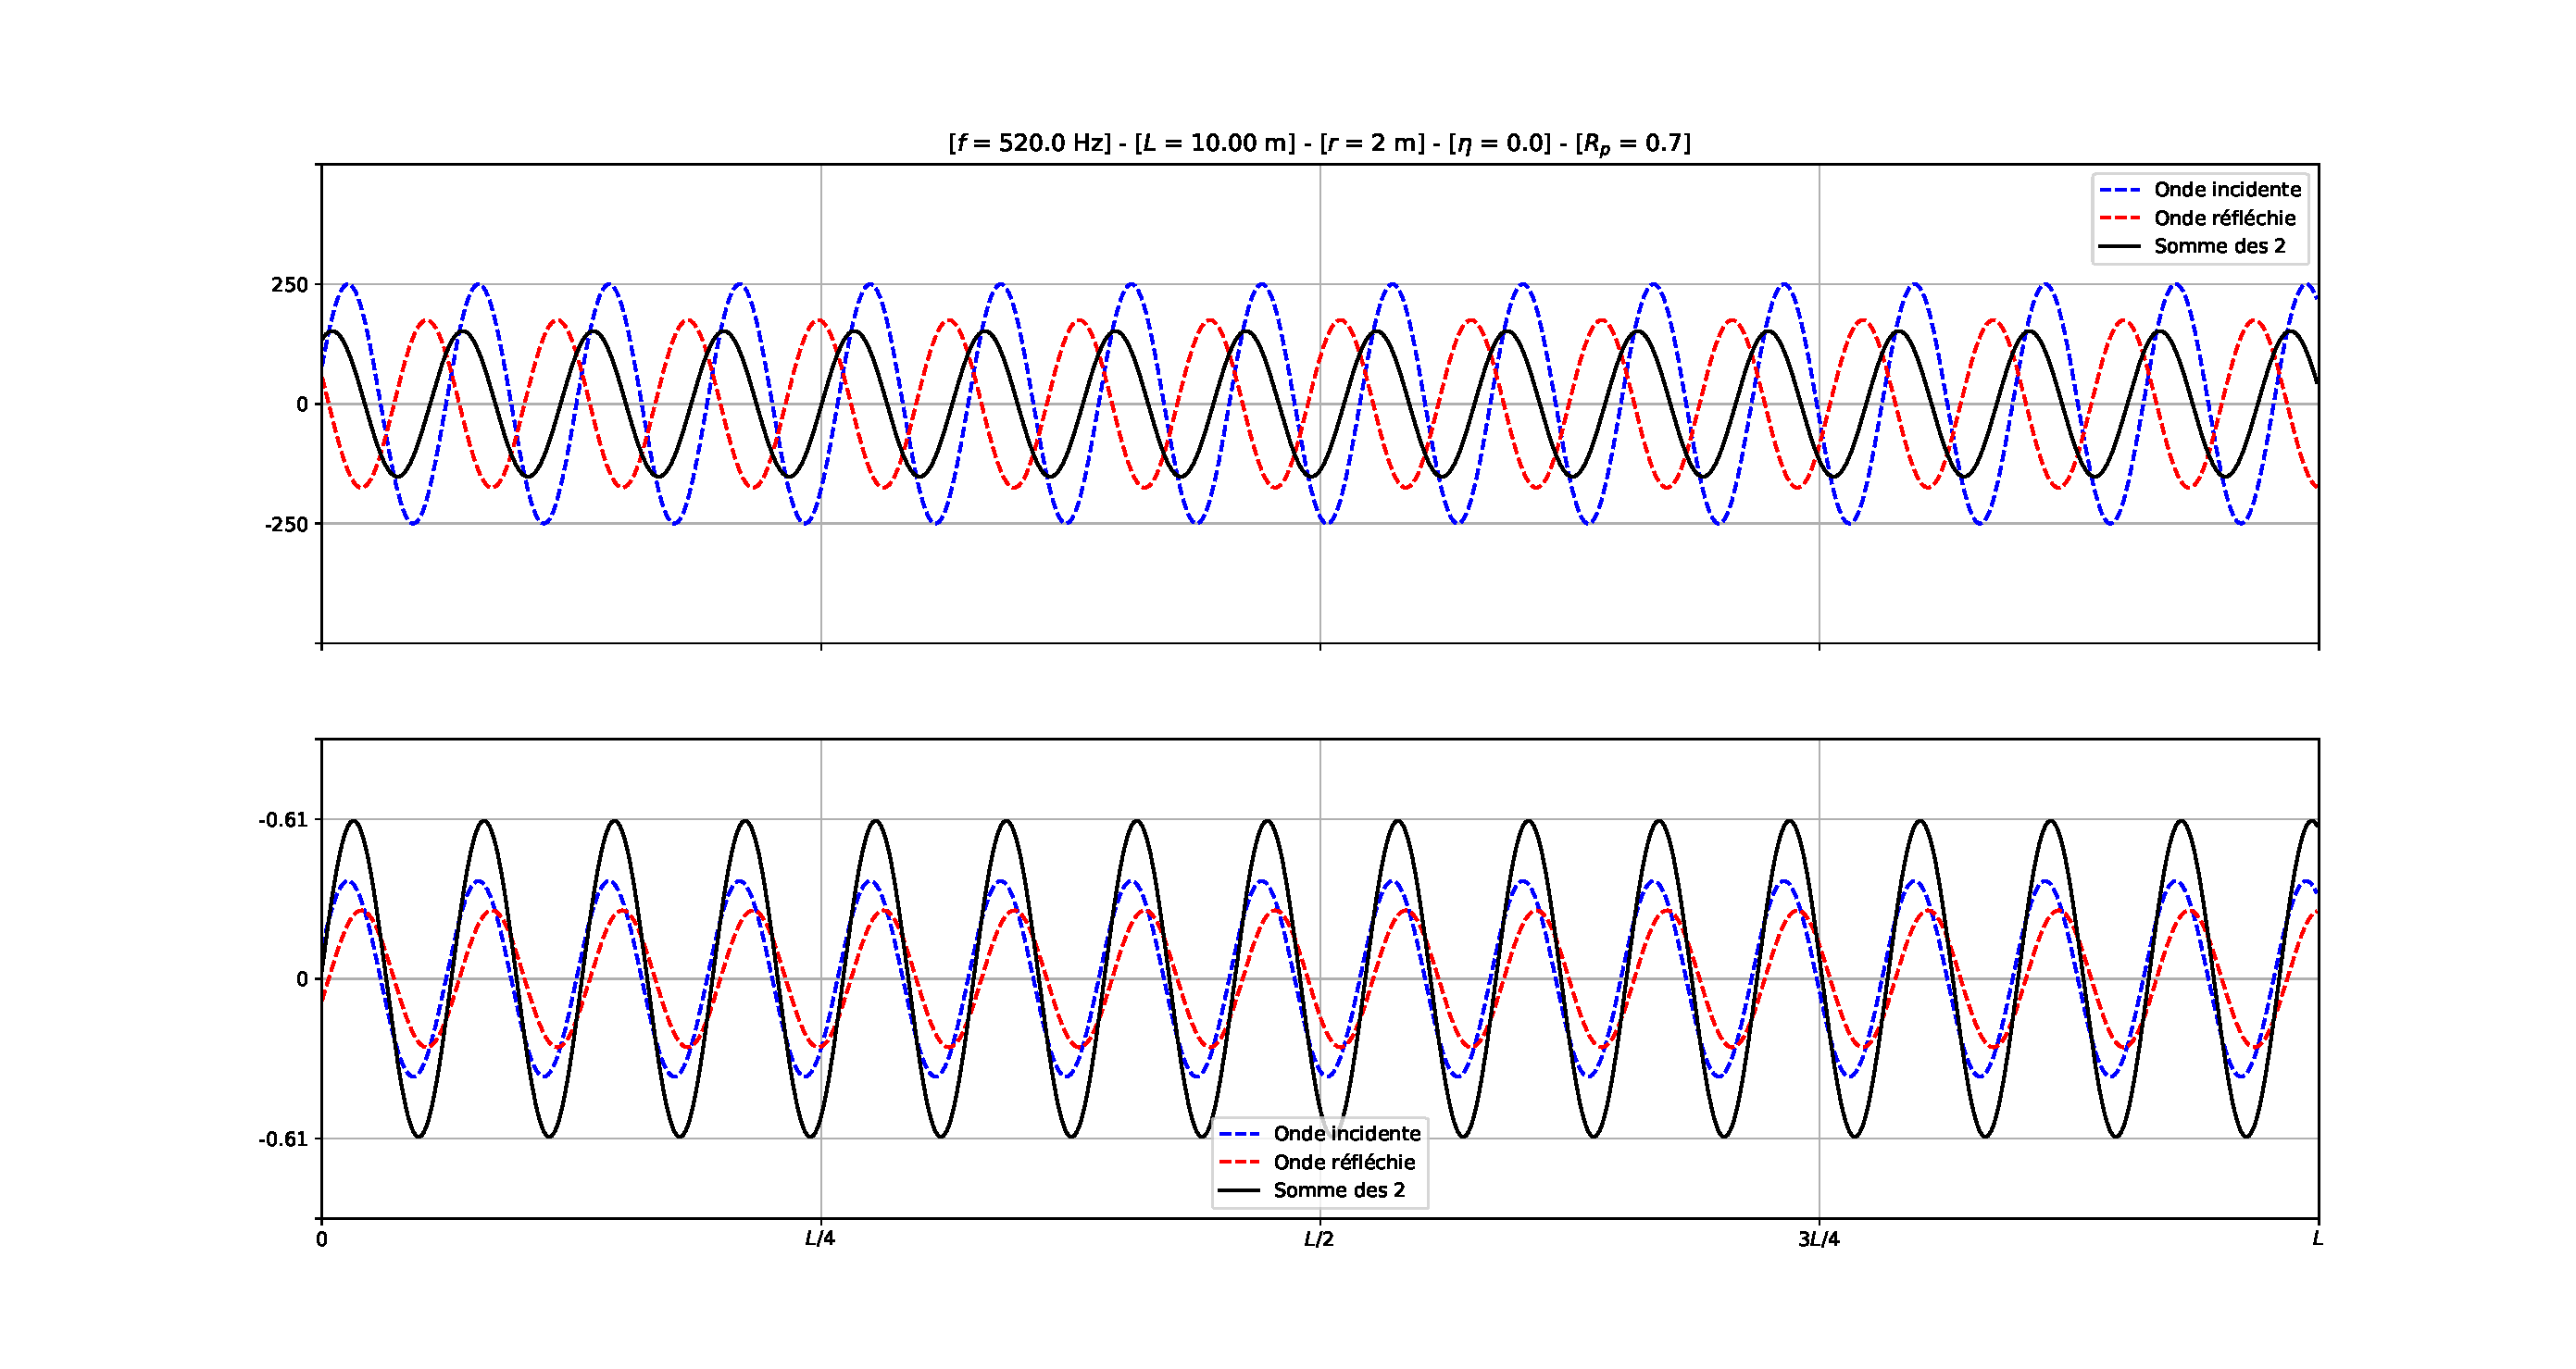
\includegraphics[width=\linewidth]{Figures/tubeKundt_ssperte.pdf}
	\caption{Capture d'écran de la simulation du tube de Kundt sans pertes}
	\label{fig:sspertes} 
\end{figure}

\subsection{Etude du coefficient de réflexion $\hat{R}_p$}
Dans cette partie, le coefficient de réflexion $\hat{R}_p$ est à l'étude. Il a été établi dans l'étude théorique précédemment, l'expression du coefficient de réflexion: il dépend de $\eta$, un coefficient caractérisant l'absorption acoustique du matériau et de la fréquence $f$ de l'onde.
En calculant une matrice contenant les valeurs du coefficient de réflexion en fonction de $\eta$ et de $f$, il est ensuite possible de tracer cette matrice dans un plan ($\eta$, $f$). Comme le coefficient de réflexion est complexe, le module et la phase sont calculés, ainsi que la partie réelle et imaginaire. Les résultats sont présentés en figure \ref{fig:coef_refl}.

\begin{figure}[H]
	\centering 
	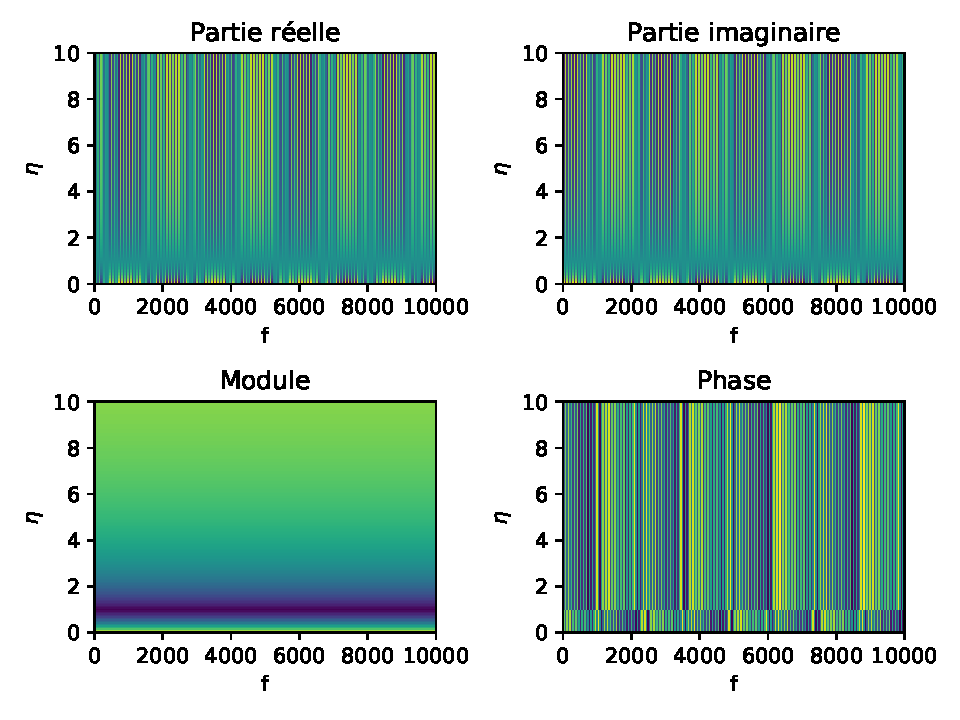
\includegraphics[width=\linewidth]{Figures/coef_refl.pdf}
	\caption{Représentation des modules, phase, parties réelles et imaginaire du coefficient de réflexion dans un plan ($\eta$, $f$)}
	\label{fig:coef_refl}
\end{figure}

La partie réelle et imaginaire représentent une variation sinusoïdale du coefficient de réflexion en fonction de la fréquence: en effet, la fréquence se trouve dans une fonction exponentielle complexe dans l'expression de $\hat{R}_p$, qui, en réelle ou en imaginaire donne une fonction sinusoïdale. Selon $\eta$, il est possible de remarquer une discontinuité pour $\eta = 1$. Autour de cette valeur, le coefficient de réflexion diminue et tend vers 0. Il est cependant uniforme dans les $\eta > 1$. Cette discontinuité se retrouve dans le module et dans la phase: le module vaut 1 autour de $\eta = 0$, 0 pour $\eta = 1$, puis augmente pour les $\eta$ supérieurs. Cette discontinuité montre que, quand le coefficient $\eta$ d'un matériau est autour de 1, celui-ci est parfaitement absorbant car le coefficient de réflexion vaut 0. Le matériau est de plus en plus réfléchissant à mesure que $\eta$ diminue si $\eta < 1$ et augmente si $\eta > 1$.  

\subsection{Simulation du champ acoustique dans le tube avec prise en compte des phénomènes de pertes}

Dans cette dernière partie, la première partie comportant l'étude du champ acoustique est reprise et améliorée afin de prendre en compte les pertes. Les pertes acoustique dans un tube sont de 2 natures: dispersion et dissipation. Le résultat est identique pour les 2 phénomènes: une diminution de l'amplitude à l'extrémité opposée à la source dans le tube. Cependant, ce sont 2 phénomènes physique différents: la dissipation est la perte d'énergie d'une onde avec la distance et la dispersion est la variation de la célérité en fonction de la fréquence de l'onde.

Ainsi, le nombre d'onde acoustique peut être réécrit:
\begin{equation}
	k_d = \frac{\omega}{c} + (1 - i) \alpha
\end{equation}
avec $\alpha$, le coefficient d'absorption:
\begin{equation}
	\alpha = 3 \cdot 10^{-5} \sqrt{f}/r
\end{equation}

Une capture d'écran du programme avec le nouveau nombre d'onde implémenté est présentée en figure \ref{fig:dispers}.

\begin{figure}[H]
	\centering 
	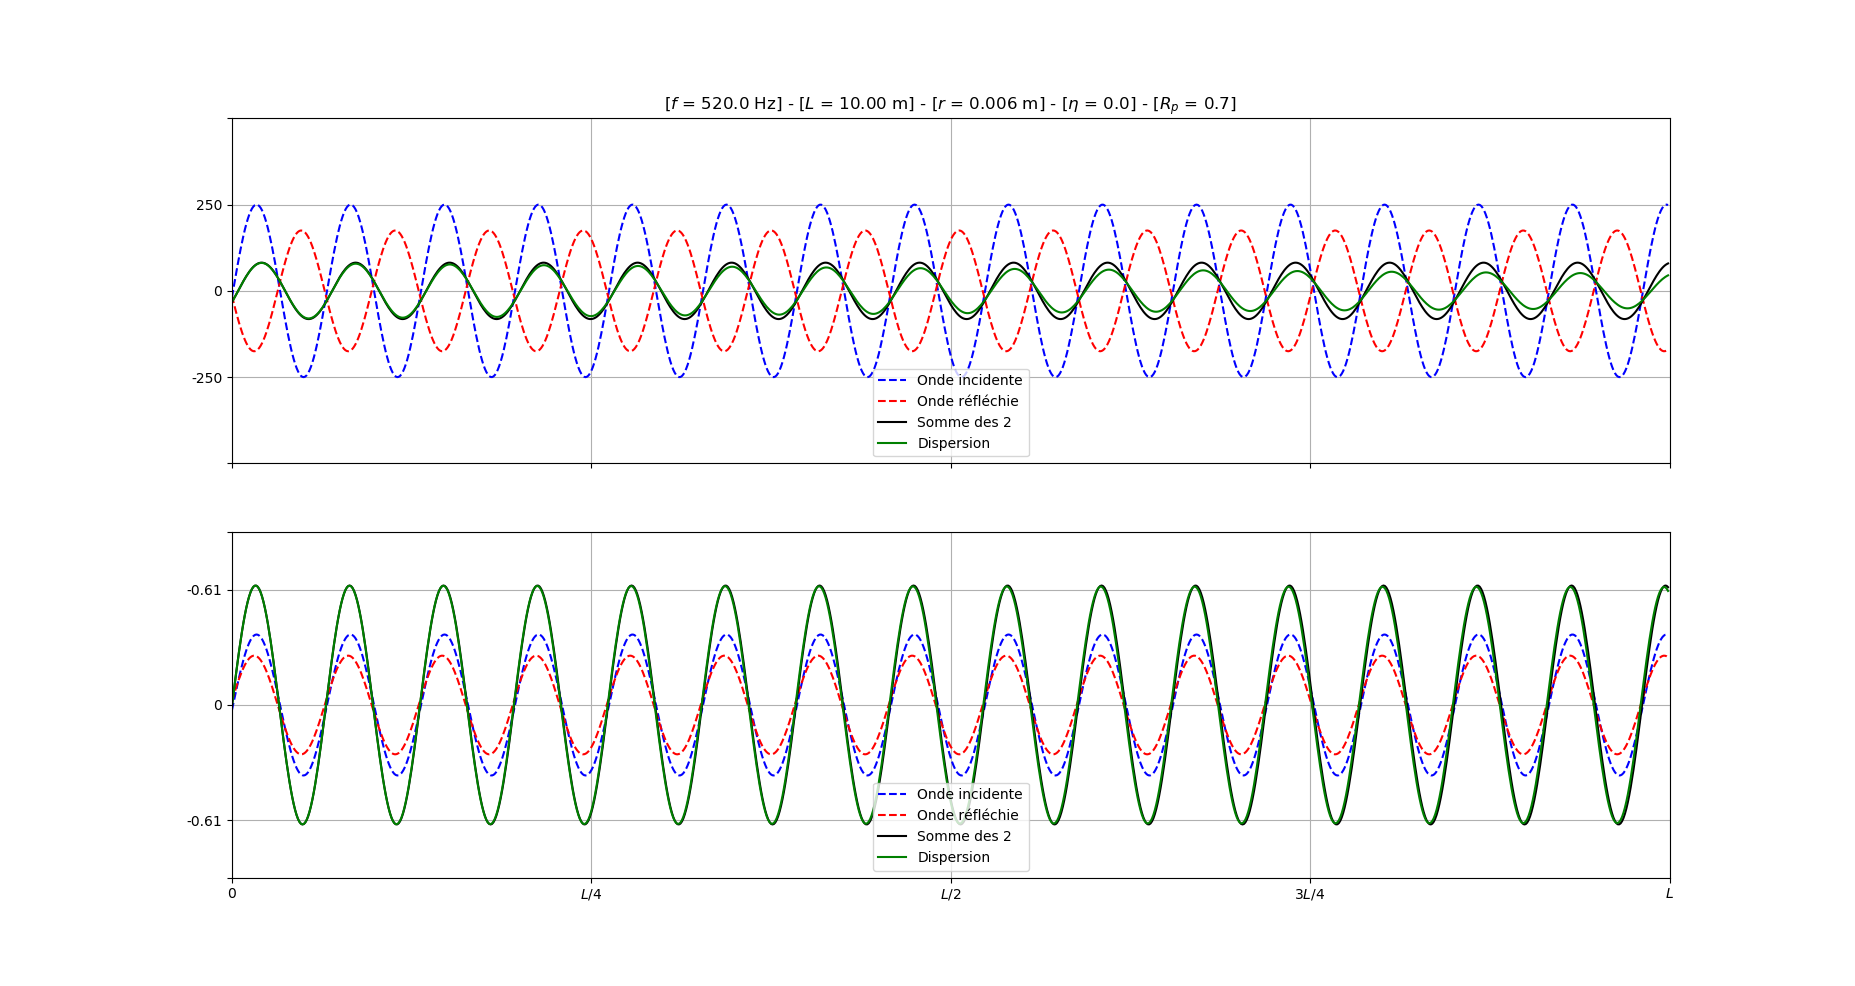
\includegraphics[width=\linewidth]{Figures/tubeKundt_dispers.png}
	\caption{Capture d'écran de la simulation du champ acoustique dans le tube en prenant en compte les phénomènes de pertes}
	\label{fig:simul_acpertes} 
\end{figure}


Cette expression théorique montre, qu'en théorie, il y aura de la dispersion à une fréquence élevée et un rayon faible de la section du tube, soit $r \ll f$. La dissipation aura lieu, quant à elle, quand la longueur du tube est grande et s'il y a des ondes stationnaires: plus l'onde stationnaire se situe sur un minimum de pression, plus l'onde est atténuée. Il est possible de visualiser le phénomène de dispersion sans l'atténuation dans un tube assez court, mais l'atténuation s'accompagne généralement de dispersion.

\begin{figure}[H]
    \centering
    \begin{subfigure}[t]{0.45\linewidth}
    	\centering
		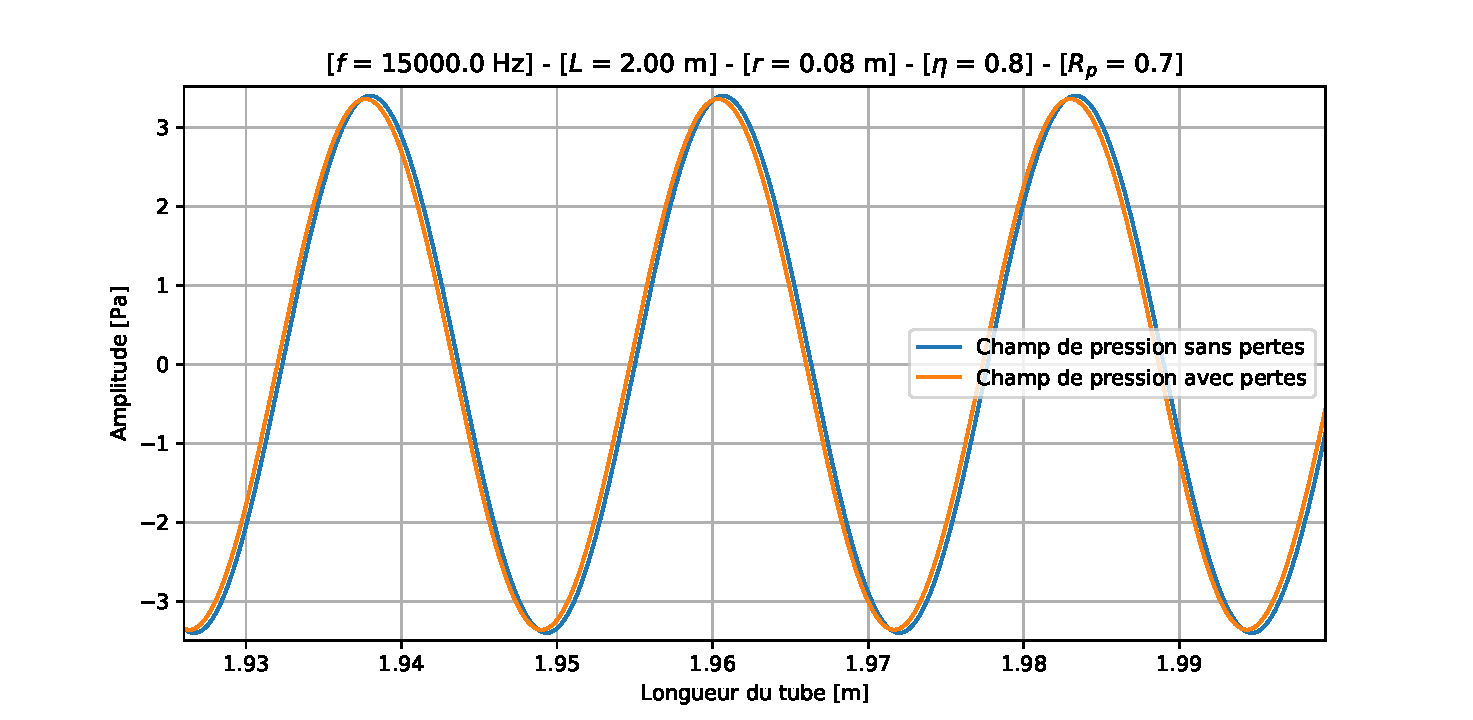
\includegraphics[width=\linewidth]{Figures/dispers.pdf}
		\caption{Dispersion dans un tube}
		\label{fig:dispers} 
    \end{subfigure}
    ~
    \begin{subfigure}[t]{0.45\linewidth}
    	\centering
		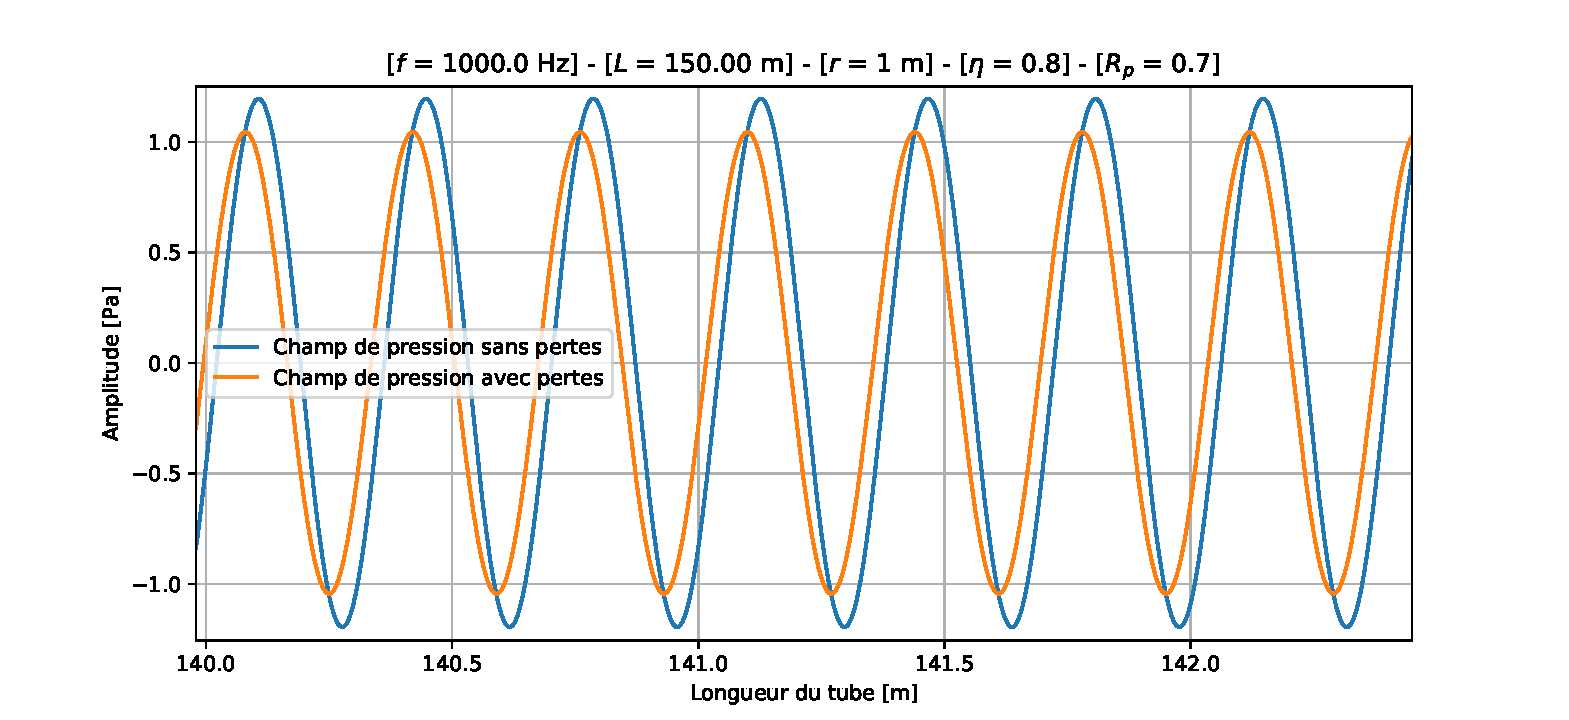
\includegraphics[width=\linewidth]{Figures/atten_dispers.pdf}
		\caption{Atténuation et dispersion du champ acoustique}
		\label{fig:atten_dispers}
    \end{subfigure}
    \caption{Phénomènes de pertes dans différentes configurations pour un tube de Kundt}\label{fig:atten_kundt}
\end{figure}

En observant la figure \ref{fig:dispers}, il est possible de voir, dans un tube court (2m ici) le phénomène de dispersion: l'onde en orange semble déphasée par rapport à l'onde. En fait, sa fréquence est plus faible, du fait de la variation du nombre d'onde avec la fréquence et le rayon du tube: c'est le phénomène de dispersion. Pour observer une atténuation, c'est-à-dire une perte d'énergie, il faut allonger le tube de Kundt: dans la figure \ref{fig:atten_dispers}, le tube mesure 150m et on visualise le champ acoustique avec et sans pertes au bout du tube. Il est possible d'observer une nette diminution de l'amplitude ainsi qu'une forte dispersion: il est impossible de visualiser une atténuation sans dispersion dans ce cas, en utilisant la variation de la célérité de l'onde avec la fréquence.

La simulation numérique du tube de Kundt a permis de mettre en application des connaissances théorique (cours d'acoustique 1D du semestre 3) afin de comprendre visuellement l'évolution du champ acoustique dans ce tube, approfondir le phénomène de pertes et de comprendre de quels facteurs dépend de le coefficient de réflexion.

 Les fichiers utilisés pour ce projet sont: \verb|tubeKundt.py| qui contient l'animation du tube avec la dispersion, \verb|coef_refl| trace le coefficient de réflexion (module, phase, partie réelle et partie imaginaire) et enfin, \verb|tubeKundt_config_dispersion.py| trace la pression dans le tube en prenant en compte l'atténuation et met en évidence ce phénomène.
 
 
 
 


\newpage
\section{L'interface du reste de ma vie}

Pour ce troisième projet, nous allons créer une interface permettant de charger un fichier généré par le logiciel \textit{INTAC} du CTTM et d'afficher les résultats. Pour cela, il s'agit de décomposer le travail en plusieurs étapes: créer les fonctions pour charger un fichier texte, puis le tracer, et ensuite créer une interface utilisateur avec des boutons et un espace d'affichage afin de pouvoir visualiser la courbe et interagir avec pour modifier par exemple l'affichage ou le type de tracé (temporel ou fréquentiel). 

La première étape est assez simple: demander à l'utilisateur le chemin du fichier à charger et le tracer demande seulement quelques lignes en utilisant l'instruction \verb|data = np.loadtxt(filename)| où \verb|filename| est une chaîne de caractères contenant le chemin du fichier texte à charger. Ensuite, il suffit de créer une figure avec matplotlib pour la tracer.

La seconde et principale étape est plus délicate: il faut utiliser un module permettant de créer une interface graphique pour qui utilise ces fonctions. Il existe de nombreux modules qui permettent de créer des GUI (graphical user interface) tels que Tkinter, PyQt, Kivy ou beaucoup d'autres. Mon choix s'est porté sur le module PyQt pour sa simplicité à utiliser avec des classes. La difficulté de ce module reste tout de même que la documentation est en C et non en python, mais de nombreux exemples et tutoriels existent pour prendre en main ce module. Enfin, j'ai choisi ce module car il comprend une intégration plutôt simple de Matplotlib, que ce soit pour la figure ou la barre d'outils.

\subsection{Créer l'interface}

Le programme de l'interface est donc construit sous la forme d'une classe "GUI", initialisée avec des variables précisant la géométrie de la fenêtre, son titre, icône et des variables utiles au fonctionnement des différentes fonctions de l'interface. De façon générale, l'initialisation de cette classe doit comprendre tous les objets que l'on veut afficher dans l'interface. La création des objets et la disposition de ces derniers sont donc séparés dans 2 méthodes différentes appelées dans l'initialisation. Cette classe est de type \verb|QDialog|. Il y a plusieurs types de classe pour créer une interface dont: \verb|QWidget|, \verb|QDialog|, \verb|QMainWindow|. On utilise l'une ou l'autre de ces classes selon l'interface à créer: 
\begin{itemize}
	\item \verb|QMainWindow| permet la création d'une barre de manu, d'une barre d'outils et d'autres objets dont une fenêtre principal peut avoir besoin.
	\item \verb|QDialog| est plus utile pour une petite interface. Elle est basée sur \verb|QWidget| et est designée pour apparaître comme une fenêtre. De plus, elle a des fonctions qui rendent la création de boutons assez basique simple et bien intégrée à la fenêtre.
	\item Enfin \verb|QWidget| est la classe de base pour tout objet affichable sous Qt. Quand un objet widget n'a pas de fenêtre parent, il peut être affiché comme une fenêtre. 
\end{itemize}

Le choix d'utiliser \verb|QDialog| est relativement arbitraire mais est justifié par le fait que pour le développement de cette interface, il nous faut avoir la possibilité de faire afficher une fenêtre "enfant" pour afficher l'arborescence du disque et choisir un fichier à tracer au lieu de devoir chercher le chemin de chaque fichier, c'est l'objectif premier de cette interface. Il n'est pas possible d'ouvrir une boîte de dialogue avec \verb|QWidget|. Enfin, \verb|QMainWindow| paraît un peu exagéré: une barre d'outils/ de menus est inutile pour une interface de cette taille.

\subsubsection{Disposition des éléments dans une fenêtre}

Pour commencer et avant de travailler l'algorithmique derrière l'interface, il s'agit de créer les boutons et les différents espaces de la fenêtre. Pour cela, PyQt possède une fonctionnalité intéressante: les layouts. Les layouts sont des espaces pouvant contenir des objets comme des boutons, un menu déroulant, du texte ou des cases à cocher, permettant d'utiliser un placement relatif pour tous ces objets plutôt qu'une disposition absolue (où chaque bouton est placé selon des coordonnées précises sur la fenêtre). Pour créer la fenêtre initiale, il y a 2 méthodes: la première est de tout faire en ligne de code et à la main. Chaque bouton est ainsi créé, paramétré et placé manuellement dans son layout. Cette méthode est assez longue et rend le programme de l'interface très long et peu lisible. 

Cependant, c'est la seule méthode que je connaissais quand j'ai crée la première version de ce projet, avant de découvrir le logiciel \textit{Qt Designer} qui permet de disposer les layouts et les boutons visuellement. Il suffit ensuite d'importer le fichier que sort le logiciel dans le script et de connecter les boutons aux méthodes associées. Cette seconde méthode est beaucoup rapide et permet de faire des interfaces bien plus esthétiques. De plus, en plaçant correctement les boutons dans un \textit{layout}, la fenêtre s'adapte en cas de redimensionnement.

\begin{figure}[H]
	\centering
	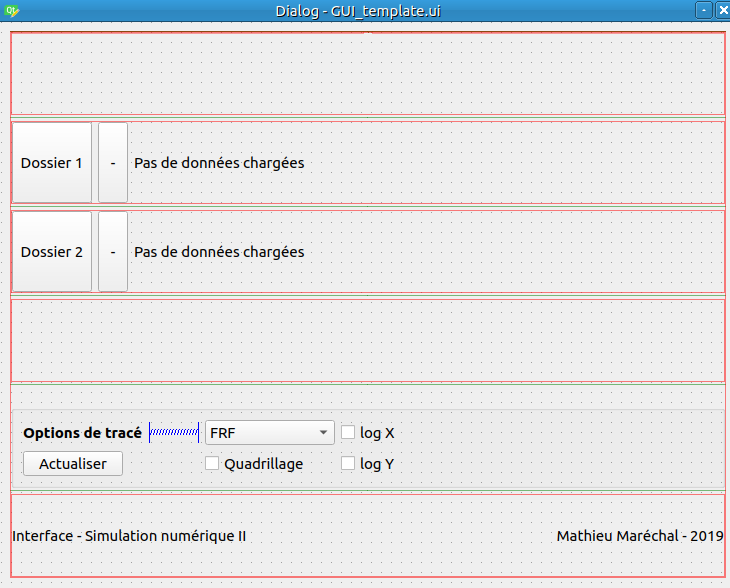
\includegraphics[scale=0.3]{Figures/interf_qt.png}
	\caption{Capture d'écran de l'interface du projet 3 réalisée avec Qt Designer}
	\label{fig:interf_qt} 
\end{figure}

\subsubsection{Chargement de fichiers et tracé de données}

Maintenant que l'interface a tous les boutons nécessaires, il faut les connecter à des méthodes. Pour cela, on utilise \verb|button.clicked.connect(methode)|. Cette ligne permet de lier un bouton à une méthode, qui sera appelée au moment du clic sur le bouton "button". Pour commencer, il faut avoir des fichiers à tracer: on peut, par exemple, ouvrir une boîte de dialogue permettant à l'utilisateur de sélectionner les données à tracer. Les méthodes disponibles avec ce module permettent de proposer de charger un fichier ou un ensemble de fichier avec la méthode \verb|QFileDialog.getOpenFileName()| ou de charger un dossier entier \verb|QFileDialog.getExistingDirectory()|. La première version de l'interface permettait de charger un fichier à la fois, mais la version actuelle prend en charge un dossier complet avec plusieurs types de tracés possible. 

Les méthodes ouvrant une boîte de dialogue retourne le chemin absolu du dossier sous forme d'une chaîne de caractères. Une fois que l'on stocke ce chemin dans une variable, on peut demander à l'utilisateur le type de fichier à charger, puis appeler ce fichier dans la méthode \verb|np.loadtxt| de numpy pour en charger les données. En effet, les dossiers générés par le logiciel du CTTM à l'exportation des mesures comportent des fichiers avec des noms toujours identique: 
\begin{itemize}
	\item pour une acquisition temporelle, \verb|TemporalData.txt|
	\item pour une FRF, \verb|FRF_ModPhase.txt|
	\item pour un spectre, \verb|PowerSpetrum.txt|
\end{itemize}

Cependant, en testant avec des fichiers volumineux, on remarque rapidement que cette méthode est très longue pour charger des fichiers. Une alternative trouvée pour l'importation de fichiers est la méthode \verb|read_csv| du module \verb|pandas|, qui est beaucoup plus rapide. Pour comparer ces 2 méthodes,  j'ai utilisé la fonction \verb|%timeit| de \textit{ipython} et qui permet de mesurer la durée d'exécution d'un programme. Pour un fichier texte de 250 Mo en lisant le fichier texte avec  un SSD, la méthode \verb|np.loadtxt| prend en moyenne $\approx 40$ s à charger le fichier tandis qu'en utilisant la méthode \verb|pd.read_csv|, le temps de chargement du fichier est de 5 sec au plus. La méthode \verb|np.loadtxt| reste intéressante pour des fichiers légers ou pour pouvoir tracer des fichiers rapidement, comme en TP par exemple, mais, dans le cas de cette interface, la rapidité que permet la seconde méthode est très importante et pertinente pour ce programme. Cependant, les chargements de fichiers peuvent quand même prendre du temps. Ainsi, pour éviter tout risque d'erreur, le bouton "Actualiser" est désactivé le temps de l'import du fichier et un label de texte apparaît à droite pour préciser qu'un chargement est en cours.

La méthode \verb|pd.read_csv| retourne donc un ensemble de données du type \verb|DataFrame|. L'avantage de ce type de variable est qu'il permet de retourner le texte de l'en-tête de chaque fichier pour légender les figures à tracer avec l'attribut \verb|DataFrame.axes| et \verb|DataFrame.values| retourne une matrice numpy contenant les données structurées de la même manière que ce que renvoie \verb|np.loadtxt|).

En connaissant les noms de chaque type de fichier créés en sortie du logiciel CTTM, il est possible de créer un menu déroulant détaillant le type de fichiers que l'utilisateur souhaite visualiser et d'importer un fichier précis selon ce choix. Le type de tracé et l'import des fichiers est détaillé dans la méthode 	\verb|loadData| de la classe de l'interface. Après l'appel de cette fonction, les fichiers sont importés, il ne reste plus qu'à tracer les courbes!

La difficulté d'avoir la possibilité de tracer 2 jeux de données en même temps est que, quand l'utilisateur ne veut observer qu'une seule mesure, il faut prendre en compte que seul le dossier 1 ou le dossier 2 contient des données à tracer, et ainsi gérer les erreurs en utilisant des opérateurs booléens renvoyant l'état des différentes étapes comme \verb|loaded_1| et \verb|loaded_2| qui déterminent respectivement si le dossier 1 ou le dossier 2 contient des données à charger. En ajoutant la gestion des erreurs avec les structures \verb|try:| \verb|except|, le programme s'adapte à toutes les conditions possible: selon l'erreur, le programme renvoie un message d'erreur, c'est-à-dire une fenêtre qui s'ouvre et qui précise la source de l'erreur. L'essentiel de la gestion d'erreur est de faire en sorte que l'interface ne se ferme pas à cause d'une erreur. 

Le résultat final est présenté dans une capture d'écran en figure \ref{fig:interf_final}. Des réponses en fréquences de l'excitation d'une plaque en plexiglas par un pot vibrant en 2 points différents mesuré par un accéléromètre sont chargées pour cet exemple.

\begin{figure}[H]
	\centering
	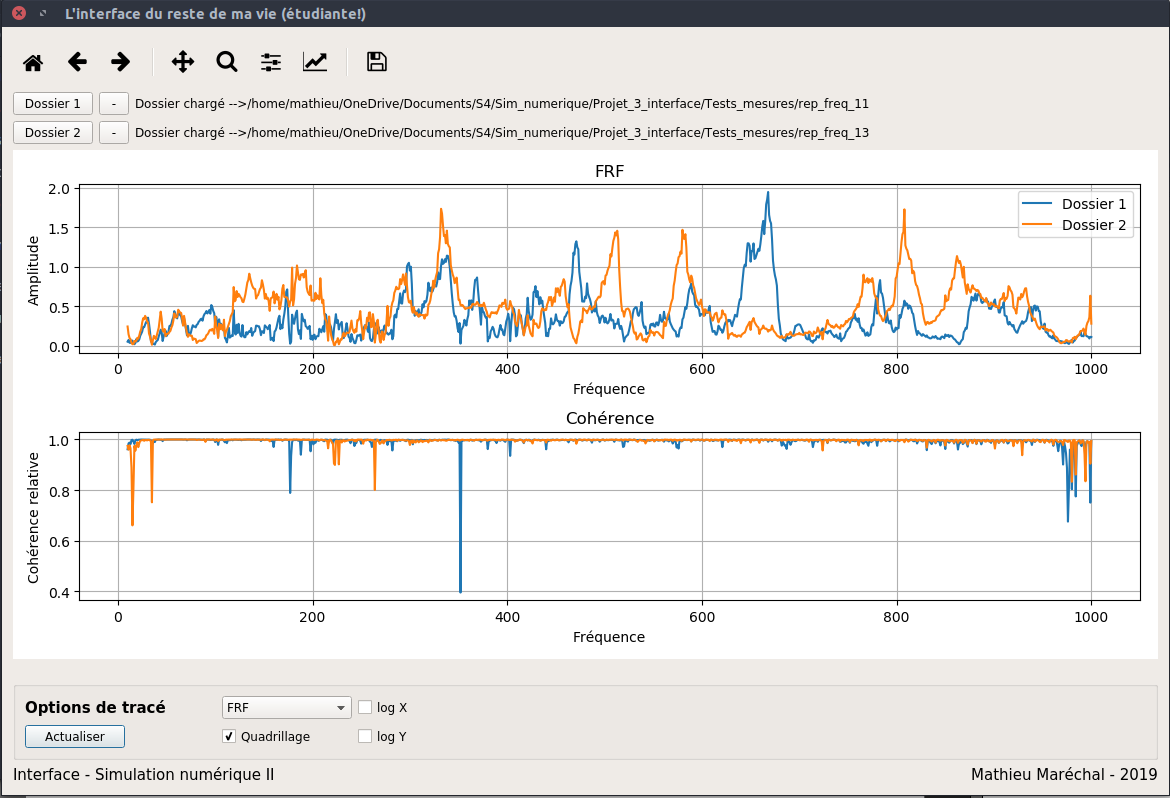
\includegraphics[scale=0.3]{Figures/interf_final.png}
	\caption{Capture d'écran de l'interface final du projet 3}
	\label{fig:interf_final}
\end{figure}

\subsection{Mode d'emploi de l'interface}
Le but de ce programme est de tracer les mesures issues d'acquisitions du logiciel \textit{Analyseur CTTM} exclusivement. Pour commencer, il faut cliquer sur le bouton "Dossier 1" ou "Dossier 2" situé en haut de l'interface. Une boîte de dialogue s'ouvre alors et demande de sélectionner un dossier. Une fois sélectionné, le chemin du fichier s'affiche à droite du bouton. Il faut maintenant sélectionner le mode de tracé souhaité dans la zone "Options de tracé" et ensuite cliquer sur le bouton "Actualiser". Les données peuvent être déchargées du programme en cliquant sur le bouton "-" situé à droite du bouton de chargement. Jusqu'à 2 jeux de données peuvent être chargés à la fois. Finalement, les fonctionnalités proposées par les figures matplotlib classiques sont disponibles ici: zoom, sauvegarde des figures, ...

Les fichiers présentés pour ce projet sont:
\begin{itemize}
	\item un dossier "TestMesures" qui contient des dossiers issus de l'Analyseur CTTM avec différents formats et différentes tailles de fichiers
	\item un fichier \verb|GUI_template|, en \verb|.ui| qui vient du logiciel Qt Designer et qui contient les éléments de l'interface graphique et l'autre en \verb|.py| qui permet d'importer ces éléments dans le script
	\item un fichier \verb|GUI_v1.py| qui est la première version de l'interface graphique sans utiliser le \textit{template}
	\item les deux versions suivantes du projet dans les fichiers \verb|GUI_v2.py| et \verb|GUI_v3.py|. La version finale de ce projet est bien la version 3.	
\end{itemize}



\newpage
\section{Traitement du signal et imagerie}
Ce quatrième projet sur le sujet du traitement de signal: l'objectif est de tracer et traiter de différentes manières un fichier de données puis de traiter un grand nombre de mesure dans une seconde partie. 

\subsection{Traitement du signal acoustique picoseconde}
L'objectif de cette partie est d'apprendre la démarche de réflexion et de traitement à avoir pour extraire des informations d'un signal, quel qu'il soit. Tout d'abord, il s'agit de charger le fichier et de le tracer. Ensuite, il faut calculer le module du spectre (en suivant la méthode détaillée dans le sujet du projet) avec les fonctions \verb|np.fft.ftt| et \verb|np.fft.fftfreq| du module numpy, afin de visualiser le contenu fréquentiel du fichier \verb|time_rawsignals_84GPa_nice.txt|. En prenant en compte le fait que l'axe temporel est gradué en nanosecondes (ns), l'unité de l'axe fréquentiel est en GHz, soit $10^9$ Hz.
Le résultat de cette partie est représenté en figure \ref{fig:tds1}. Le spectre se situe sur la deuxième sous-figure: les données brut sont en bleu. Le contenu fréquentiel est donc principalement situé dans le domaine $[0 - 200]$ GHz. Cependant, en basse fréquence, c'est le pic de coïncidence qui est présent, puisque l'impulsion a une période assez longue par rapport aux oscillations, à la suite du signal. Le spectre montre que le signal est bruité à partir de 250 - 300 GHz. Le contenu fréquentiel situé dans le domaine déterminé précédemment correspond à la fréquence de l'oscillation de Brillouin dans le polycristal de glace d'eau.

\begin{figure}[H]
	\centering
	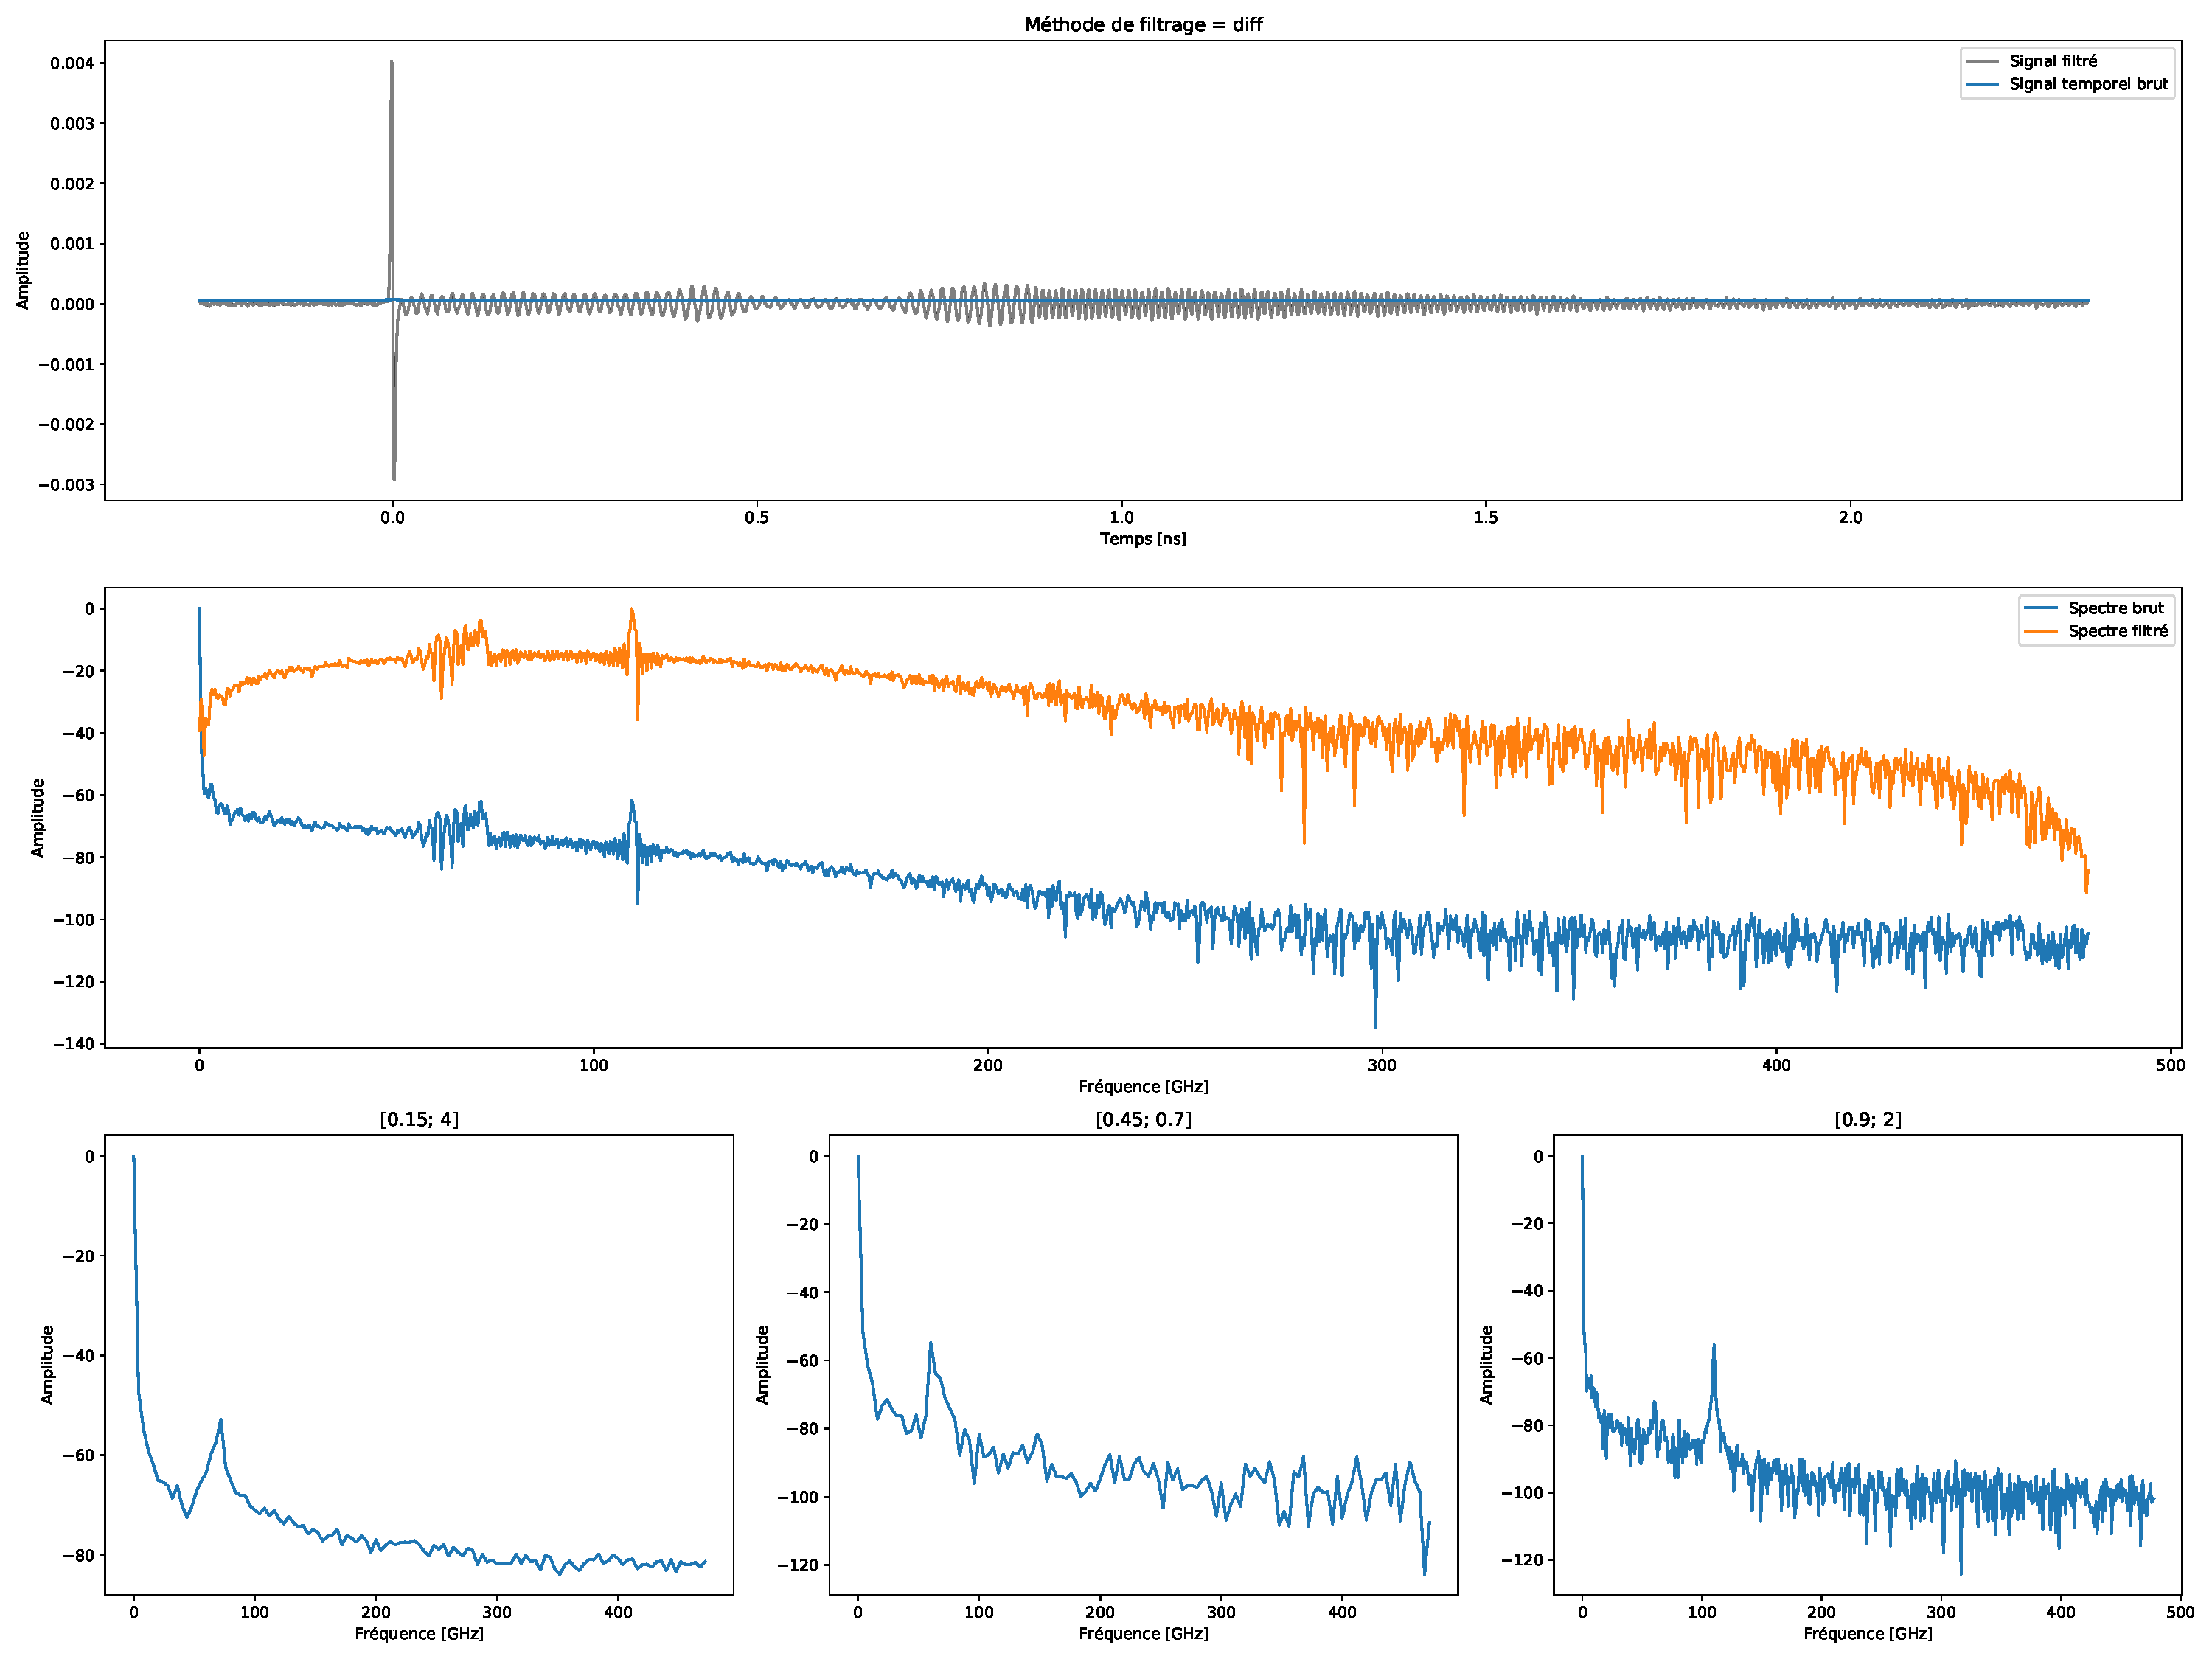
\includegraphics[width=\linewidth]{Figures/TDS1.pdf}
	\caption{Représentation et traitement du signal acoustique picoseconde selon les différentes méthodes demandées avec un filtrage passe-bande}
	\label{fig:tds1}
\end{figure}

\begin{figure}[H]
	\centering
	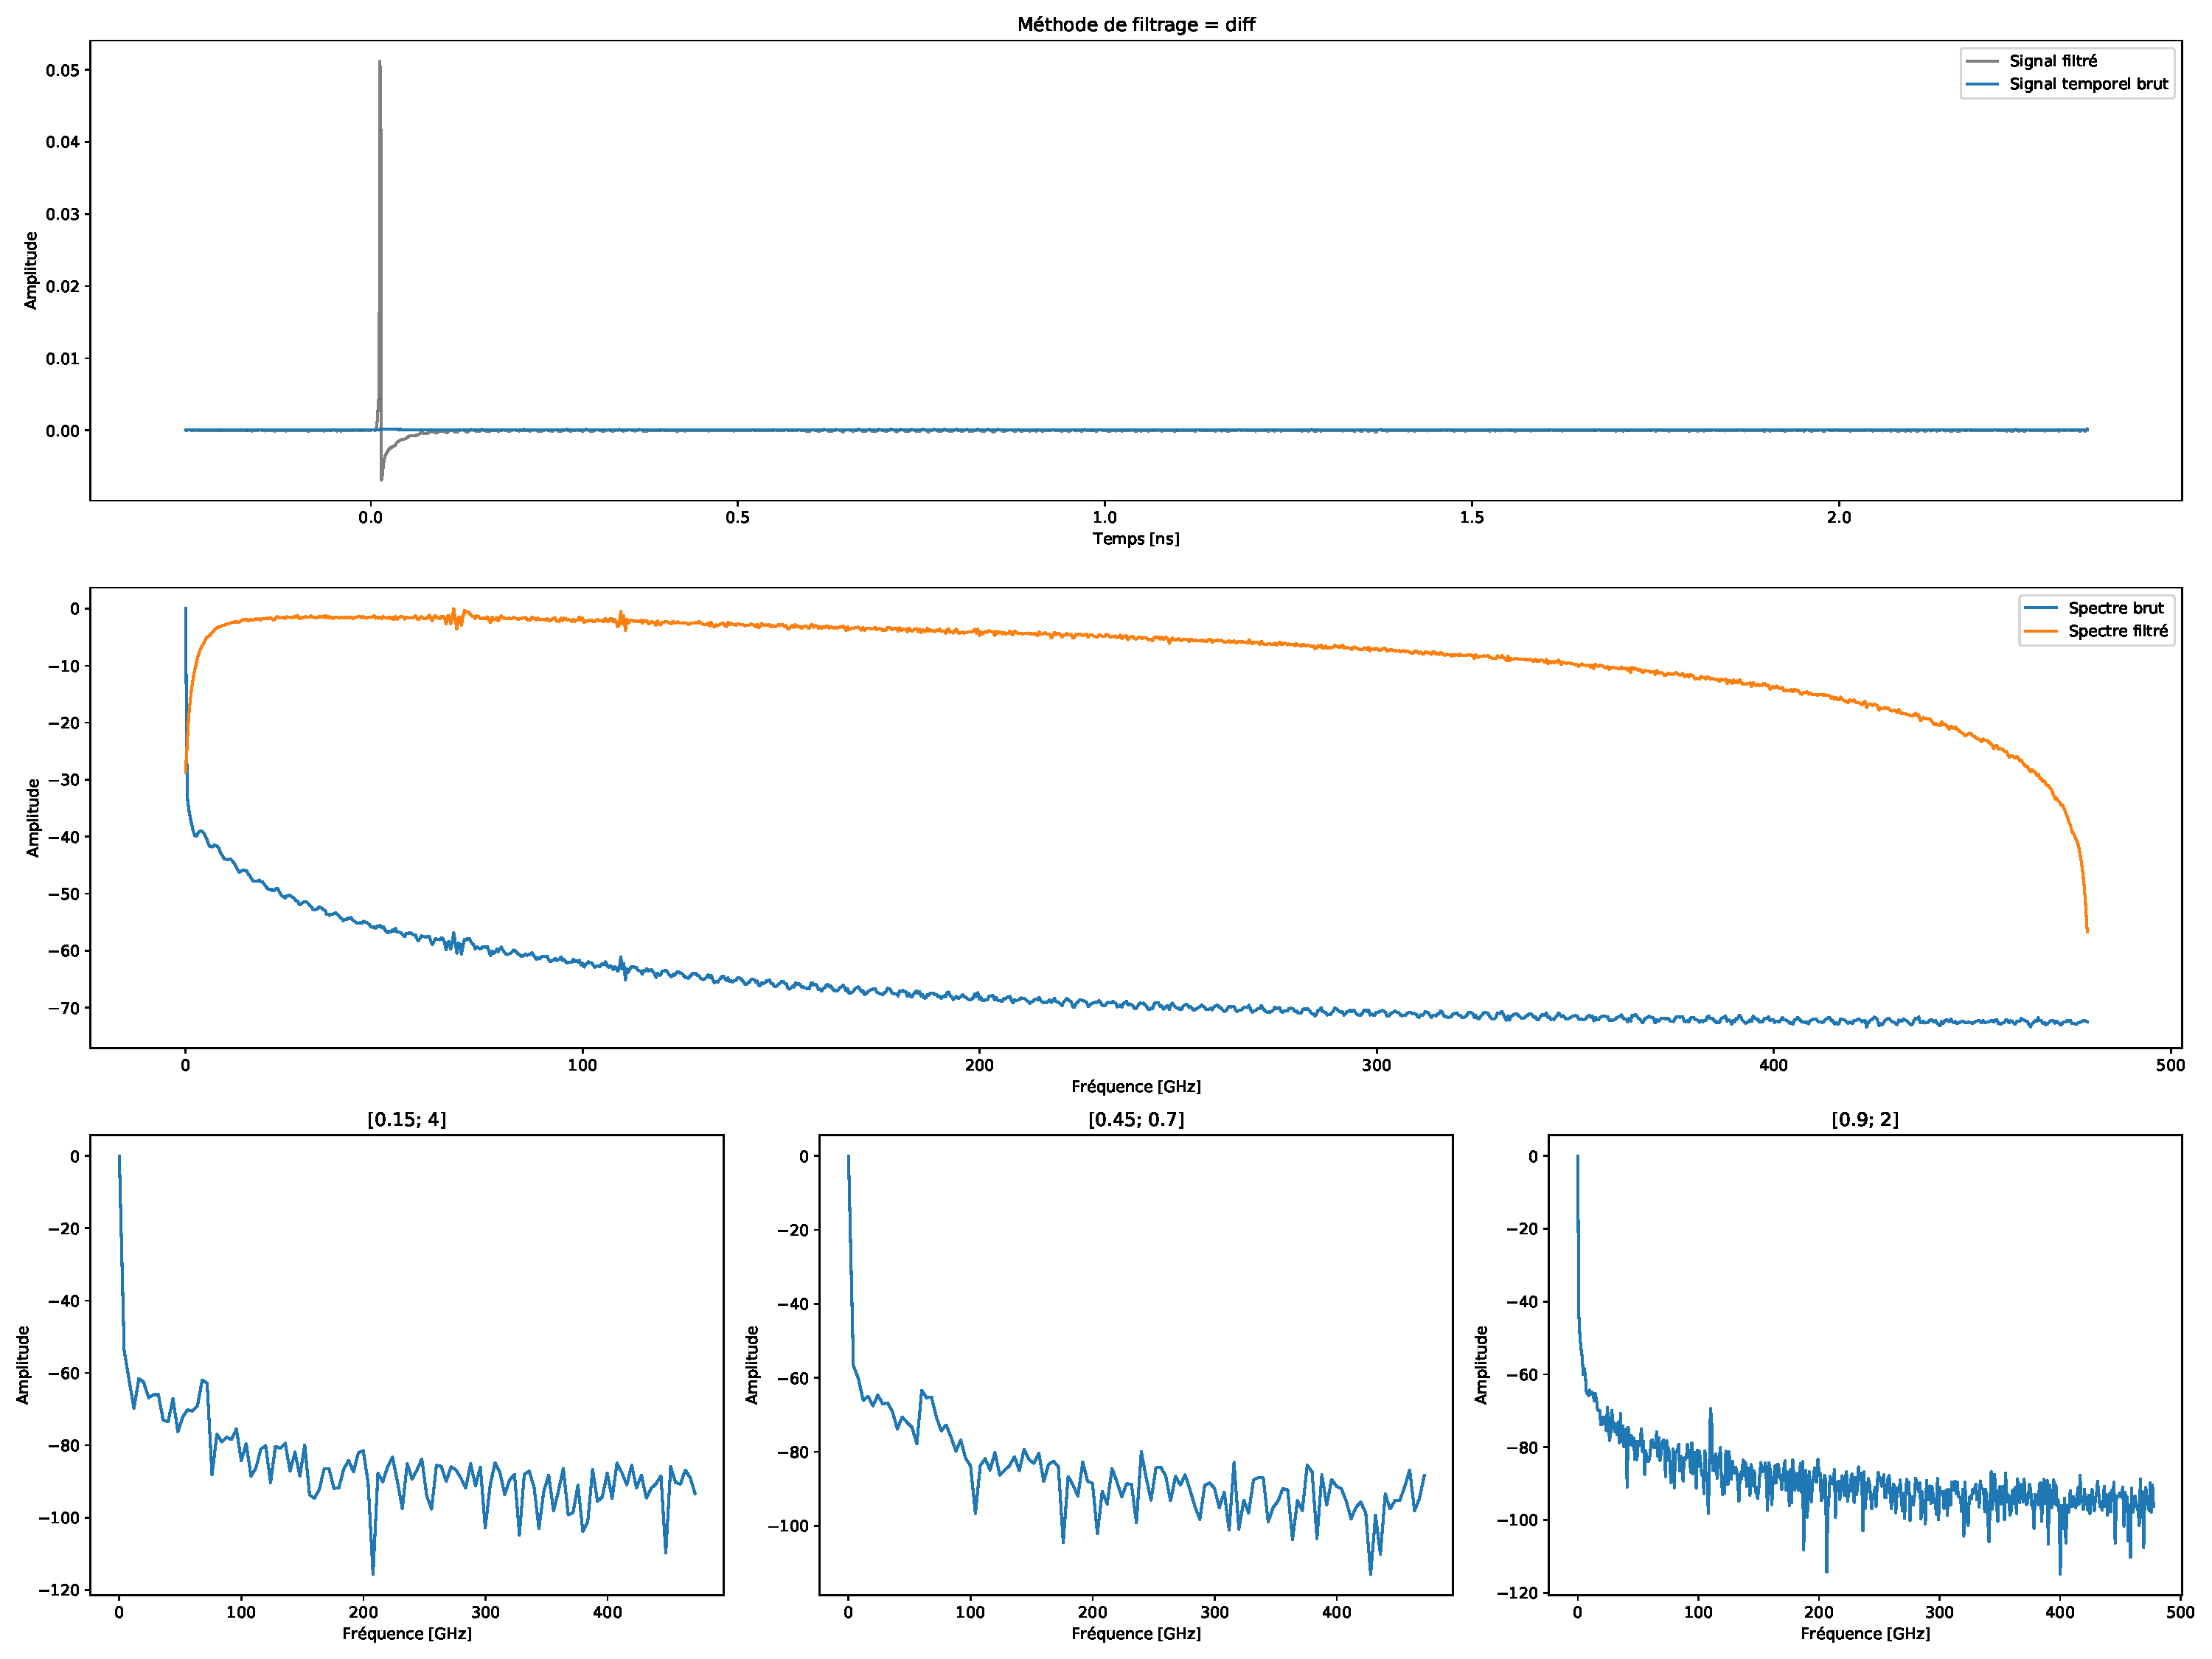
\includegraphics[width=\linewidth]{Figures/TDS1_bad.pdf}
	\caption{Représentation et traitement du signal acoustique picoseconde selon les différentes méthodes demandées avec un filtrage passe-bande}
	\label{fig:tds1_bad} 
\end{figure}

L'étape suivante propose de calculer la FFT sur trois intervalles différents: de 0.15 à 4 ns, de 0.45 à 07 ns et enfin de 0.9 ns à 2.0 ns. Il est alors possible d'observer les fréquences de  résonances sur chaque signal: sur le premier intervalle, la résonance se trouve à environ 80 GHz, sur le 2e, à 60 GHz et à 110GHz sur le dernier échantillon. Ces 3 mesures montrent l'évolution de la fréquence de résonance avec le temps.

Avec le signal \verb|time_rawsignals_84GPa_bad.txt.|, la même figure que précédemment est tracée. il est visible que les données contenues dans ce fichier sont similaires mais présente une différence importante: après le pic d'excitation, les oscillations sont très faibles, ce qui rend le signal peut exploitable: la différence entre le signal \verb|nice| et \verb|bad| est que le signal bad a une impulsion dont l'amplitude est bien plus élevée.

On constate qu'avec les 2 signaux tracés précédemment, les fréquences de résonances n'apparaissent pas clairement: l'amplitude du pic est faible, tout comme au niveau du tracé temporel où les oscillations suivant le pic au début du signal sont faibles par rapport à ce pic. Pour faire ressortir le pic de résonance, une méthode de filtrage peut être appliquée à la mesure avant le calcul de la FFT. 

\subsection{Filtrage du signal}
Dans le cas de cette mesure, utiliser un filtrage sera utile afin de supprimer les basses fréquences de ce signal. Nous allons donc voir plusieurs méthodes pour appliquer numériquement un filtre basse-fréquence. Toutes ces méthodes peuvent être comparées avec la figure présentée en annexe A.

\subsubsection{Dérivée du signal}
Pour filtrer les basses fréquences, une première méthode peut consister à calculer numériquement la dérivée du signal. Pour cela, il est commun d'utiliser la formule du taux d'acroissement qui donne la dérivée:
\begin{equation}
	f'(a) = \lim_{h \rightarrow 0} \frac{f(a + h) - f(a)}{h}
\end{equation}
Cette méthode ayant déjà été implémentée au cours d'un TP au S2, le code a été réutilisé pour cette méthode de filtrage. La dérivation permet effectivement de filtrer les basses-fréquences, car dériver un signal du type $f(x, t) = g(x) e^{j \omega t}$, c'est-à-dire dépendant du temps, revient en fait à le multiplier par $j \omega$. Or, quand $\omega \rightarrow 0$, $f(x, t) \rightarrow 0$. Seulement, pour un pic ayant une pente très élevée, l'allure de la dérivée résulte en un pic avec une amplitude plus élevée, donc il est impossible de filtrer une impulsion avec cette méthode, comme l'illustre la figure en annexe A. Cependant, en regardant le spectre, les fréquences de résonances sont bien mises en évidence.

\subsubsection{Filtrage passe-bande}
La seconde méthode consiste à utiliser une méthode de filtrage passe-bande fournie par le module \textit{SciPy}. La fonction utilisée est \verb|signal.butter| et permet de calculer les coefficients nécessaires à l'application d'un filtre de Butterworth, qui est un filtre linéaire avec une réponse en fréquence très plate. Pour cela, il suffit d'entrer en argument l'ordre du filtre souhaité, le mode de filtrage, ici "bandpass", ainsi. Ensuite, les coefficients sont exploités par la fonction \verb|signal.filtfilt| dans laquelle on précise les 2 coefficients calculés précédemment et le vecteur/liste auquel on doit l'adapter. Le résultat est encore une fois présenté en annexe et la spectre obtenu avec ce traitement met en évidence les fréquences de résonances sur la bande-passante du filtre (40 à 150 GHz). L'avantage par rapport à la méthode précédente est que les hautes fréquences ne sont pas bruitées: le tracé apparaît très linéaire au-dessus de 280 GHz.

\subsubsection{Moyenne glissante}
Une autre méthode de filtrage permettant de supprimer les composantes basses-fréquences du signal est la moyenne glissante. Une fenêtre centrée sur chaque point est sélectionné et la valeur de chacun de ces points est la moyenne de cette fenêtre. La méthode est très simple à implémenter, mais il faut prendre en compte les premiers et derniers points. Pour cela, le choix retenu est d'utiliser une fenêtre pour calculer un point $i$ dont le point est situé à gauche de la fenêtre pour les points ayant un indice inférieur à la largeur de la fenêtre et situé à droite pour les points situés à droite du signal. Dans ce cas, la largeur de la fenêtre sélectionnée est de 40 points. Cette méthode conserve l'allure du signal, qui semble très similaire au signal brut. Cependant, en traçant le spectre, les fréquences de résonances sont moins visibles que pour les traitements précédents et le filtre basse-fréquence est peu efficace puisque l'amplitude maximale du spectre se situe toujours en très basses fréquences.
  
\subsubsection{Ajustements: polynomiale \& exponentielle décroissante}
Les 2 méthodes restantes consistent à ajuster le signal selon des courbes définies mathématiquement: ici un polynôme de degré 80 et une exponentielle décroissante. Ces méthodes sont efficaces pour des signaux simples et l'avantage est que l'implémentation de ces méthodes est très simple mais dans ce cas, elles apparaissent totalement inefficaces: les fréquences de résonances disparaissent totalement, le filtrage est plutôt efficace en basse-fréquences.

\subsection{Image de fréquence Brillouin}
Cette partie consiste à exploiter d'autres fichiers en utilisant les méthodes mises en place précédemment. Dans ce cas, il s'agit de tracer l'image des fréquences Brillouins pour l'échantillon, quand il y a excitation par le laser de génération. Cette image de fréquence contient la fréquence de résonance de l'échantillon selon la position (x, y) de l'excitation laser. Les fréquences Brillouin d'un milieu sont mesurées en excitant un matériau et en identifiant le décalage fréquentiel de la lumière ainsi diffusée. La mesure de ce décalage permet d'identifier certaines propriétés d'un matériau, ou peut être aussi un outil de contrôle non destructif.

Le processus de traitement contient alors: le chargement de chacun des 3600 fichiers, l'extraction de la fréquence de résonance et le stockage de celui-ci dans une matrice qu'on tracera par la suite pour obtenir le résultat présenté en figure \ref{fig:tds2}. Le nommage des fichiers est du type \verb|Image/x_y.txt| où x et y sont les positions en x,y de la mesure. Les fichiers peuvent donc être importés via une double boucle \verb|for|. Ensuite, on remarque certains de ces fichiers ont une amplitude constante de -1000: il faut donc tracer ces points en blanc, c'est-à-dire leur attribuer la valeur \verb|None|. Finalement, la fréquence de résonance peut être extraite en identifiant pour quelle fréquence l'amplitude du spectre est maximale sur l'intervalle souhaité, ici entre 57 GHz et 73 GHz.

\begin{figure}[H]
	\centering
	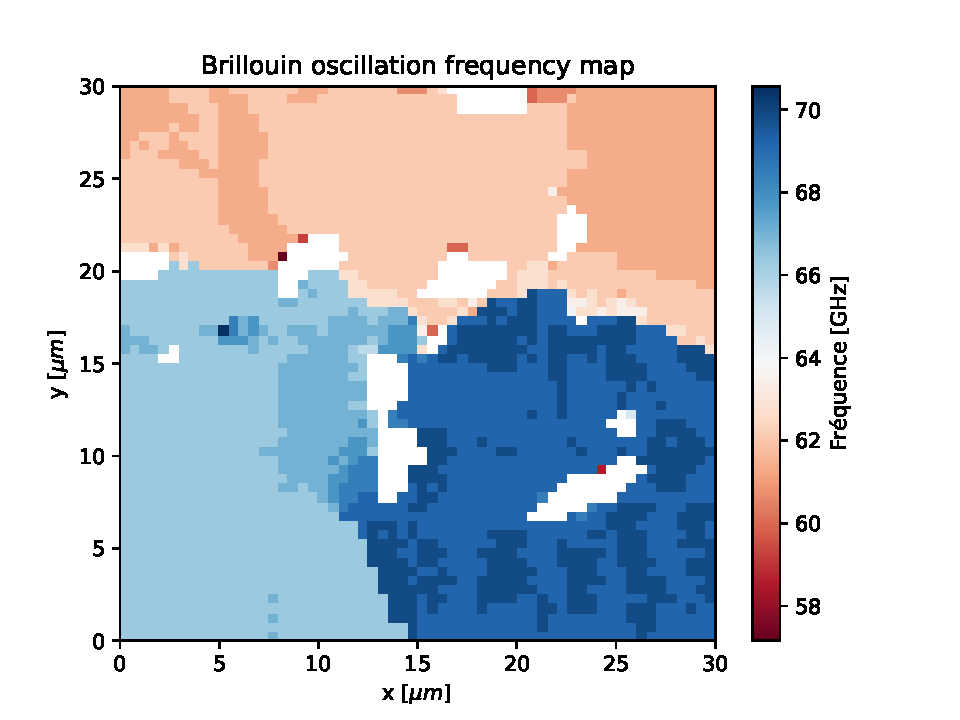
\includegraphics[scale=0.8]{Figures/Brillouin_freq_map.pdf}
	\caption{Image de fréquence Brillouin}
	\label{fig:tds2} 
\end{figure}

La subtilité de cette partie est de déterminer le pas fréquentiel des signaux à traiter: en effet, à cause de la méthode de mesure par échantillonnage optique asynchrone, qui mesure le signal coup après coup, le taux d'échantillonnage ne dépend pas seulement de l'écart entre chaque point mais aussi du décalage entre la répétition du laser de génération et de détection, de la fréquence du laser et de la fréquence d'échantillonnage sélectionnée lors de l'acquisition du signal. Finalement, en remplissant une matrice avec chaque fréquence de résonance identifiée selon sa position, on obtient la cartographie des fréquences pour l'échantillon mesuré, en figure \ref{fig:tds2}.\\

Dans le dossier de ce projet, on retrouve les fichiers:
\begin{itemize}
	\item \verb|TDS.py| qui contient les 3 premières parties du projet
	\item \verb|TDS_MethFiltrage.py| qui trace l'évolution temporel du fichier "bad" ou "nice" ainsi que son spectre avec toutes les méthodes de filtrage implémentées dans le fichier principal
	\item \verb|TDS_part4.py| qui importe les fichiers du dossier "Image" et trace l'image des fréquences Brillouin.
\end{itemize}





\newpage
\section{Optique géométrique}
Pour ce cinquième et dernier projet, il est demandé de mettre en évidence le stigmatisme de différents systèmes optiques. il s'agit de partir de notions d'optique géométrique pour démontrer les conditions menant à un stigmatisme approché et un système non stigmatique. Un système optique est dit stigmatique quand les rayons sortants de ce système convergent en un point précis (ou un ensemble de points très localisée dans le cadre d'un stigmatisme approché (le stigmatisme rigoureux n'existe que théoriquement, pour la réflexion d'un objet sur un miroir plan). Si le système est non-stigmatique, la convergence des rayons en sortie formera une tâche.

L'objectif de ce projet est donc de mettre en évidence ce phénomène pour: les miroirs sphérique concave et convexe et les lentilles sphériques biconcave et biconvexe. Les dioptres seront caractérisés par leur sommet (noté $a$), leur rayon, noté $r$ ainsi que leur diamètre d'ouverture ou épaisseur, notée $e$.

Par la suite, en réfléchissant aux différentes étapes du problème, j'ai réalisé que la difficulté de ce projet n'est pas de nature algorithmique mais géométrique. En effet, pour calculer la trajectoire de rayons lumineux à travers ces lentilles et miroirs, il s'agit d'abord d'établir des relations géométriques donnant la trajectoire de ces rayons. En implémentant ces trajectoires, il ne reste plus qu'à tracer les systèmes optiques avec les rayons associés.

\subsection{Equations de la trajectoire d'un rayon lumineux}
Tout d'abord, il s'agit de tracer les différents éléments optique. Tous les éléments pour lesquels les conditions de stigmatisme sont à illustrer sont constitués d'un ou plusieurs dioptre, qui est soit concave, soit convexe. Pour déterminer toutes les relations mathématiques et géométrique nécessaire au calcul de la trajectoire des rayons, des schémas sont présentés en figure \ref{fig:schema_lentilles}. Il est possible de réaliser les calculs de trajectoires pour ces 2 objets seulement et d'en déduire tous les autres à partir des relations mathématiques et géométrique établies pour ces 2 lentilles. Pour cela, des schémas sont présentés en figure \ref{fig:schema_lentilles}.

Tout d'abord, il s'agit d'établir l'équation décrivant la portion de cercle du dioptre en question. L'équation est donc, à partir de l'équation cartésienne du cercle,
\begin{equation}
	x(y) = \sqrt{r^2 - y^2} - r + e
\end{equation}
puisque l'origine du repère considéré est placé au niveau du point minimum du dioptre (sur l'axe horizontal), la portion de cercle est décalée de $-r+e$. Pour obtenir l'arc de cercle (en bleu sur les schémas), $y$ est un vecteur qui varie de $-a$ à $a$.

\begin{figure}[H]
    \centering
    \begin{subfigure}[t]{0.45\linewidth}
    	\centering
		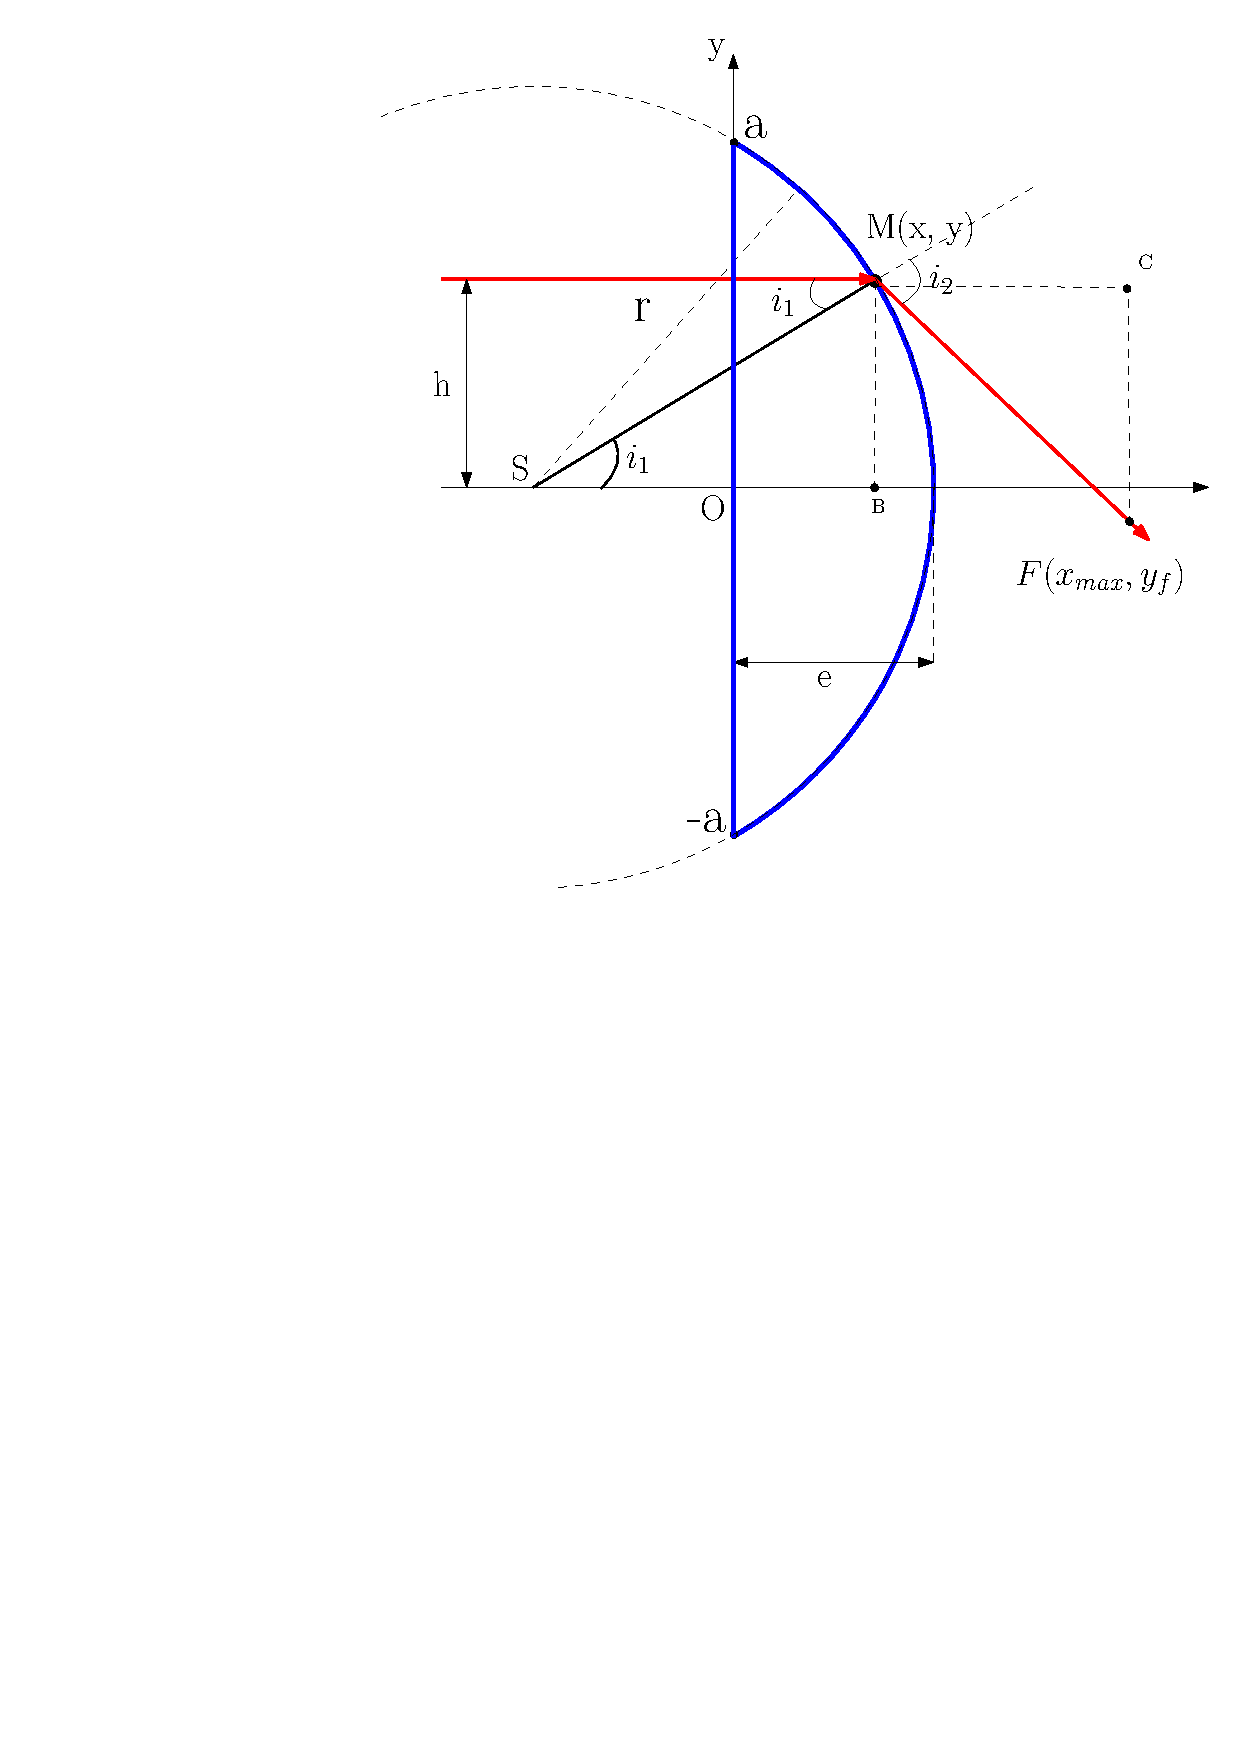
\includegraphics[width=0.8\linewidth]{Figures/schema_lent_conv.pdf}
		\caption{Dioptre convergent (convexe)}
		\label{fig:schema_lent_conv} 
    \end{subfigure}
    ~
    \begin{subfigure}[t]{0.45\linewidth}
    	\centering
		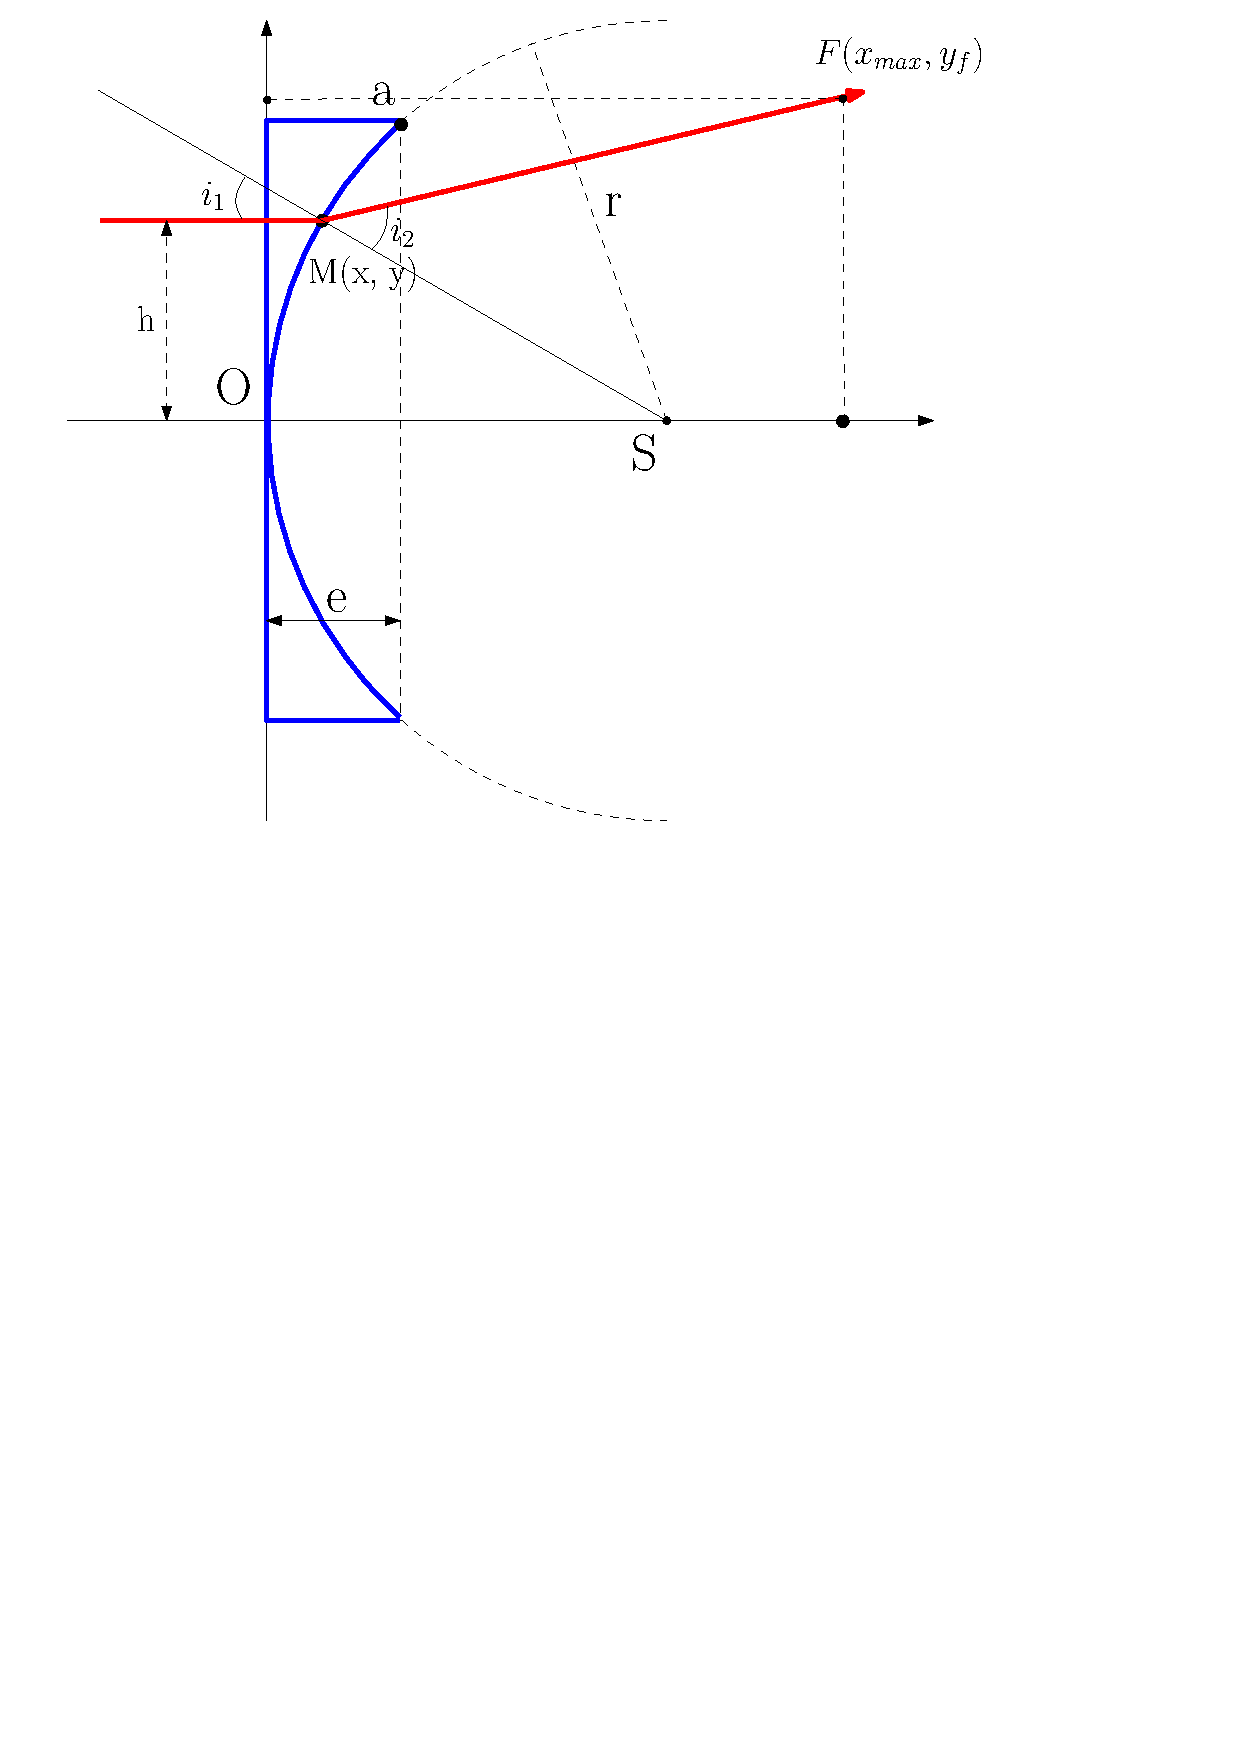
\includegraphics[width=0.8\linewidth]{Figures/schema_lent_div.pdf}
		\caption{Dioptre divergent (concave)}
		\label{fig:schema_lent_div} 
    \end{subfigure}

    \caption{Schémas et notations pour les 2 types de dioptres, ici des lentilles}\label{fig:schema_lentilles}
\end{figure}

\subsubsection{Trajectoire des rayons pour une lentille convergente}
Pour connaître la trajectoire des rayons dans ce cas, le schéma de la figure \ref{fig:schema_lent_conv} est utilisé. Le schéma permet de remarquer que seulement 3 points sont nécessaire pour tracer un rayon: le point d'origine (considéré à l'infini), le point d'intersection sur le dioptre et le point à l'infini vers les x croissants. Dans le programme, deux listes seront alors déclarées:
\begin{verbatim}
	x = [-lim, x_m, lim]
	y = [h, h, y_f]
\end{verbatim}
avec $h$, la hauteur initiale du rayon et \verb|lim|, la limite du domaine. On tracera par la suite les rayons entre $x_{min} = -200$ et $x_{max} = 200$, donc \verb|lim = 200|. Il faut donc maintenant calculer $x_m$ et $y_f$.


En considérant le triangle SBM, il est possible d'établir une relation afin de déterminer $x_m$. Pour cela, le point B est posé et a pour coordonnées $(x_m, 0)$, c'est-à-dire que OB = $x_m$. Il apparaît que SB = $r$ cos $i_1$. Or, SB = $r - e$ + OB. 
Finalement, 
\begin{equation*}
	x_m = r \text{cos}(i_1) - r + e
\end{equation*}

Pour calculer la hauteur du point F, on pose un point C représenté sur le schéma, et on considère le triangle MCF. l'angle en M vaut ici $i_2 - i_1$. Il vient donc que: tan($i_2 - i_1$) = $\frac{CF}{MC}$. Or, MC = $x_{max} - x_m$ et CF = $y_f - h$. Finalement, il vient que:
\begin{equation*}
	y_f = h - (x_{max} - x_m) \: \text{tan} (i_2 - i_1)
\end{equation*}


Enfin, d'après la loi de Snell-Descartes, $\text{sin}(i_1) = n \text{sin}(i_2)$, avec n, l'indice de réfraction du matériau. Or, $i_1 = \text{arcsin}\big( \frac{h}{r}\big)$, donc $i_2 = \text{arcsin}\big( n \frac{h}{r}\big)$

\subsubsection{Trajectoire des rayons pour une lentille divergente}
Pour une lentille divergente, les calculs sont identiques mais comme le rayon réel diverge de l'axe optique, $y_f$ s'exprime comme étant $y_f = h + (x_{max} - x_m) \: \text{tan} (i_2 - i_1)$,
c'est-à-dire que le rayon a une pente positive au lieu d'une pente négative comme le cas d'une lentille convergente, ce qui est logique avec la représentation visuelle. L'autre point à exprimer dans ce cas, est la trajectoire du rayon virtuel réfléchi. Cependant ce rayon a la trajectoire inverse du rayon divergent réel, donc le tracé ne pose pas de problème: on pourra déclarer la hauteur du rayon virtuel réfléchi comme \verb|y_refl = -y_f|.

\subsection{Simulation de la trajectoire de rayons lumineux dans un système optique}
Pour cette dernière étape, il reste à créer le programme. L'idée est de créer 2 classes, une pour les miroirs et l'autres pour les lentilles. 

\subsubsection{Miroirs sphériques concave et convexe}
La classe \verb|Miroir| est très simple: les variables d'initialisation sont le rayon du miroir, son sommet, son épaisseur ainsi que l'équation du miroir sphérique. Ensuite, une méthode \verb|concave| retourne une liste contenant l'équation x en fonction du vecteur y et la méthode \verb|convexe| retourne l'équation opposée: le dioptre divergent est symétrique au dioptre convergent par rapport à l'axe $y=0$, ce qui sera aussi utile au moment de créer une lentille biconvexe. Après avoir pris en compte cette opération, il faut noter que le point $x_m$ désignant le point d'impact du rayon sur la surface du dioptre sera opposé lui aussi.

\begin{figure}[H]
    \centering
    \begin{subfigure}[t]{0.45\linewidth}
    	\centering
		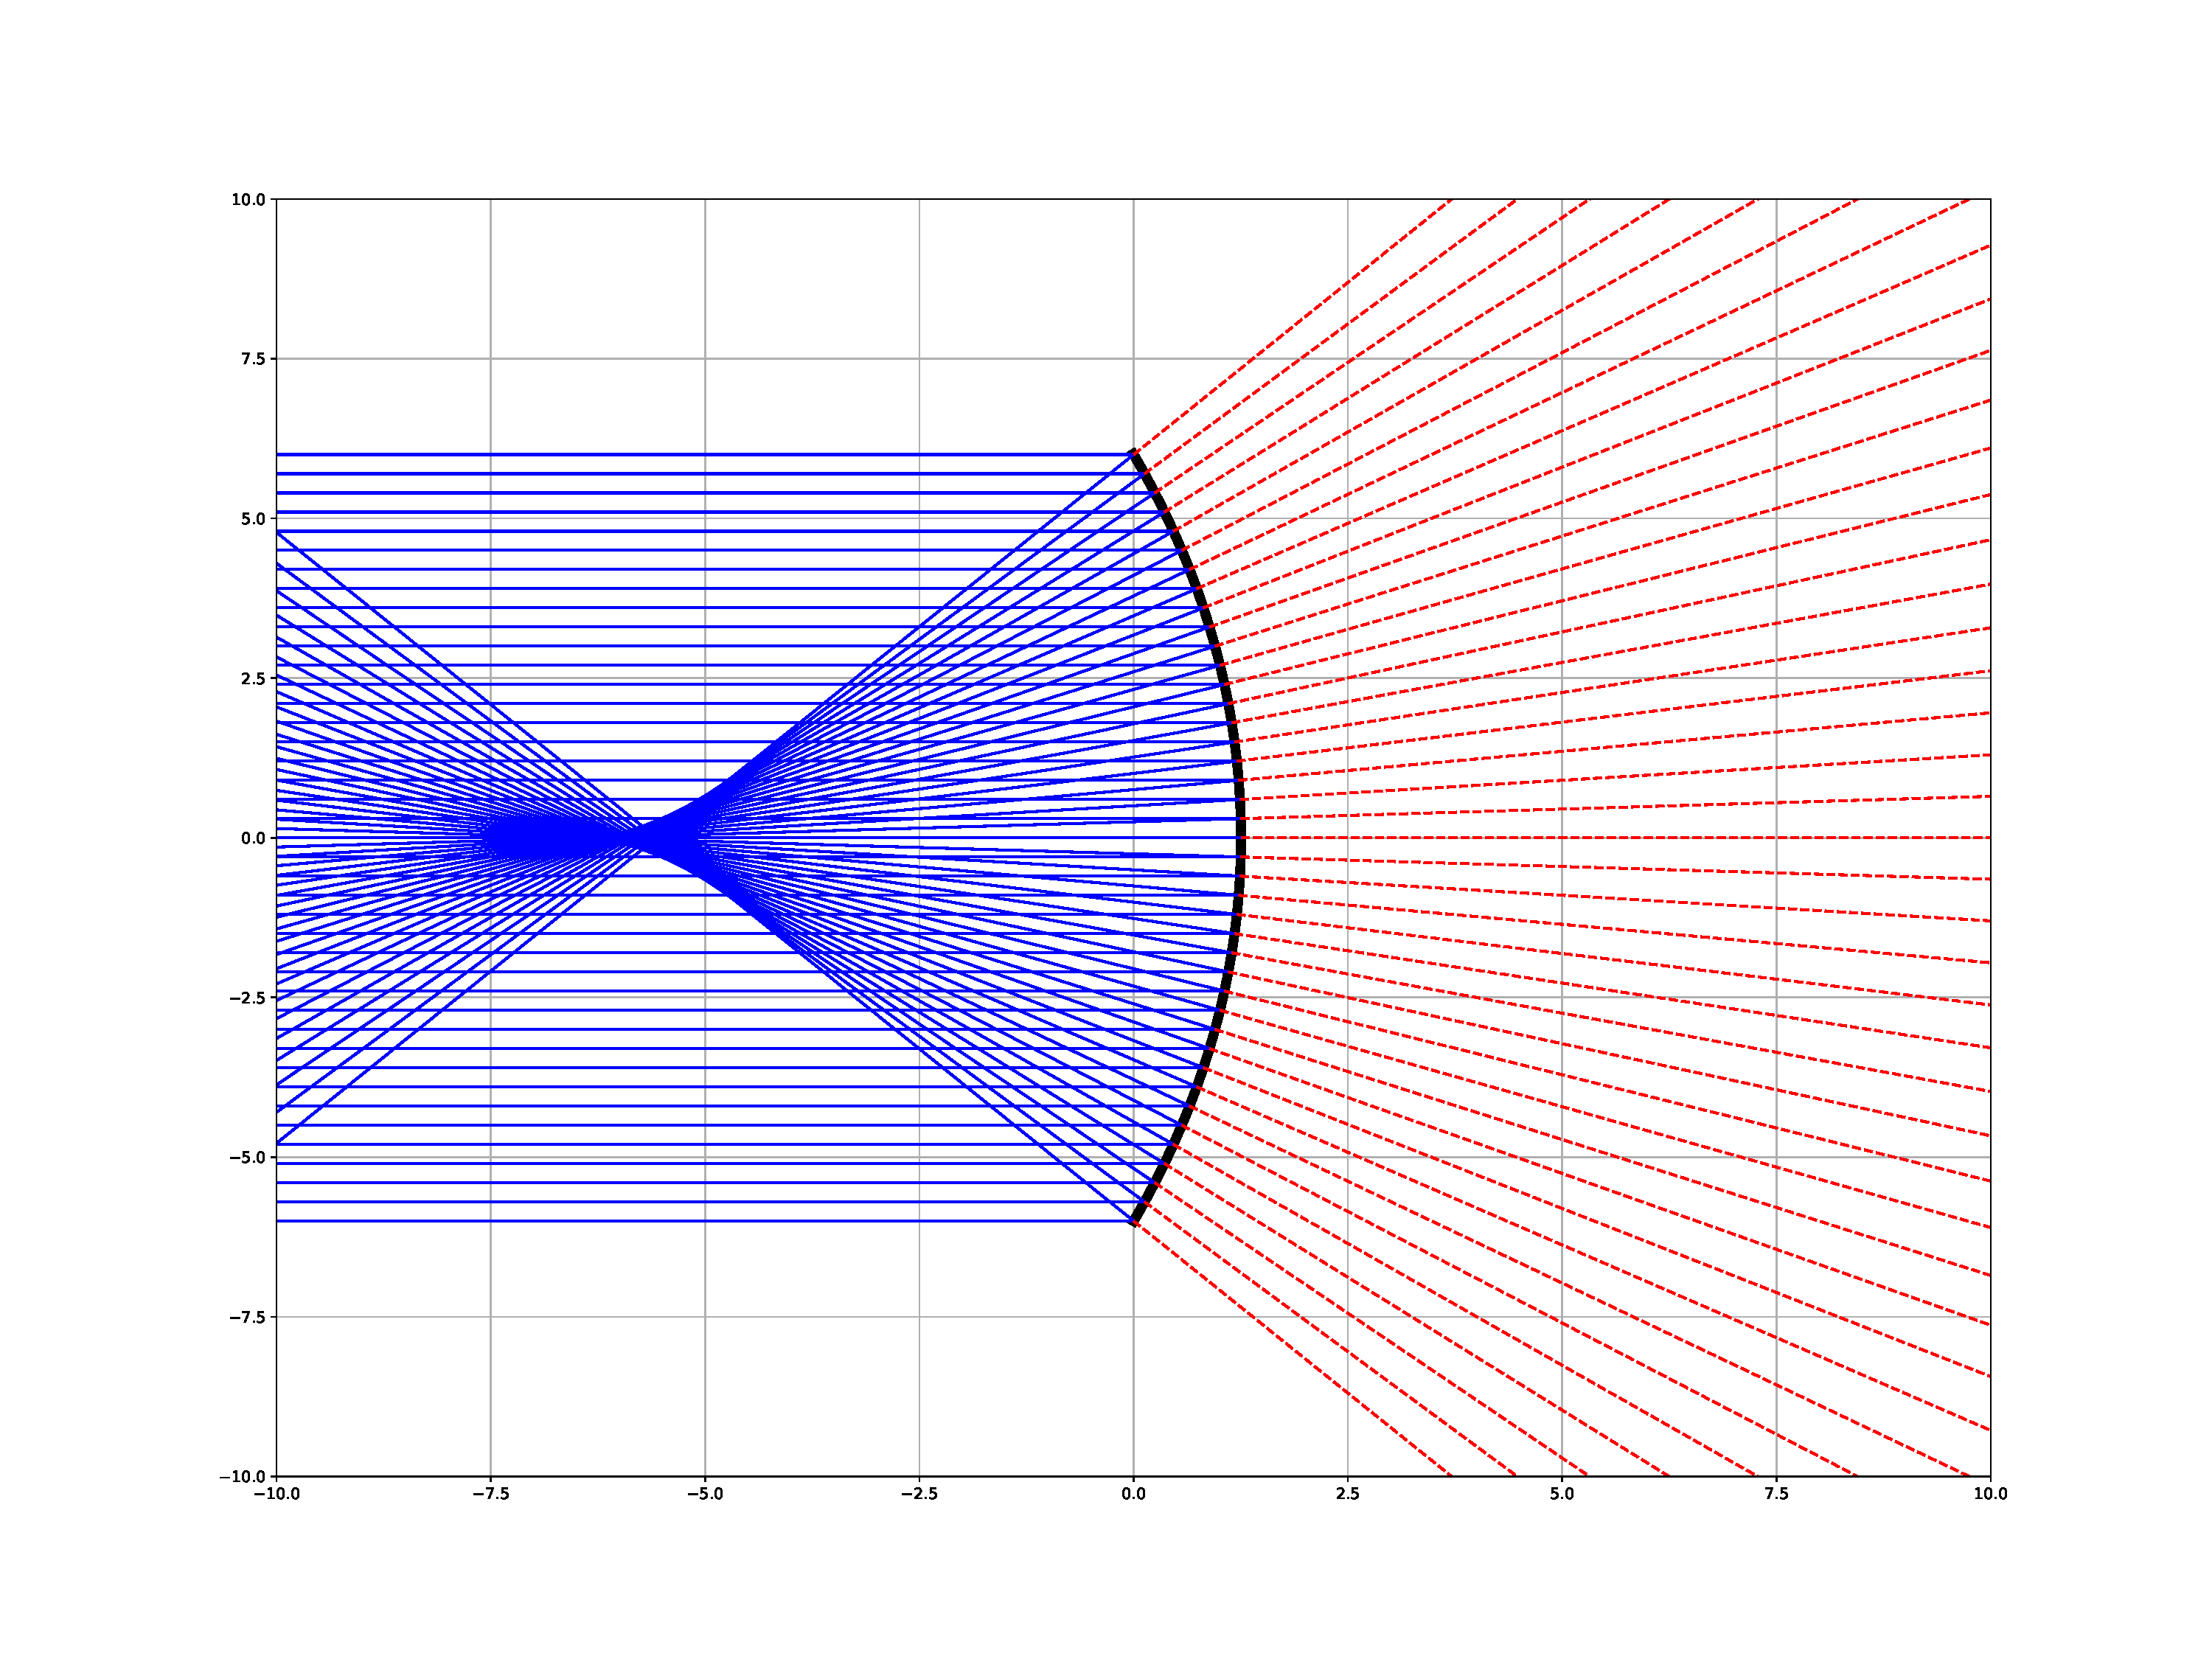
\includegraphics[width=\linewidth]{Figures/Figures_miroirs/conc_pastig.pdf}
		\caption{Miroir concave avec faisceau large}
		\label{fig:conc_pastig} 
    \end{subfigure}
    ~
    \begin{subfigure}[t]{0.45\linewidth}
    	\centering
		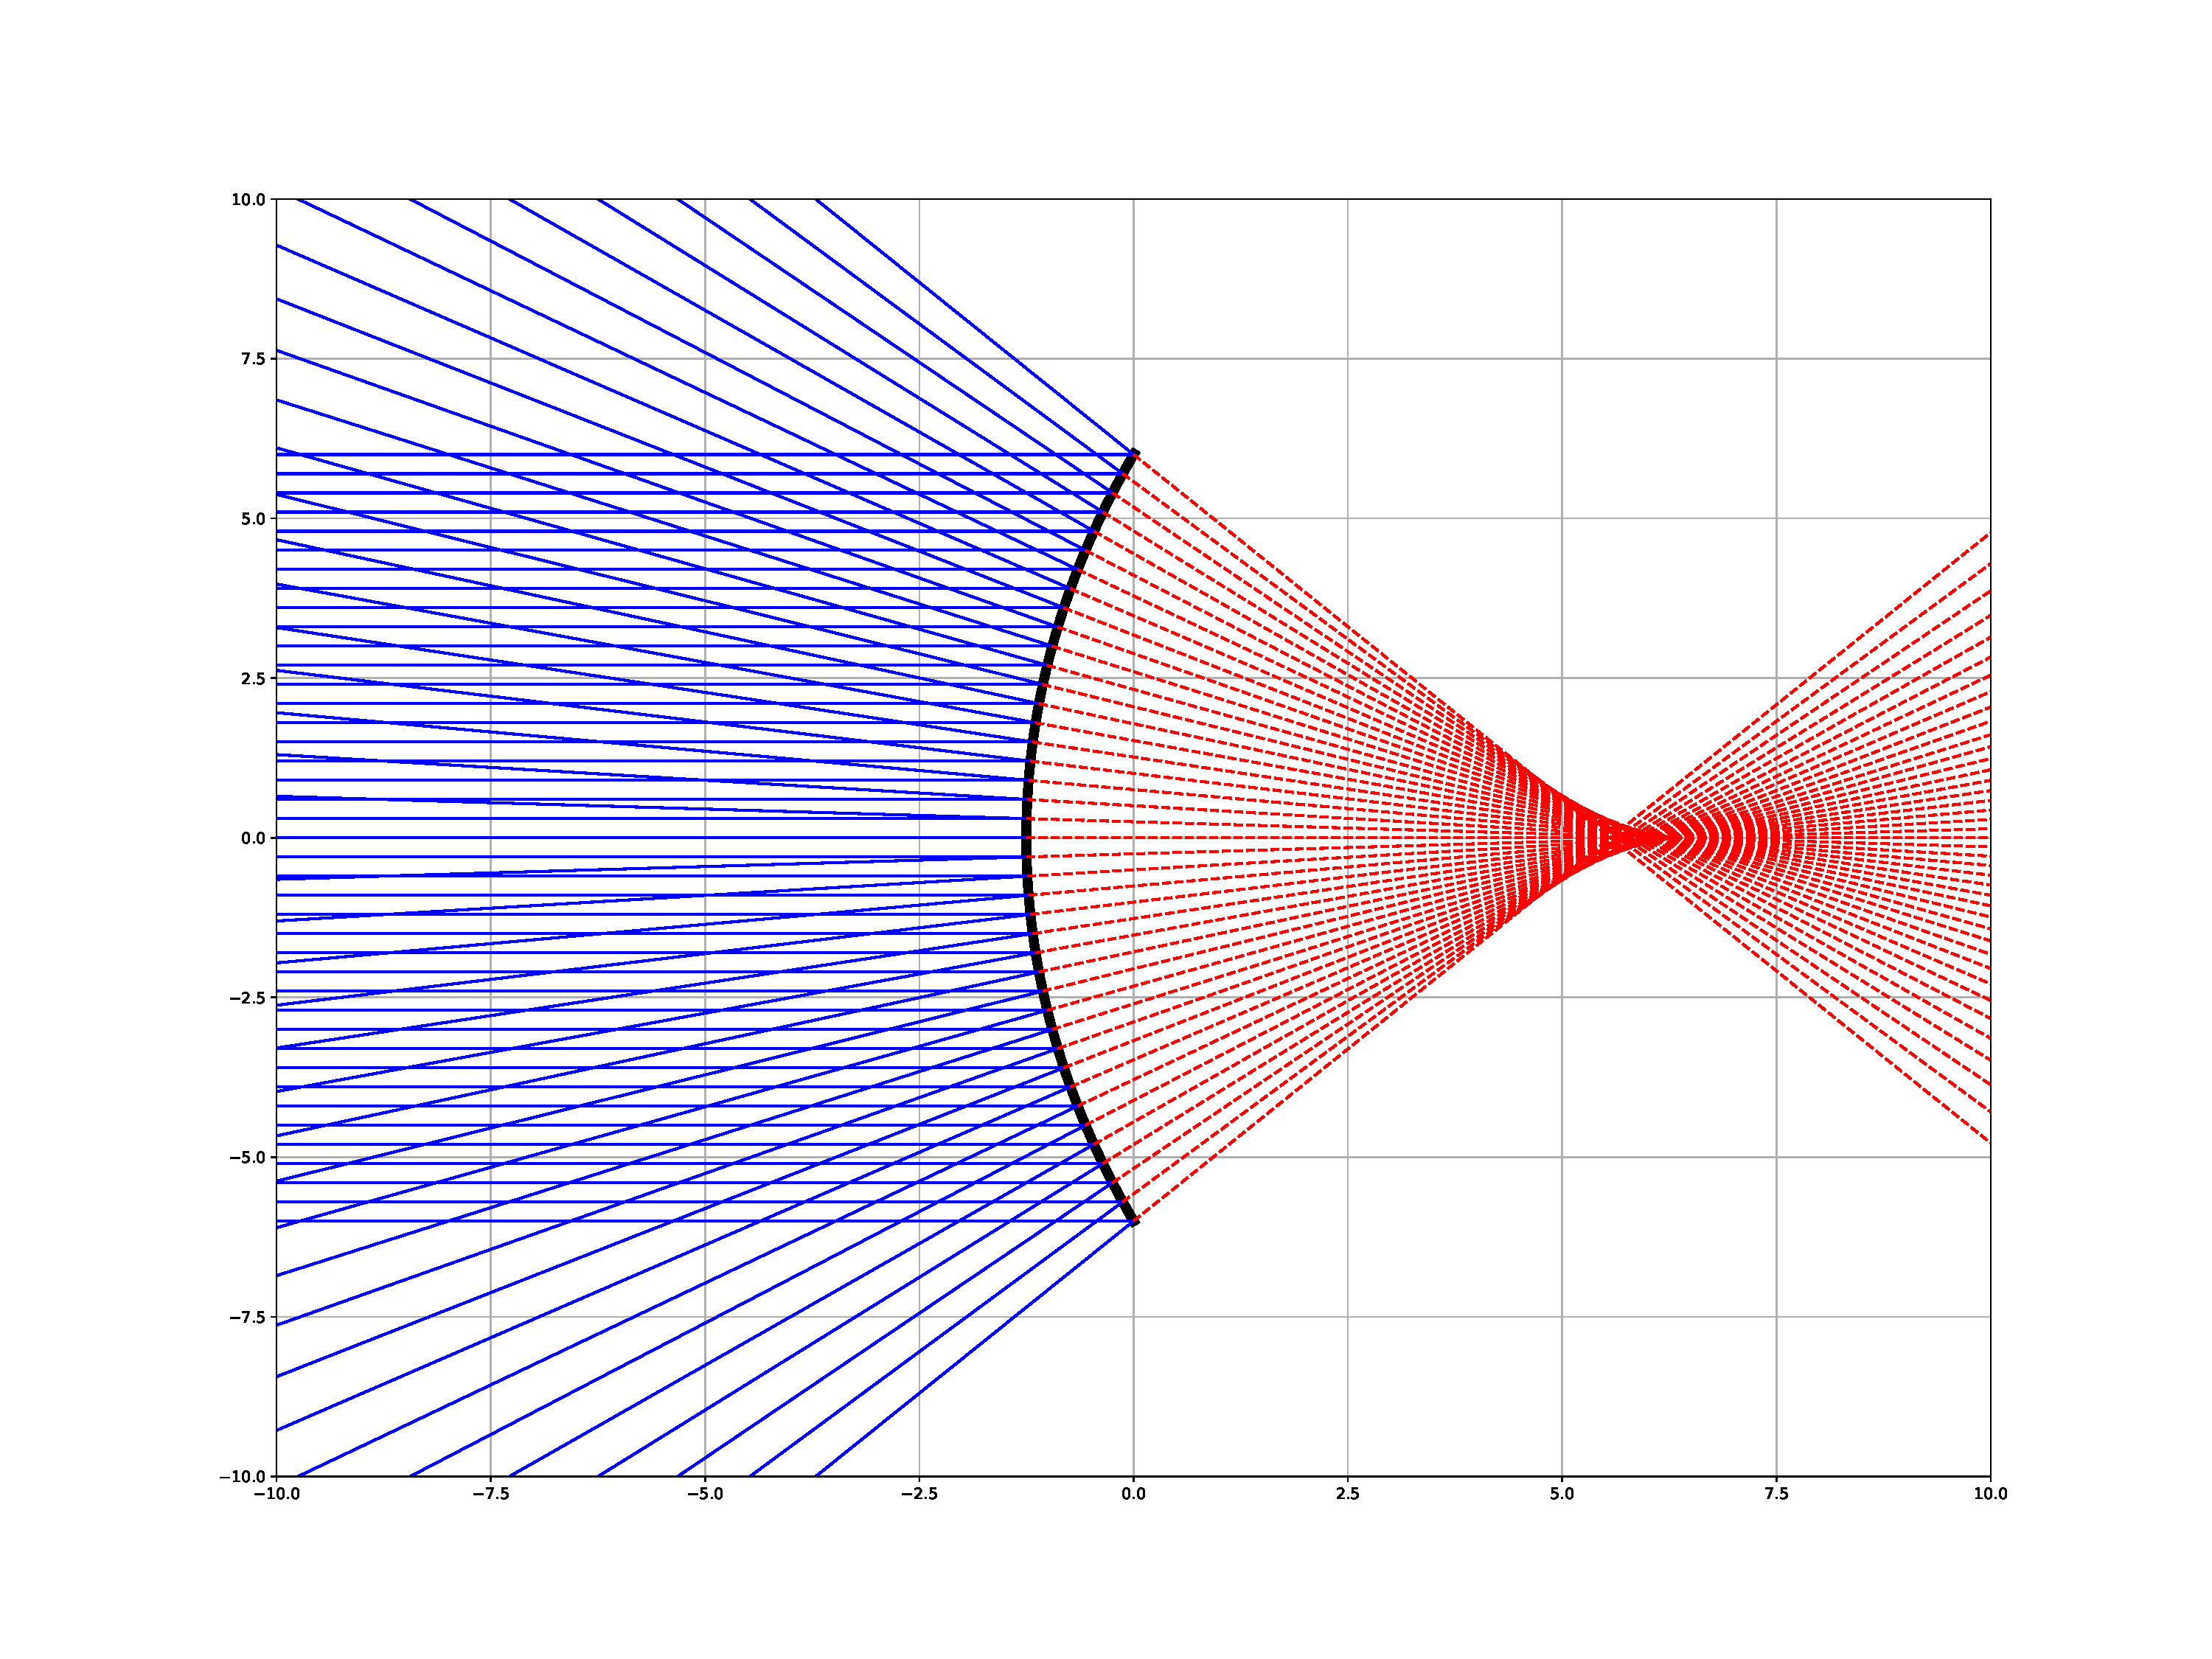
\includegraphics[width=\linewidth]{Figures/Figures_miroirs/conv_pastig.pdf}
		\caption{Miroir convexe avec faisceau large}
		\label{fig:conv_pastig} 
    \end{subfigure}
\hfill
    \begin{subfigure}[t]{0.45\linewidth}
    	\centering
		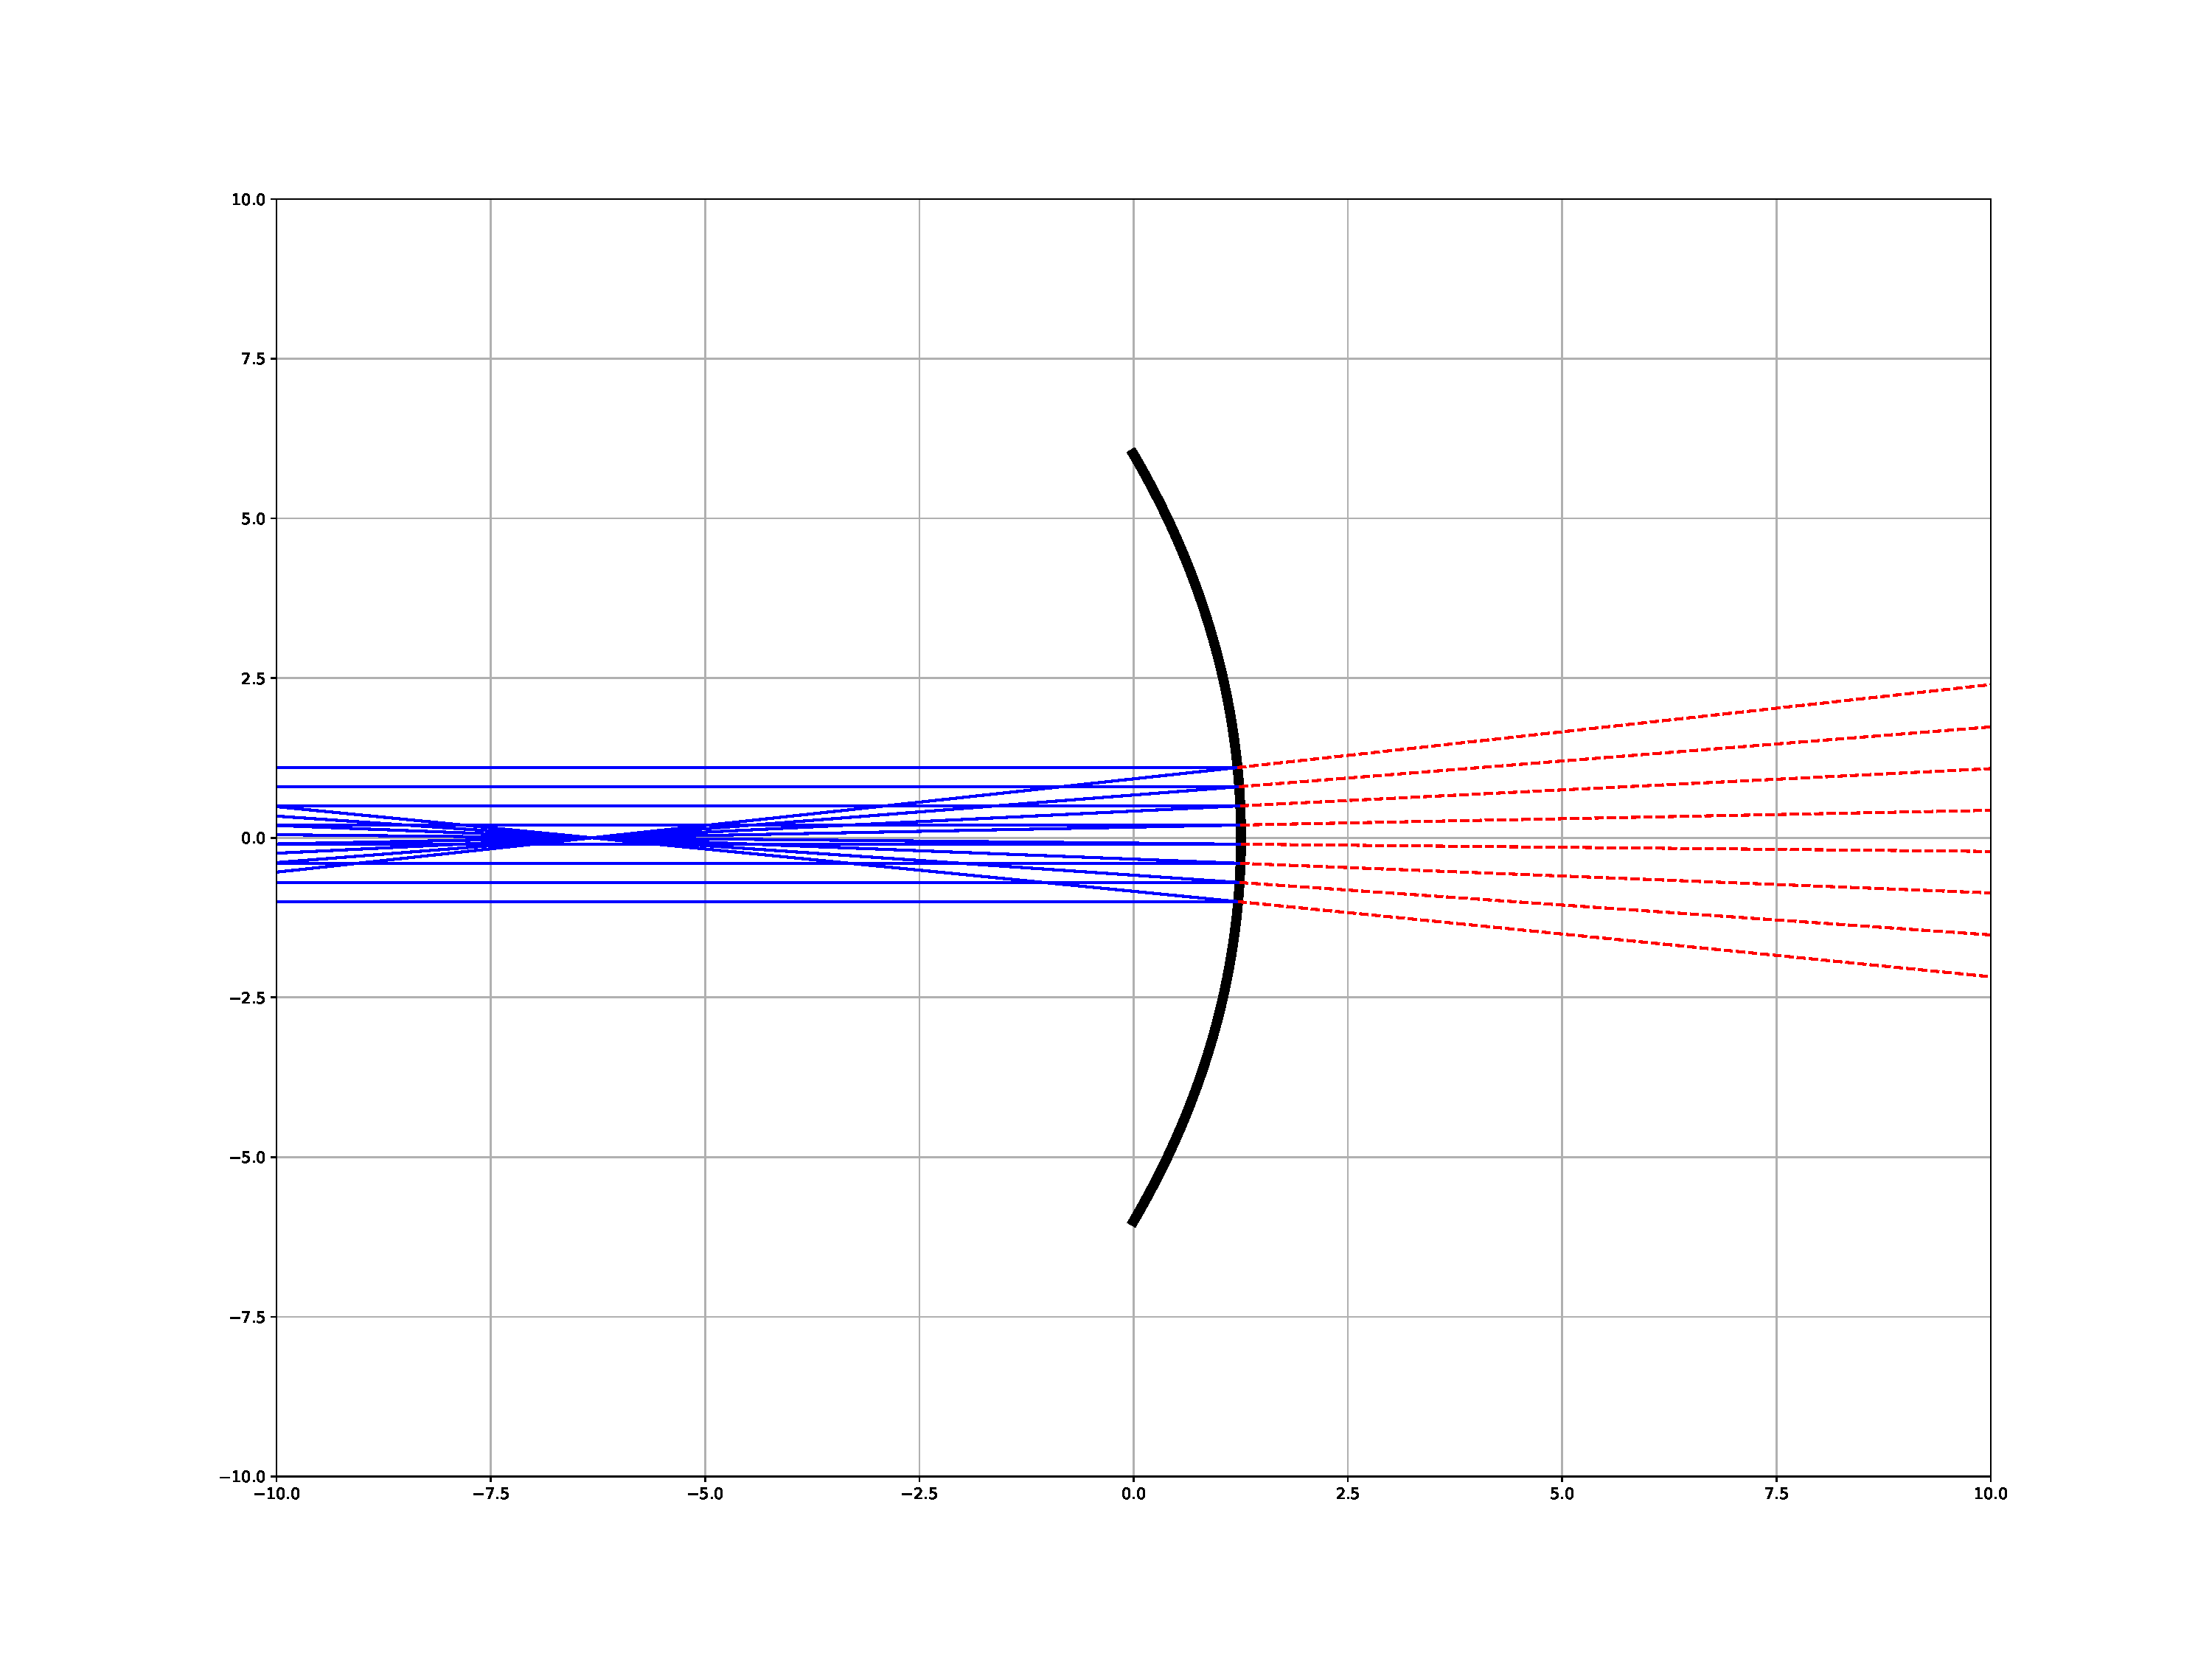
\includegraphics[width=\linewidth]{Figures/Figures_miroirs/conc_stig.pdf}
		\caption{Miroir concave avec faisceau fin}
		\label{fig:conc_stig}
    \end{subfigure}
    ~
    \begin{subfigure}[t]{0.45\linewidth}
    	\centering
		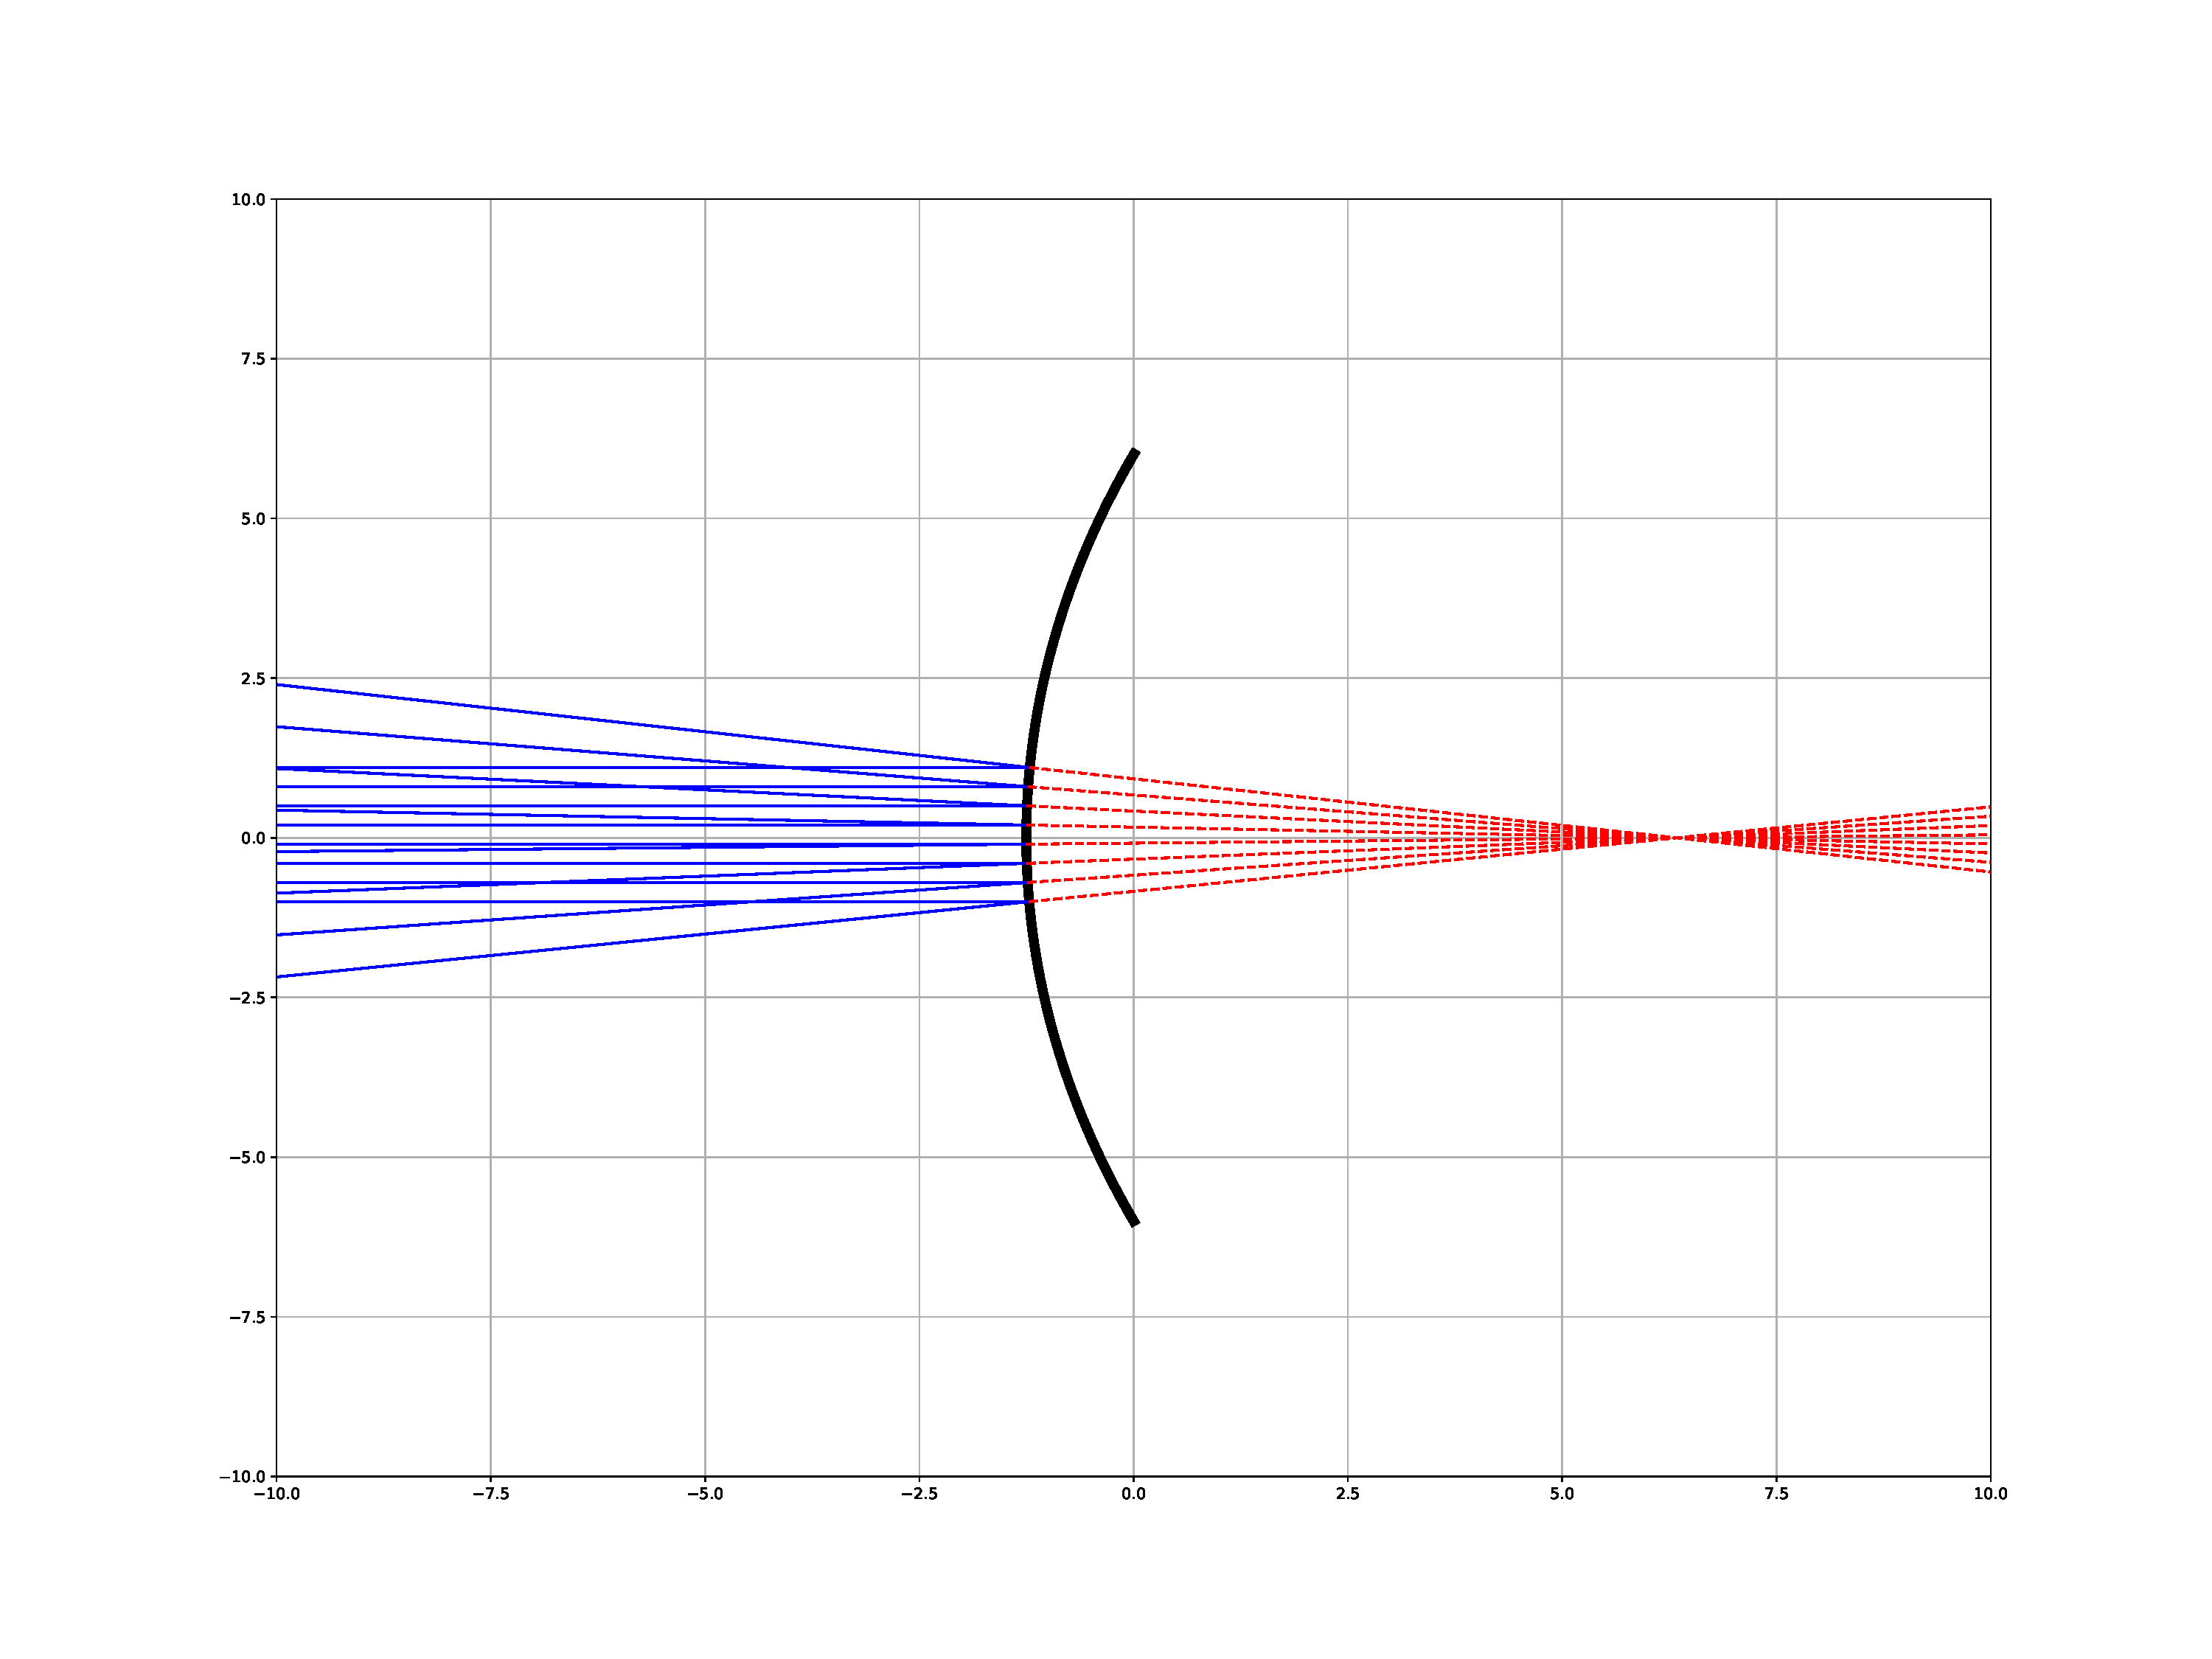
\includegraphics[width=\linewidth]{Figures/Figures_miroirs/conv_stig.pdf}
		\caption{Miroir convexe avec faisceau fin}
		\label{fig:conv_stig}
    \end{subfigure}

    \caption{Miroirs sphériques concave et convexe dans les cas où le faisceau lumineux est large ou fin}
    \label{fig:miroirs}
\end{figure}

Il apparaît ici que les dioptres en question (ici des miroirs) peuvent être considérés comme des systèmes stigmatiques approchés quand les rayons lumineux sont situés vers le centre du miroir sphérique. Pour la hauteur du faisceau, le rayon de la lentille est très élevé (on peut même dire que $r \longrightarrow \infty$) donc le miroir sphérique se comporte comme un miroir plan, qui est un système stigmatique. Or, d'après le cours d'optique géométrique de L1 SPI, si la taille du faisceau est négligeable devant le rayon du dioptre, alors le système est dit "dans les conditions de Gauss". On peut donc en conclure à l'aide de ces illustrations qu'un système optique peut être considéré comme stigmatique dans les conditions de Gauss, c'est-à-dire quand le faisceau est localisé au centre du système optique et pas sur les bords.


\subsubsection{Lentilles sphériques biconcaves et biconvexes}
La seconde classe à développer dans ce projet est la classe \verb|Lentille| comprenant des méthodes afin de tracer les différents types de lentilles: \verb|biconcave| et \verb|biconvexe| ainsi qu'une méthode \verb|rayon| qui calcule les trajectoires des rayons lumineux pour chaque cas. Les cas permettant de mettre en évidence le stigmatisme sont réutilisés ici, donc il y a une figure pour chacun des 2 dioptres pour chaque cas: pour un faisceau large et un faisceau fin. Ces 4 cas sont présentés en figure \ref{fig:lentilles}. 

\begin{figure}[H]
    \centering
    \begin{subfigure}[t]{0.45\linewidth}
    	\centering
		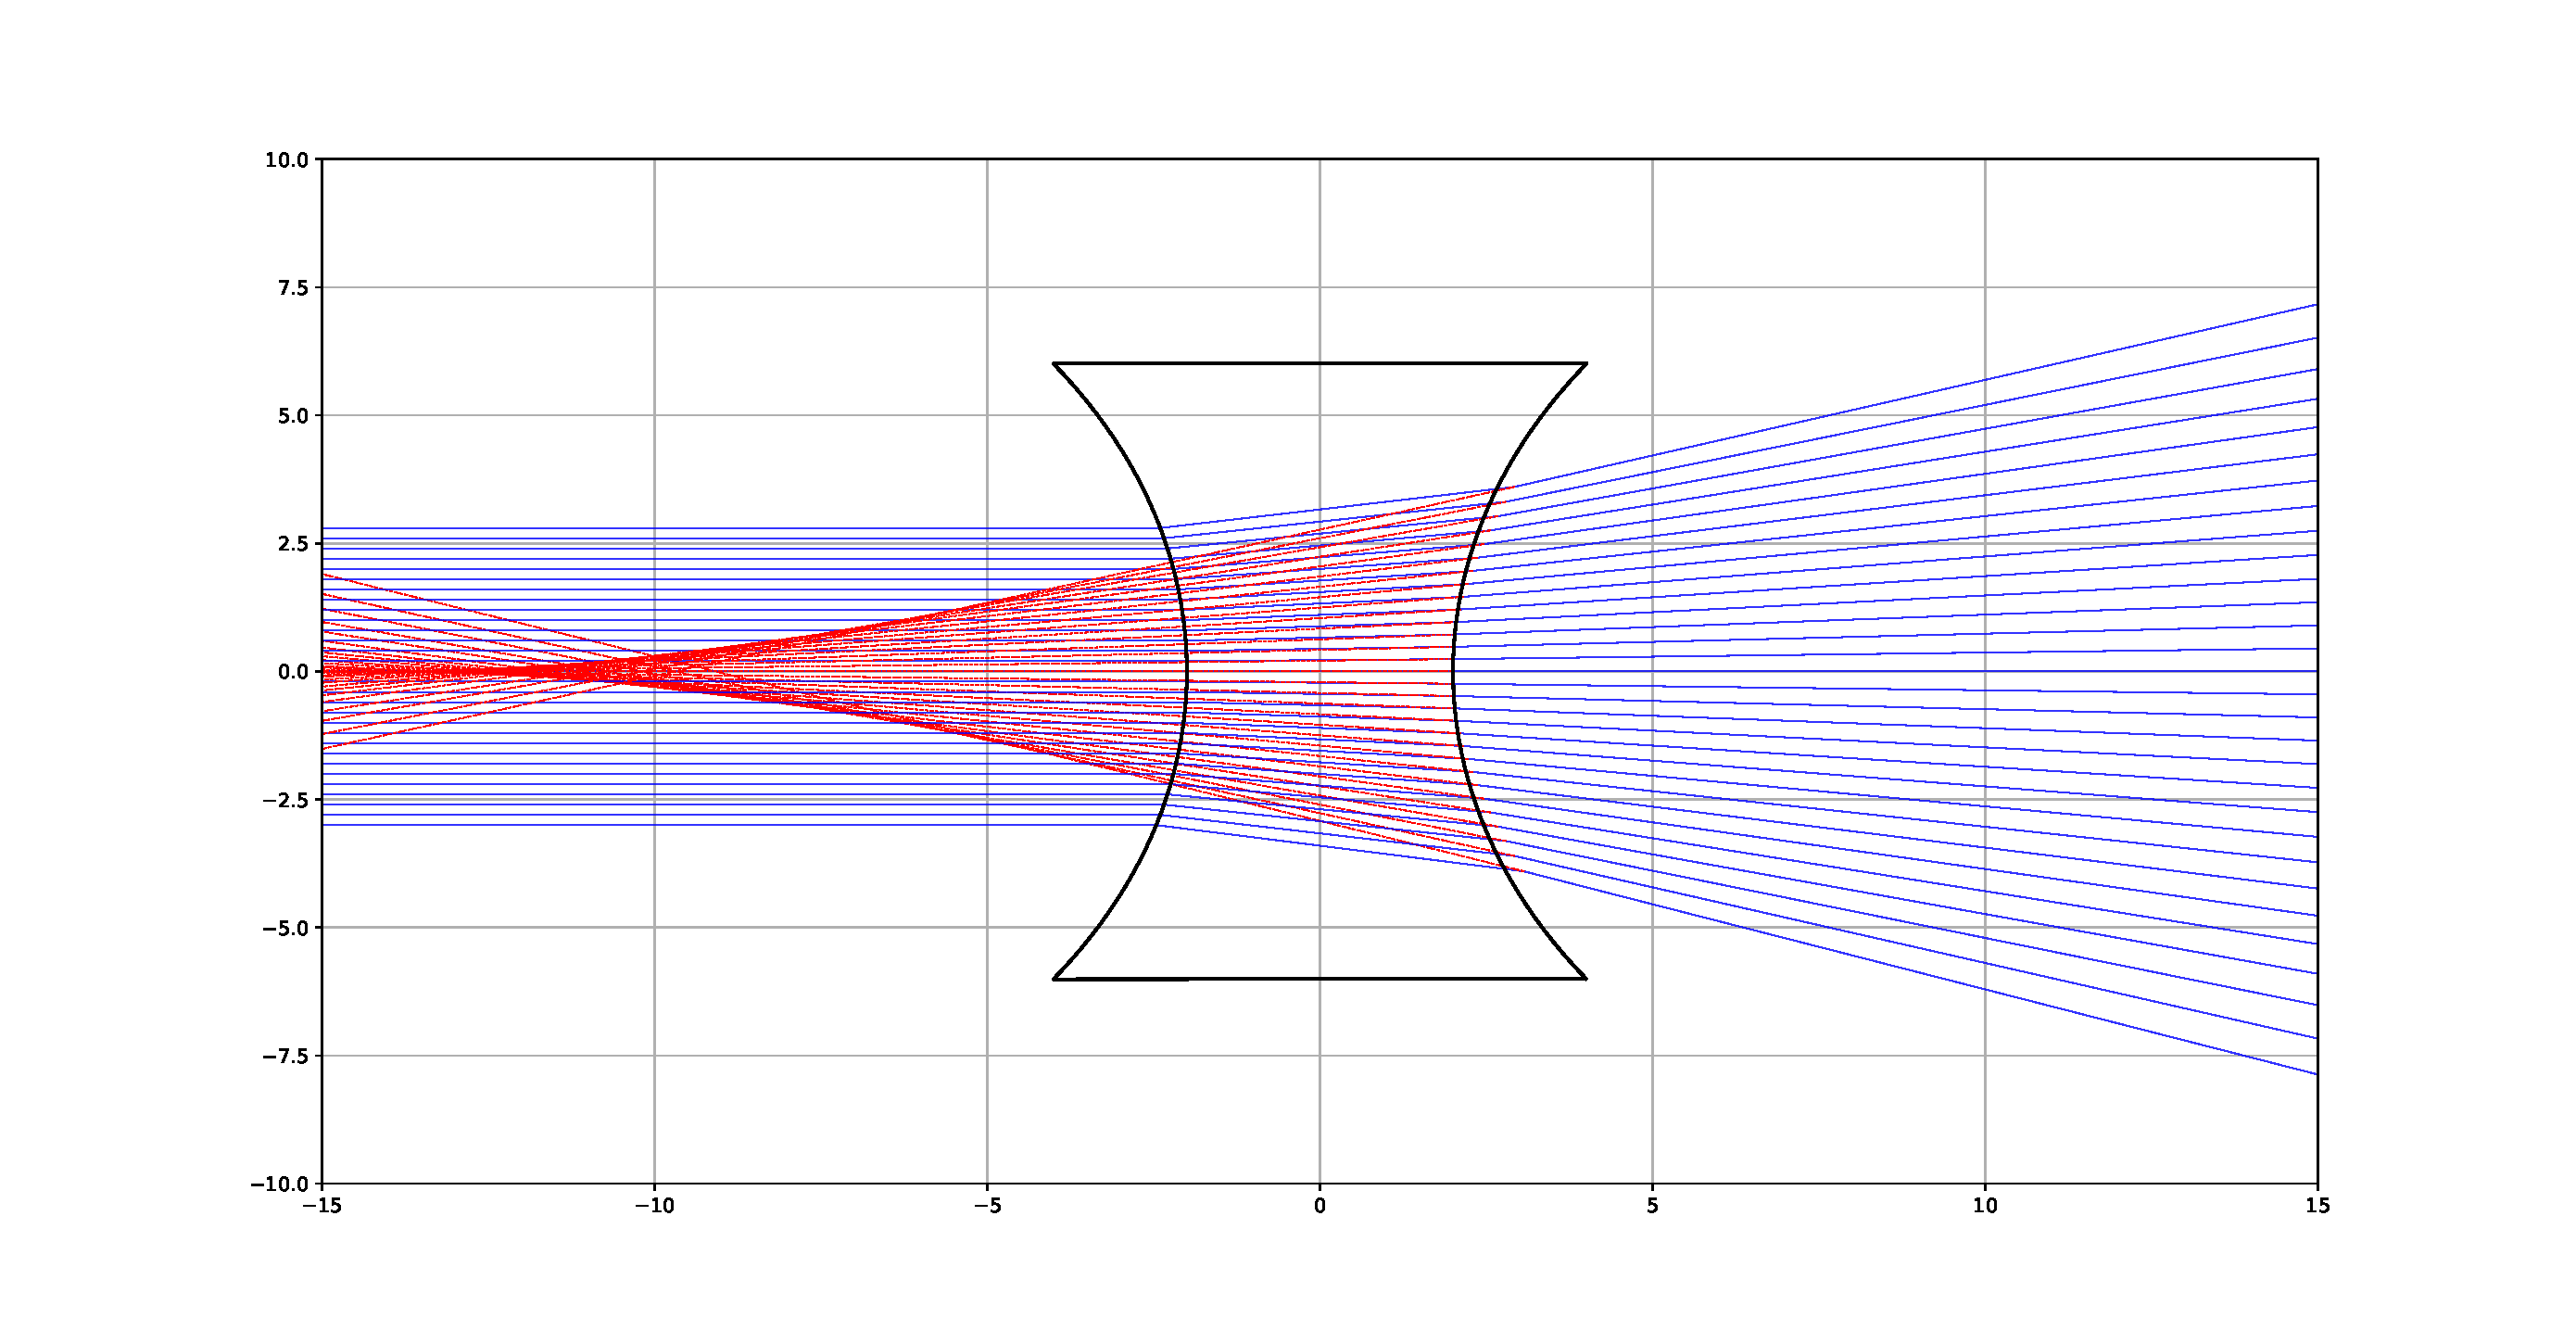
\includegraphics[width=\linewidth]{Figures/Figures_lentilles/biconcave_pastig.pdf}
		\caption{Lentille biconcave avec faisceau large}
		\label{fig:conc_pastig} 
    \end{subfigure}
    ~
    \begin{subfigure}[t]{0.45\linewidth}
    	\centering
		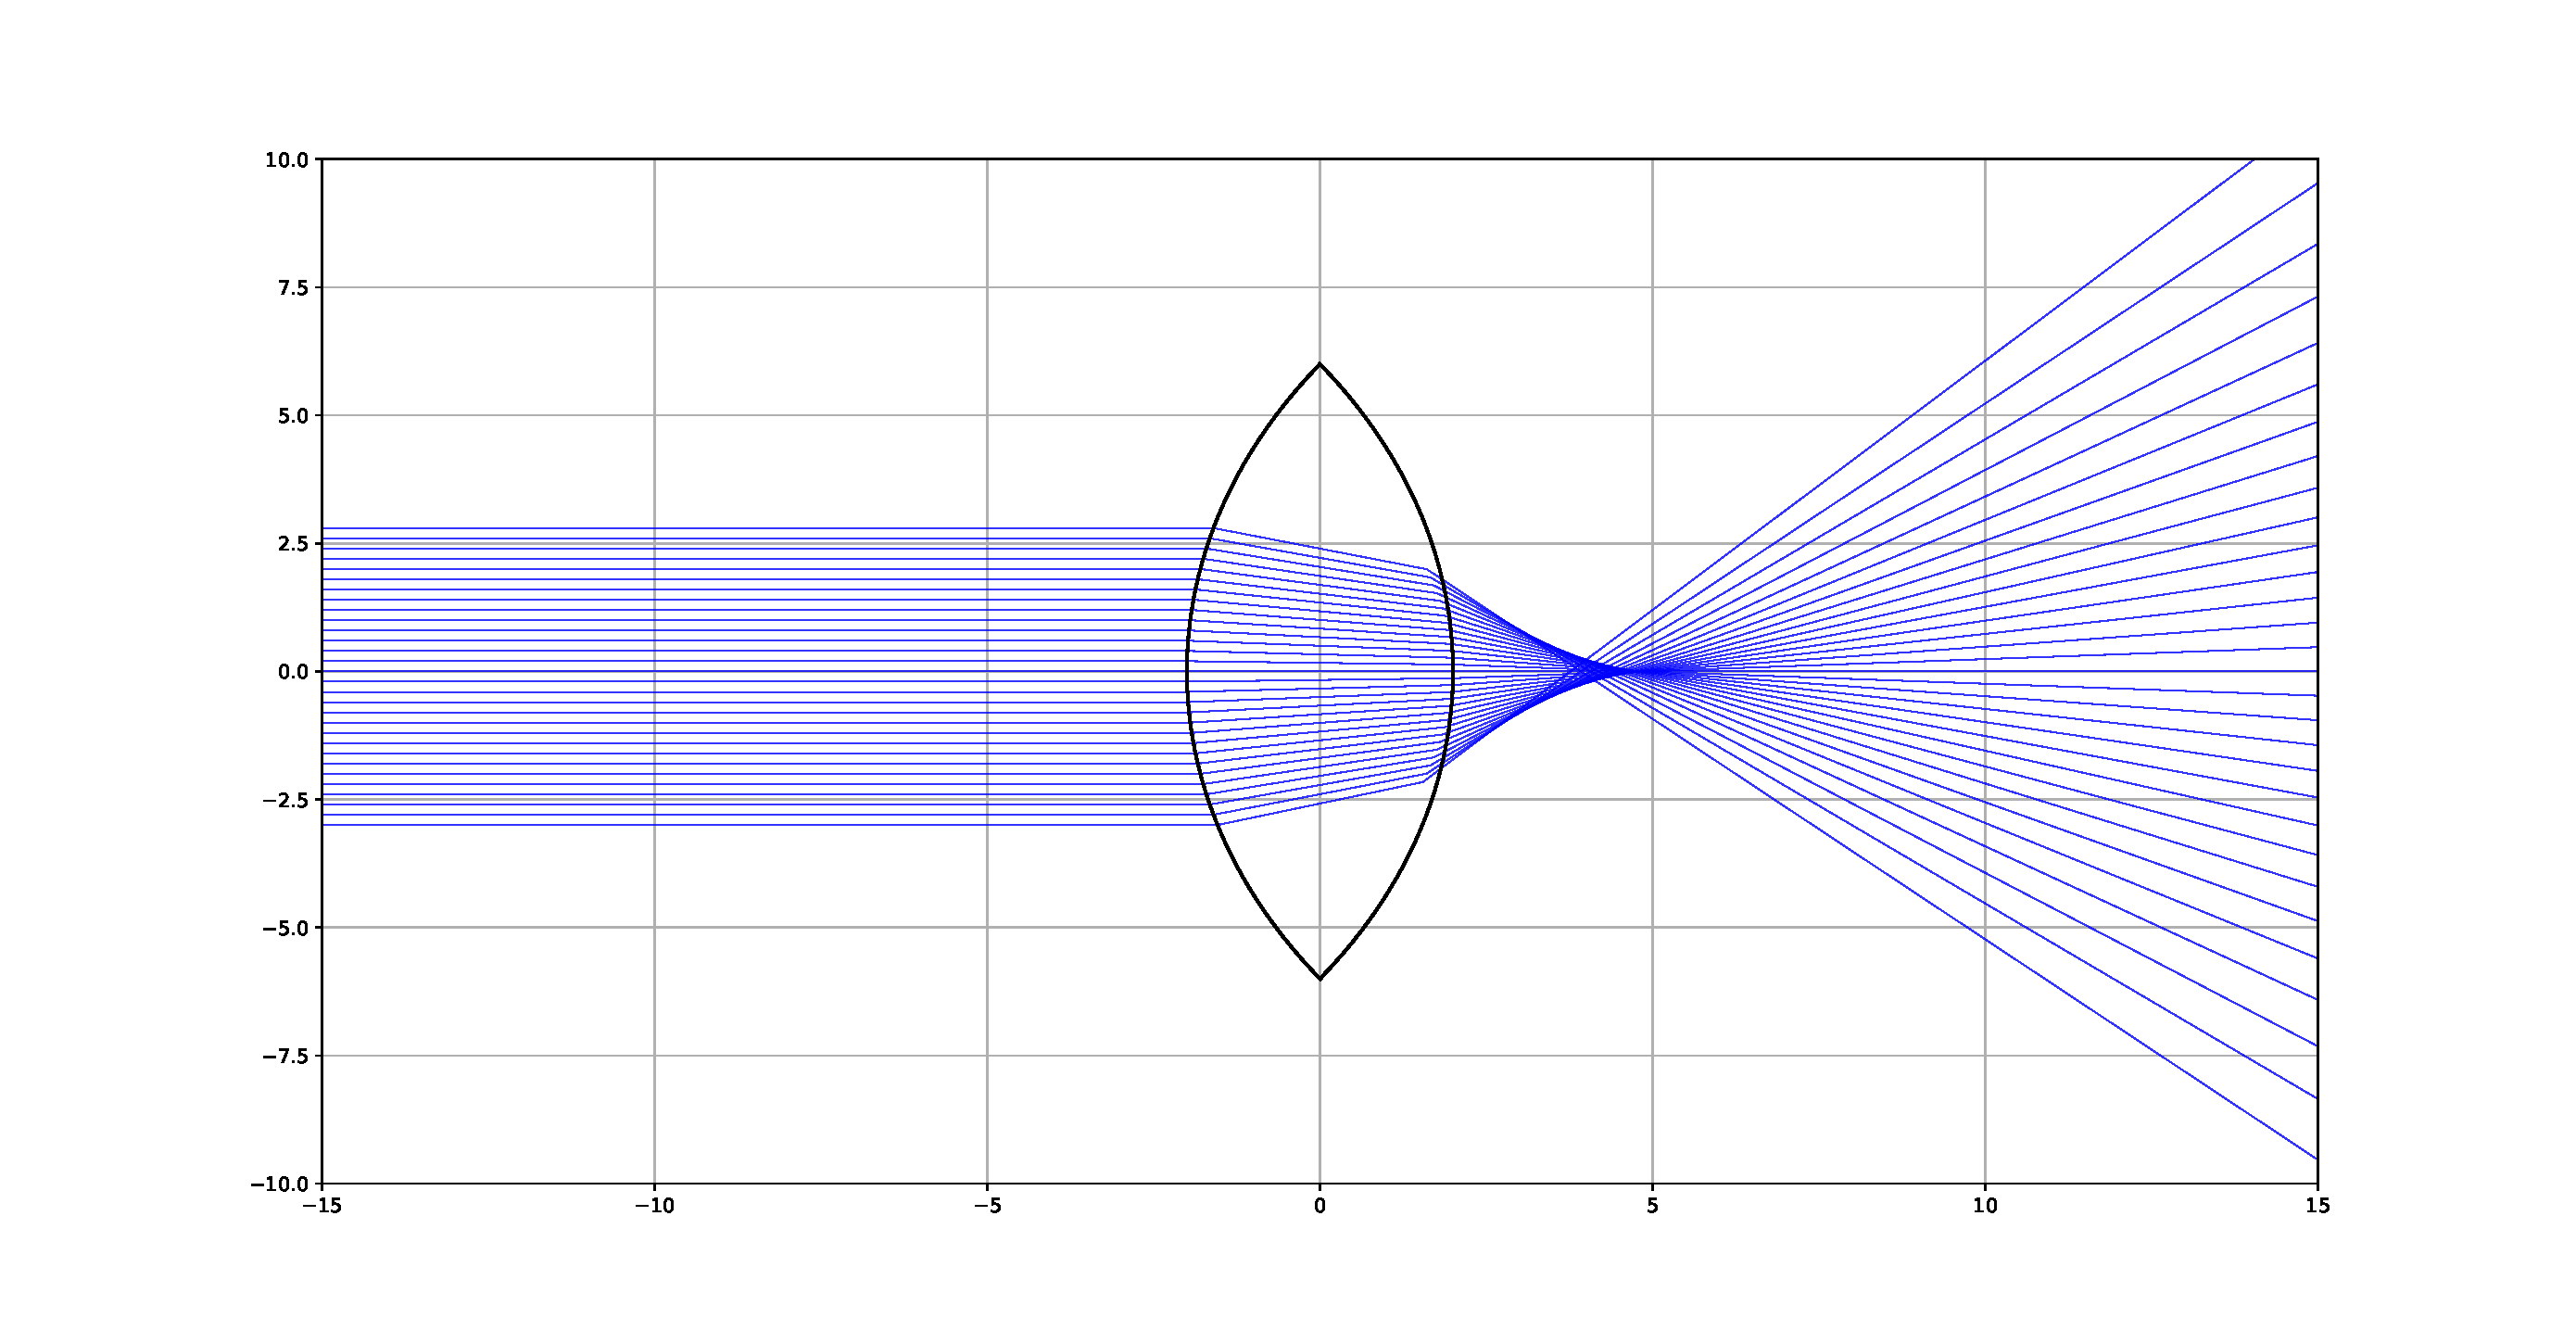
\includegraphics[width=\linewidth]{Figures/Figures_lentilles/biconvexe_pastig.pdf}
		\caption{Lentille biconvexe avec faisceau large}
		\label{fig:conv_pastig} 
    \end{subfigure}
\hfill
    \begin{subfigure}[t]{0.45\linewidth}
    	\centering
		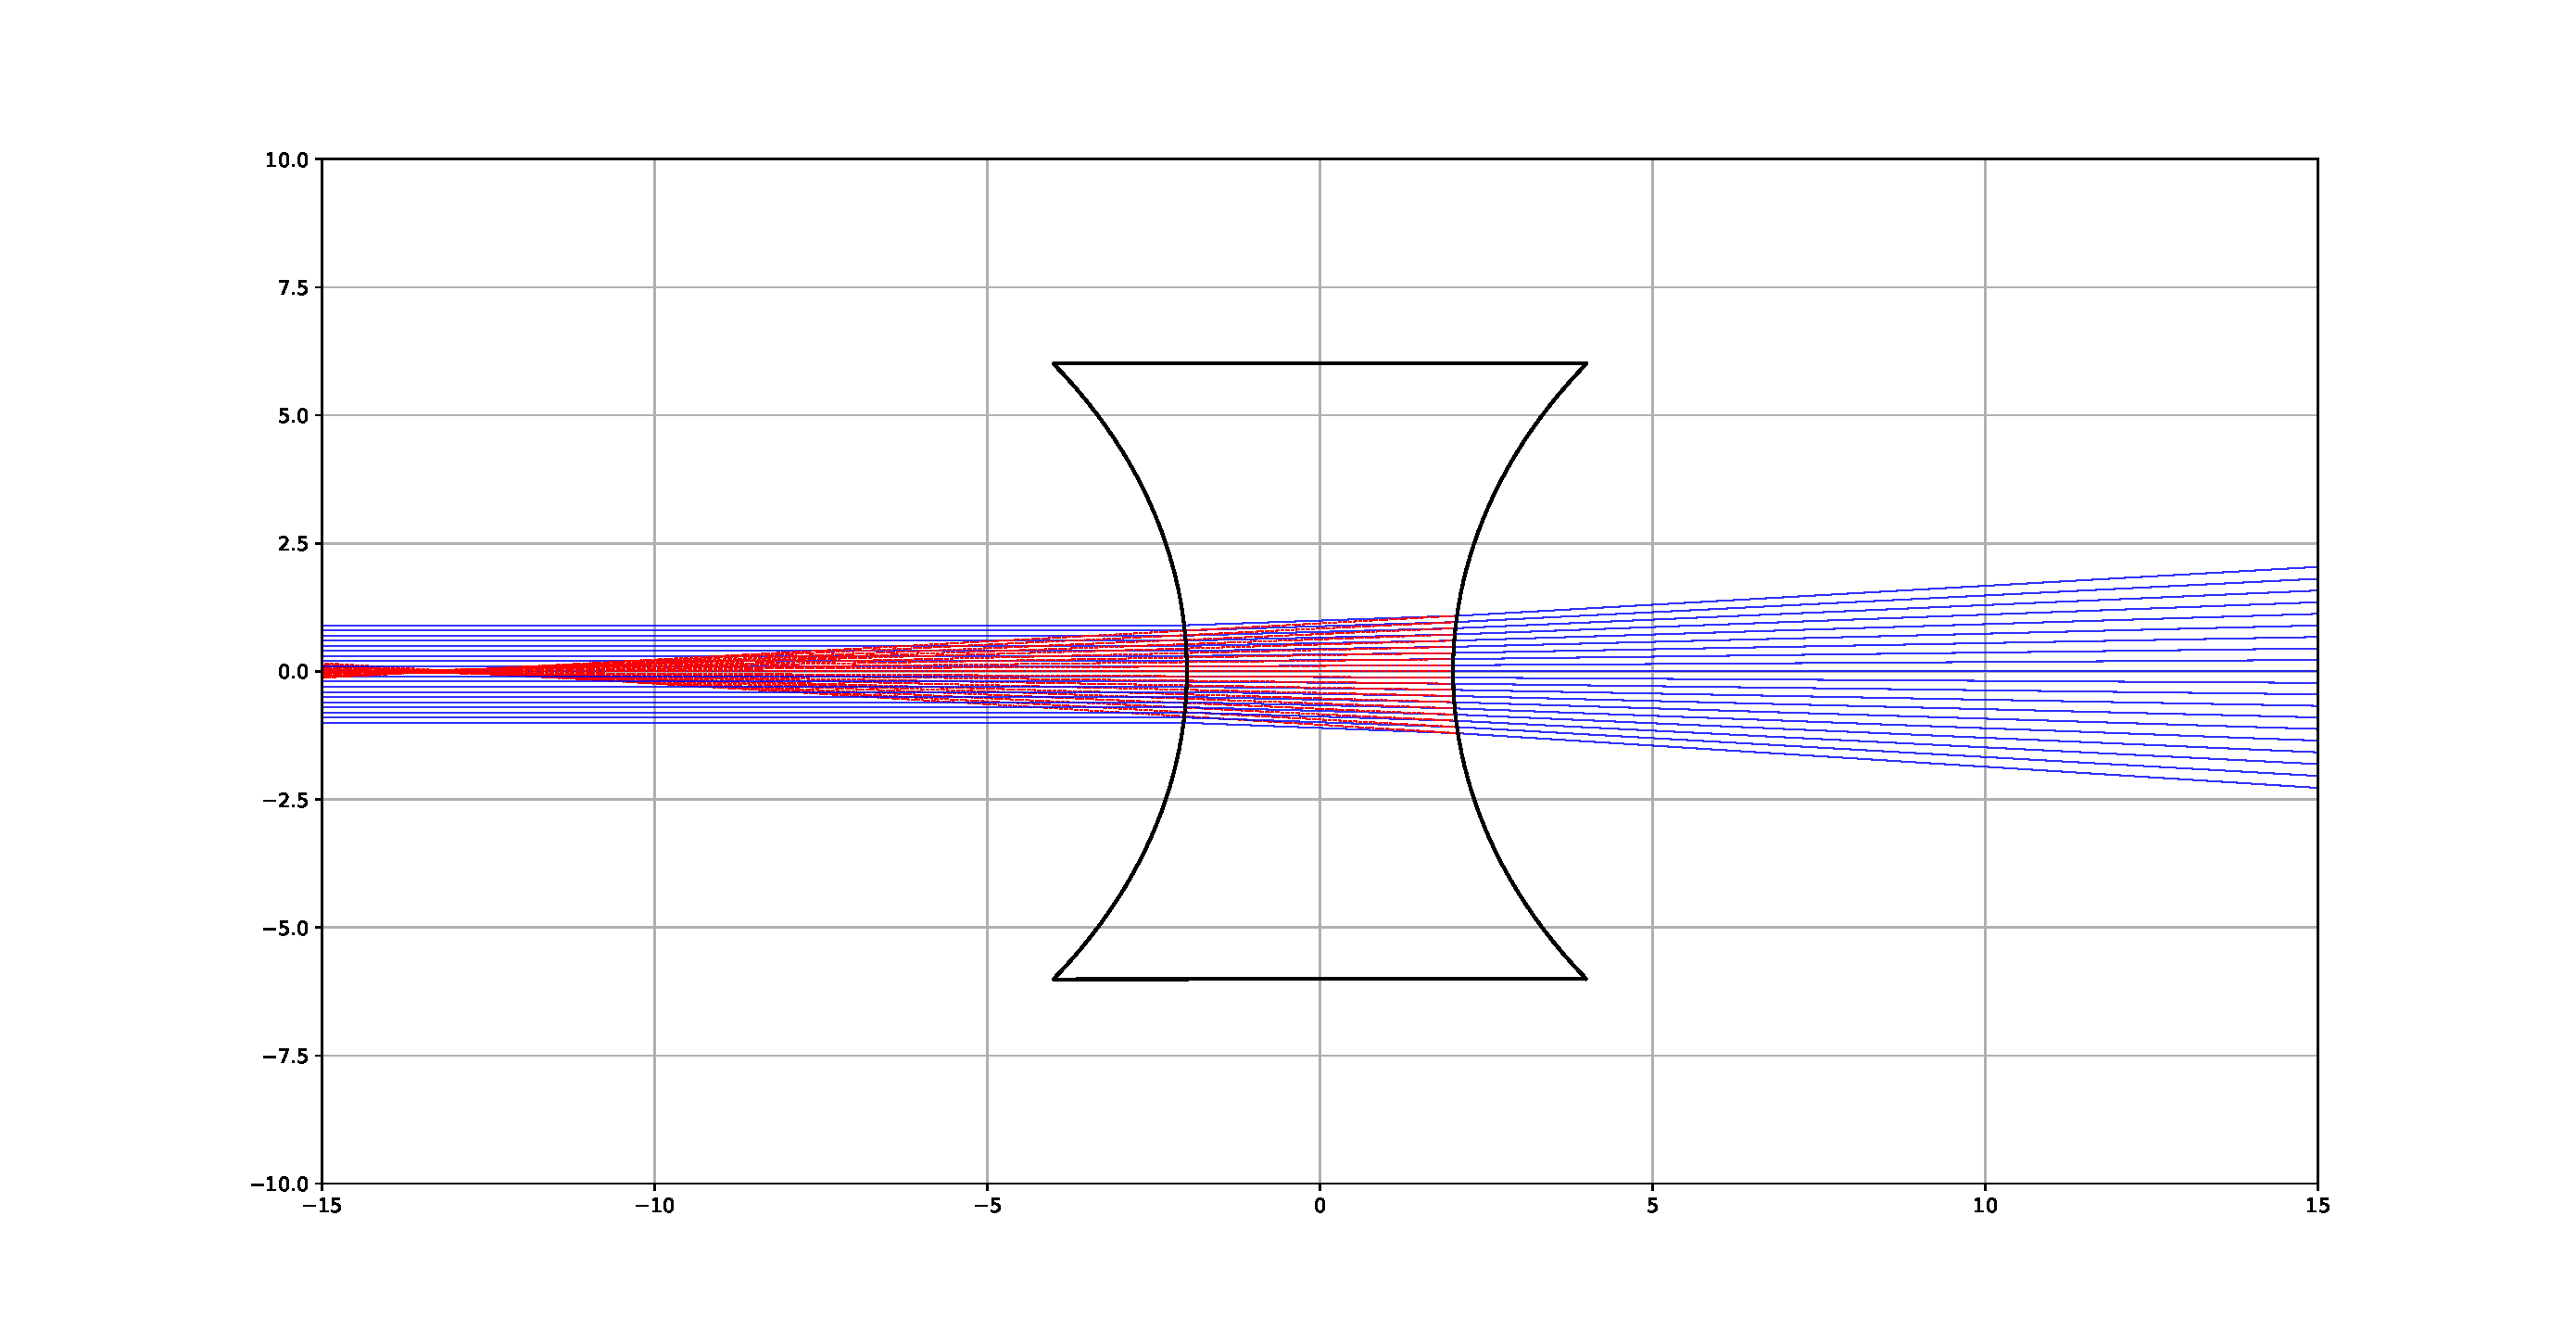
\includegraphics[width=\linewidth]{Figures/Figures_lentilles/biconcave_stig.pdf}
		\caption{Lentille biconcave avec faisceau fin}
		\label{fig:conc_stig}
    \end{subfigure}
    ~
    \begin{subfigure}[t]{0.45\linewidth}
    	\centering
		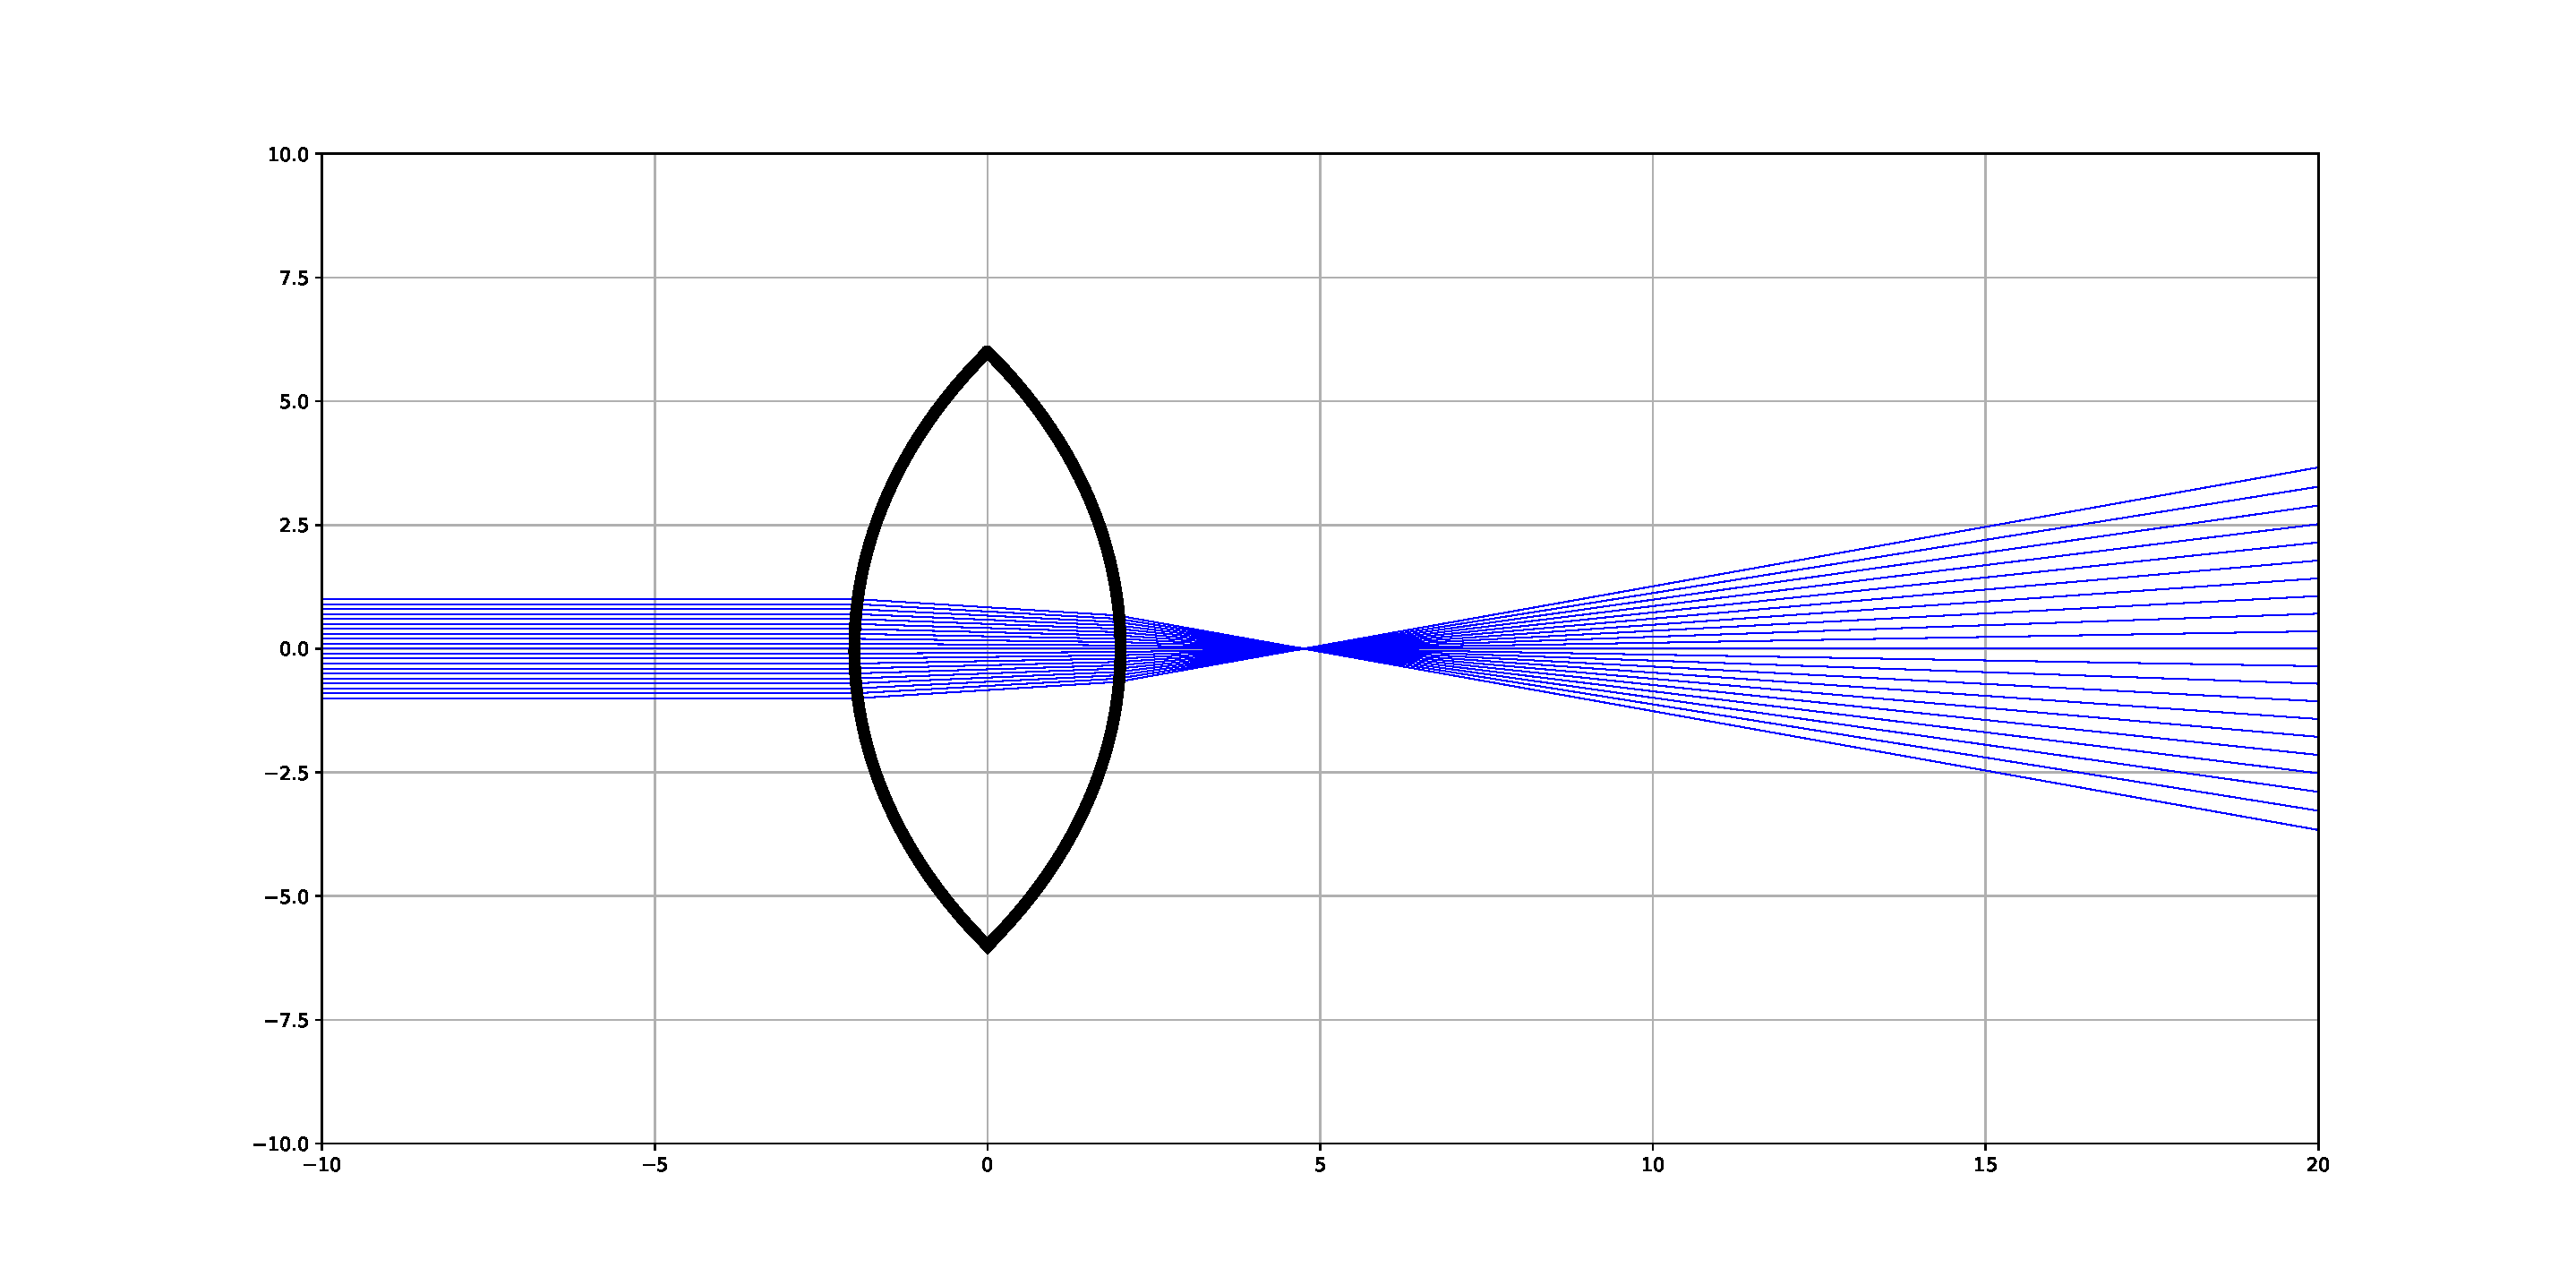
\includegraphics[width=\linewidth]{Figures/Figures_lentilles/biconvexe_stig.pdf}
		\caption{Lentille biconvexe avec faisceau fin}
		\label{fig:conv_stig}
    \end{subfigure}

    \caption{Lentilles sphériques biconcave et biconvexe dans les cas où le faisceau lumineux est large ou fin}
    \label{fig:lentilles}
\end{figure}

Pour obtenir ces figures, les mêmes relations géométrique que celles définies pour la partie des miroirs sphériques sont réutilisées, avec quelques variations. Ainsi, on peut réutiliser le code créé pour les miroirs pour calculer les coordonnées des points pour ces 2 types de lentilles. Les coordonnées des points et angles à définir sont:
\begin{itemize}
	\item la coordonnée en $x$ du rayon, où celui-ci est transmis, \verb|x_r1|
	\item l'angle de réflexion sur le premier dioptre, \verb|i_2|
	\item les coordonnées $x$ et $y$ du rayon quand il atteint le deuxième dioptre, \verb|x_r2| et \verb|y_r1|
	\item l'angle de réflexion sur le deuxième dioptre, \verb|i_2|
	\item la hauteur du rayon à la limite \verb|y_r2|
\end{itemize}

Tous les calculs de ces points sont réalisés en réutilisant les formules utilisées pour les miroirs avec quelques changements. Cette méthode est certes rapide, mais peu précise et rend le code permettant de tracer ces figures difficile à lire et à exploiter. De plus, l'adaptation des formules demande de changer les signes des formules, engendrant quelques bugs tel que celui représenté en figure \ref{fig:bug_lentille}.

\begin{figure}[H]
	\centering
	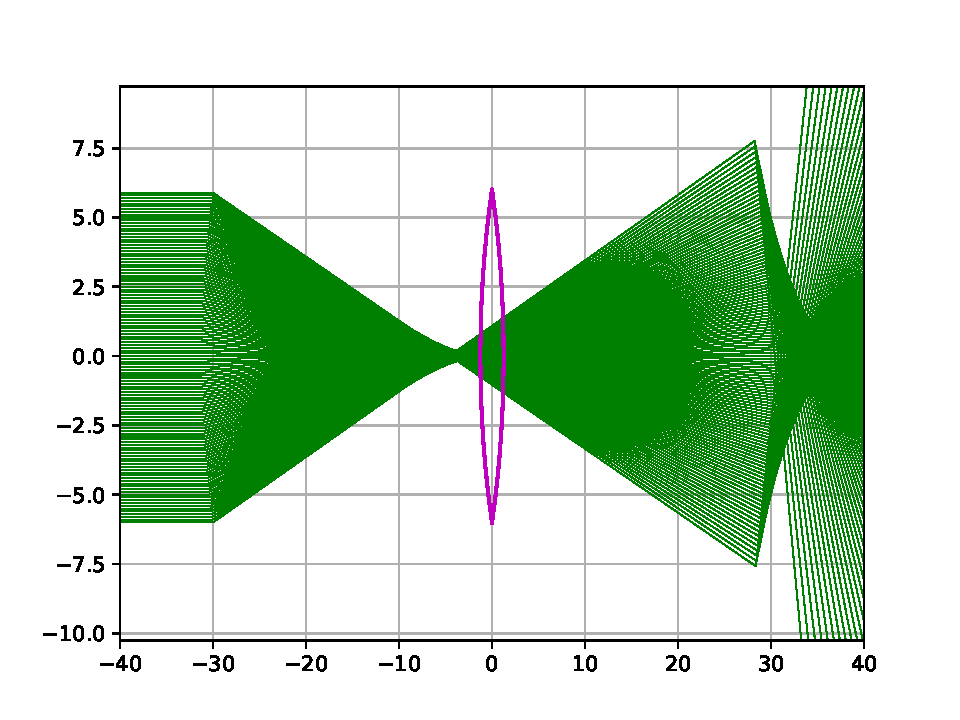
\includegraphics[scale=0.6]{Figures/bug_lentille.pdf}
	\caption{Problème rencontré lors du calcul des différents points nécessaire au tracé des rayons à travers une lentille biconvexe}
	\label{fig:bug_lentille}
\end{figure}


\subsection{Perspectives de ce projet}
A partir de ces simulations simples, de nouvelles méthodes pourraient être implémentées afin de créer un programme plus complexe et plus complet sur l'optique géométrique. Tout d'abord, les paramètres pouvant être changé dans cette version pourraient l'être plus simplement dans une interface où l'utilisateur pourrait choisir le type de lentille, son épaisseur, son rayon, etc. ainsi que la hauteur du faisceau traversant ce dioptre. Il serait possible d'ajouter la possibilité de calculer la trajectoire d'un rayon lumineux d'un objet ponctuel et non à l'infini. Finalement, une des fonctionnalités les plus intéressantes à ajouter serait la possibilité de placer plusieurs dioptres les uns à la suite des autres, pour pouvoir simuler des systèmes optiques plus complexes tels qu'un télescope par exemple.

\newpage
\addcontentsline{toc}{section}{Tables des figures}
\listoffigures
\newpage


\addcontentsline{toc}{section}{Annexes}
\renewcommand{\thesubsection}{\Alph{subsection}}
\appendix

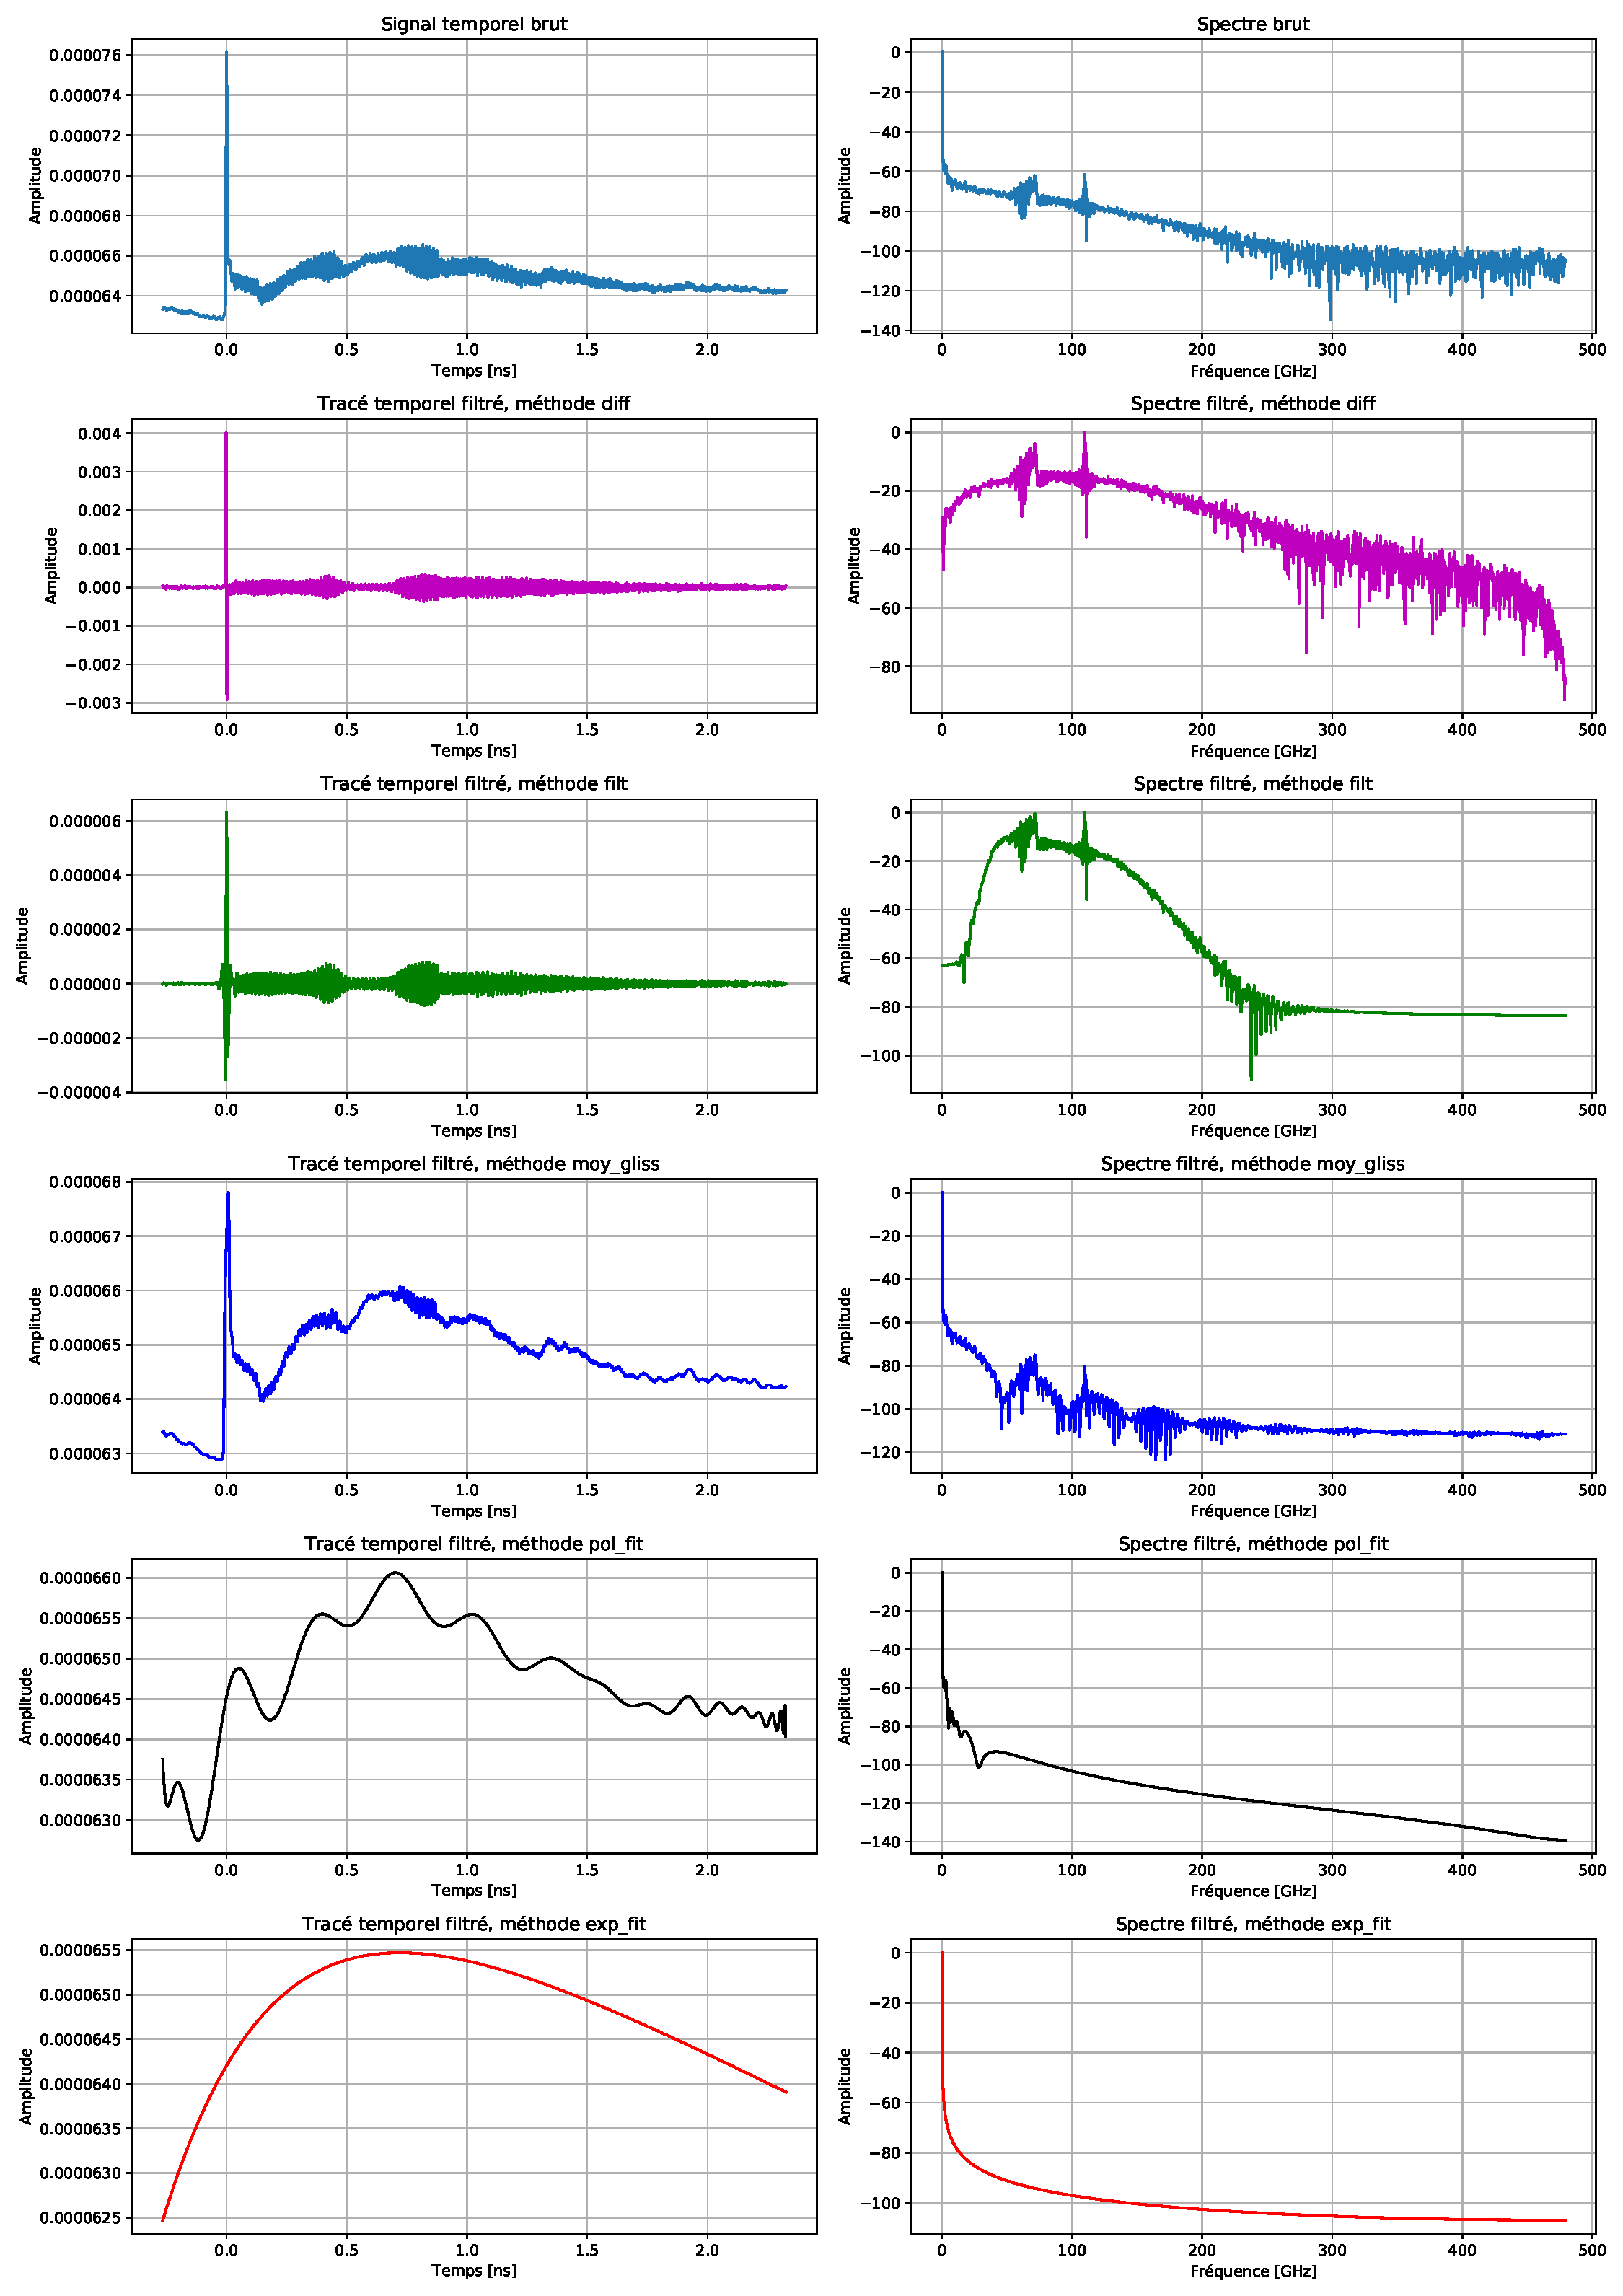
\includepdf[pagecommand={\subsection{Comparaison des différentes méthodes de filtrages pour le projet 4}}, scale=.8]{Figures/tds_methfilt.pdf}

%\subsection{Représentation de la trajectoire des rayons dans les différents systèmes optiques}
\end{document}

